%-------------------------------------------------------------------------------
%                            BAB IV
%               		HASIL DAN PEMBAHASAN
%-------------------------------------------------------------------------------
\fancyhf{} 
\fancyfoot[C]{\thepage}
\chapter{HASIL DAN PEMBAHASAN}
	\section{\uppercase{ANALISIS KEBUTUHAN}}
	
	Hasil dari analisis kebutuhan yang telah dilakukan adalah mendapatkan kelompok pengguna yang akan terlibat dalam penelitian dan \textit{use case diagram} untuk masing-masing pengguna. Berikut hasil analisis kebutuhan dari sistem yang dibangun.
	
	\subsection{Kelompok Pengguna}
	Kelompok pengguna dari aplikasi ini telah dapat diidentifikasikan pada tahap analisis kebutuhan pada sistem. terdapat 2 kelompok pengguna yang menggunakan aplikasi ini:
		 \begin{enumerate}[1.]
		 	\item Peneliti
		 		\newline Pengguna yang menggunakan Aplikasi Mapping berbasis Android untuk melakukan pemetaan kekuatan sinyal atau nilai RSSI dari Beacon. 
		 	\item Dosen
		 		\newline Pengguna yang menggunakan Aplikasi Kehadiran Dosen berbasis Android untuk melakukan pencatatan kehadiran sebagai pengajar suatu mata kuliah.
		 	\item Mahasiswa
		 		\newline Pengguna yang menggunakan Aplikasi Kehadiran berbasis Android untuk melakukan pencatatan kehadiran sebagai peserta belajar suatu mata kuliah.
		 	\item Admin
		 		\newline Pengguna yang menggunakan Aplikasi Rekap Kehadiran Dosen dan Mahasiswa berbasis web untuk memantau dan merekap kehadiran dosen dan mahasiswa pada suatu mata kuliah.
		 	\end{enumerate}
	
	\subsection{Use Case Diagram}
	\textit{Use case} merupakan pemodelan untuk mendeskripsikan sebuah interaksi antara satu atau lebih aktor dengan sistem yang dibuat. Secara kasar, \textit{use case} digunakan untuk mengetahui fungsi apa saja yang ada di dalam sebuah sistem dan siapa saja yang berhak menggunakan fungsi-fungsi itu \citep{Rosa2015}. \textit{Use Case Diagram} dari sistem yang telah dibangun dapat dilihat pada Gambar \ref{usecasemapping}, Gambar \ref{usecasedosen}, Gambar \ref{usecasemahasiswa} dan Gambar \ref{usecaseadmin}.
	
	\begin{figure}[H]
		\center
		\shadowbox
		{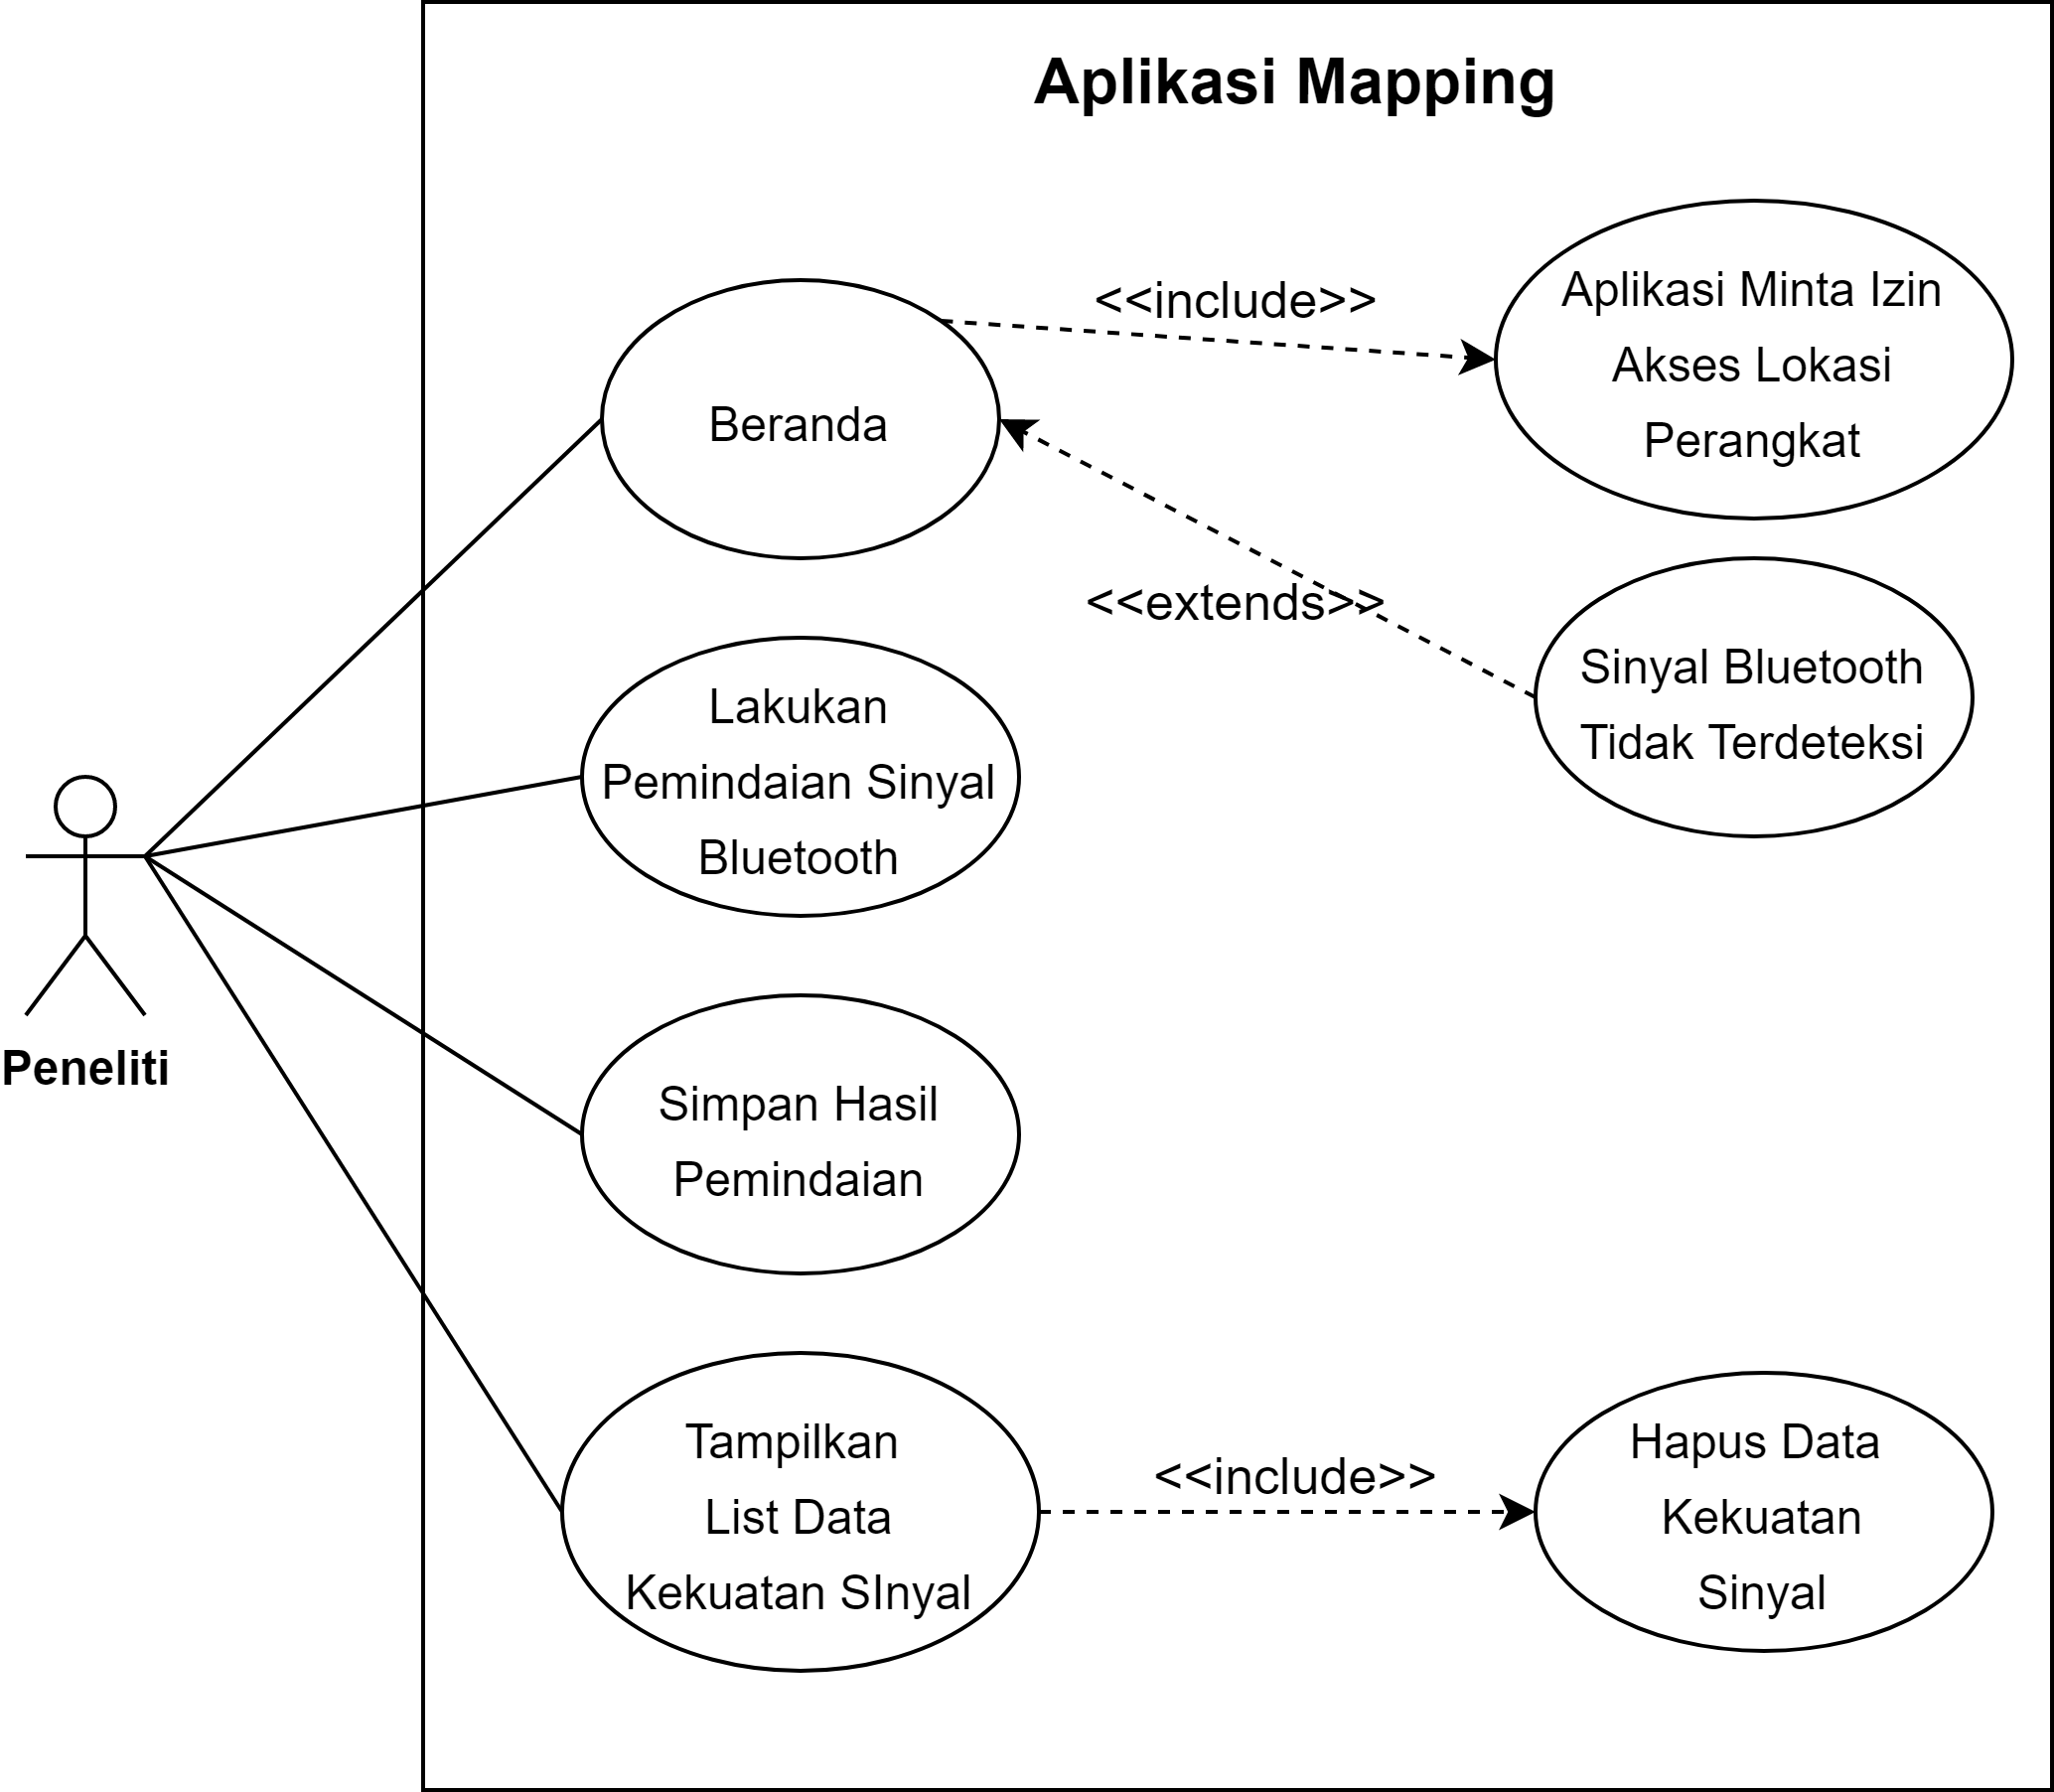
\includegraphics [width=7.5cm, height=7cm]{gambar/model/use-case-mapping}}
		\caption{\textit{Use Case Diagram} Aplikasi Mapping.}
		\label{usecasemapping}
	\end{figure}
	
\par Gambar \ref{usecasemapping} diatas menjelaskan aktivitas yang dapat dilakukan oleh peneliti saat menggunakan aplikasi. Ketika peneliti membuka aplikasi, muncul halaman beranda. Selanjutnya, peneliti diminta untuk mengizinkan aplikasi mengakses lokasi pada perangkat. Kemudian, peneliti dapat melakukan pemindaian kekuatan sinyal setelah menghidupkan Bluetooth pada perangkat. Setelah itu, hasil dari pemindaian kekuatan sinyal tersebut disimpan, lalu dapat ditampilkan pada sebuah halaman. Pengguna juga dapat menghapus data-data kekuatan sinyal sesuai keinginan.
\fancyhf{} 
\fancyfoot[R]{\thepage}

\begin{figure}[H] 
		\center
		\shadowbox
		{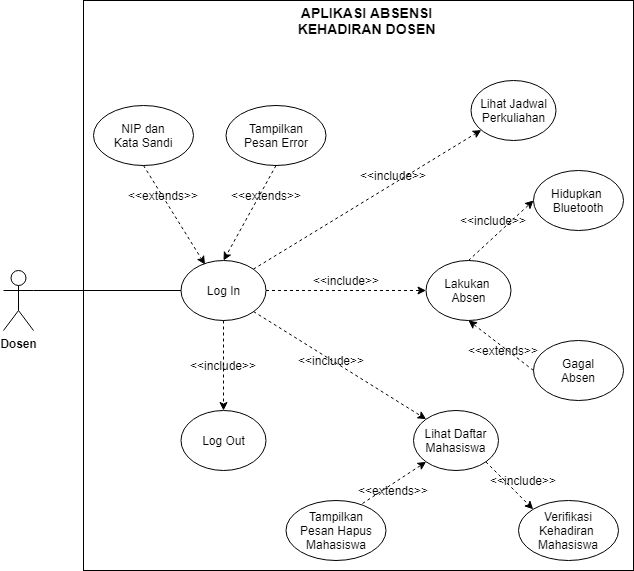
\includegraphics [width=10cm, height=9cm]{gambar/model/use-case-dosen}}
		\caption{\textit{Use Case Diagram} Aplikasi Kehadiran Dosen.}
		\label{usecasedosen}
	\end{figure}

\par Gambar \ref{usecasedosen} menjelaskan aktivitas yang dapat dilakukan oleh dosen saat menggunakan aplikasi. Aktivitas pertama yang dilakukan adalah melakukan \textit{log in} ke aplikasi dengan memasukkan Nomor Induk Pegawai (NIP) dan kata sandi. Setelah melakukan \textit{log in}, dosen dapat menikmati fitur-fitur yang tersedia seperti melihat jadwal perkuliahan, memulai proses kehadiran dengan syarat keadaan Bluetooth pada perangkat dalam keadaan hidup dan melihat daftar mahasiswa yang mengambil suatu mata kuliah. Aktivitas yang terakhir adalah \textit{log out}, yaitu aktivitas yang berfungsi untuk keluar dari aplikasi. Apabila dosen telah melakukan \textit{log out}, maka dosen harus melakukan \textit{log in} kembali ke aplikasi.
	
	\begin{figure}[H] 
		\center
		\shadowbox
		{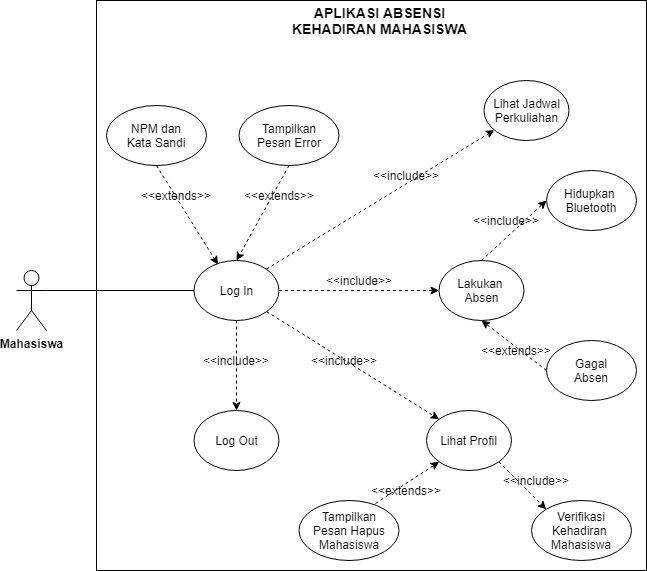
\includegraphics [width=10cm, height=9.5cm]{gambar/model/use-case-mahasiswa}}
		\caption{\textit{Use Case Diagram} Aplikasi Kehadiran Mahasiswa.}
		\label{usecasemahasiswa}
	\end{figure}
	
\par Gambar \ref{usecasemahasiswa} diatas menjelaskan aktivitas yang dapat dilakukan oleh mahasiswa saat menggunakan aplikasi. Aktivitas pertama yang dilakukan adalah melakukan \textit{log in} ke aplikasi dengan memasukkan Nomor Pokok Mahasiswa (NPM) dan kata sandi. Setelah melakukan \textit{log in}, mahasiswa dapat menikmati fitur-fitur yang tersedia seperti melihat jadwal perkuliahan, memulai proses kehadiran dengan syarat keadaan Bluetooth pada perangkat dalam keadaan hidup dan melihat profil data diri. Aktivitas yang terakhir adalah \textit{log out}, yaitu aktivitas yang berfungsi untuk keluar dari aplikasi. Apabila mahasiswa telah melakukan \textit{log out}, maka mahasiswa harus melakukan \textit{log in} kembali ke aplikasi.

	\begin{figure}[H] 
		\center
		\shadowbox
		{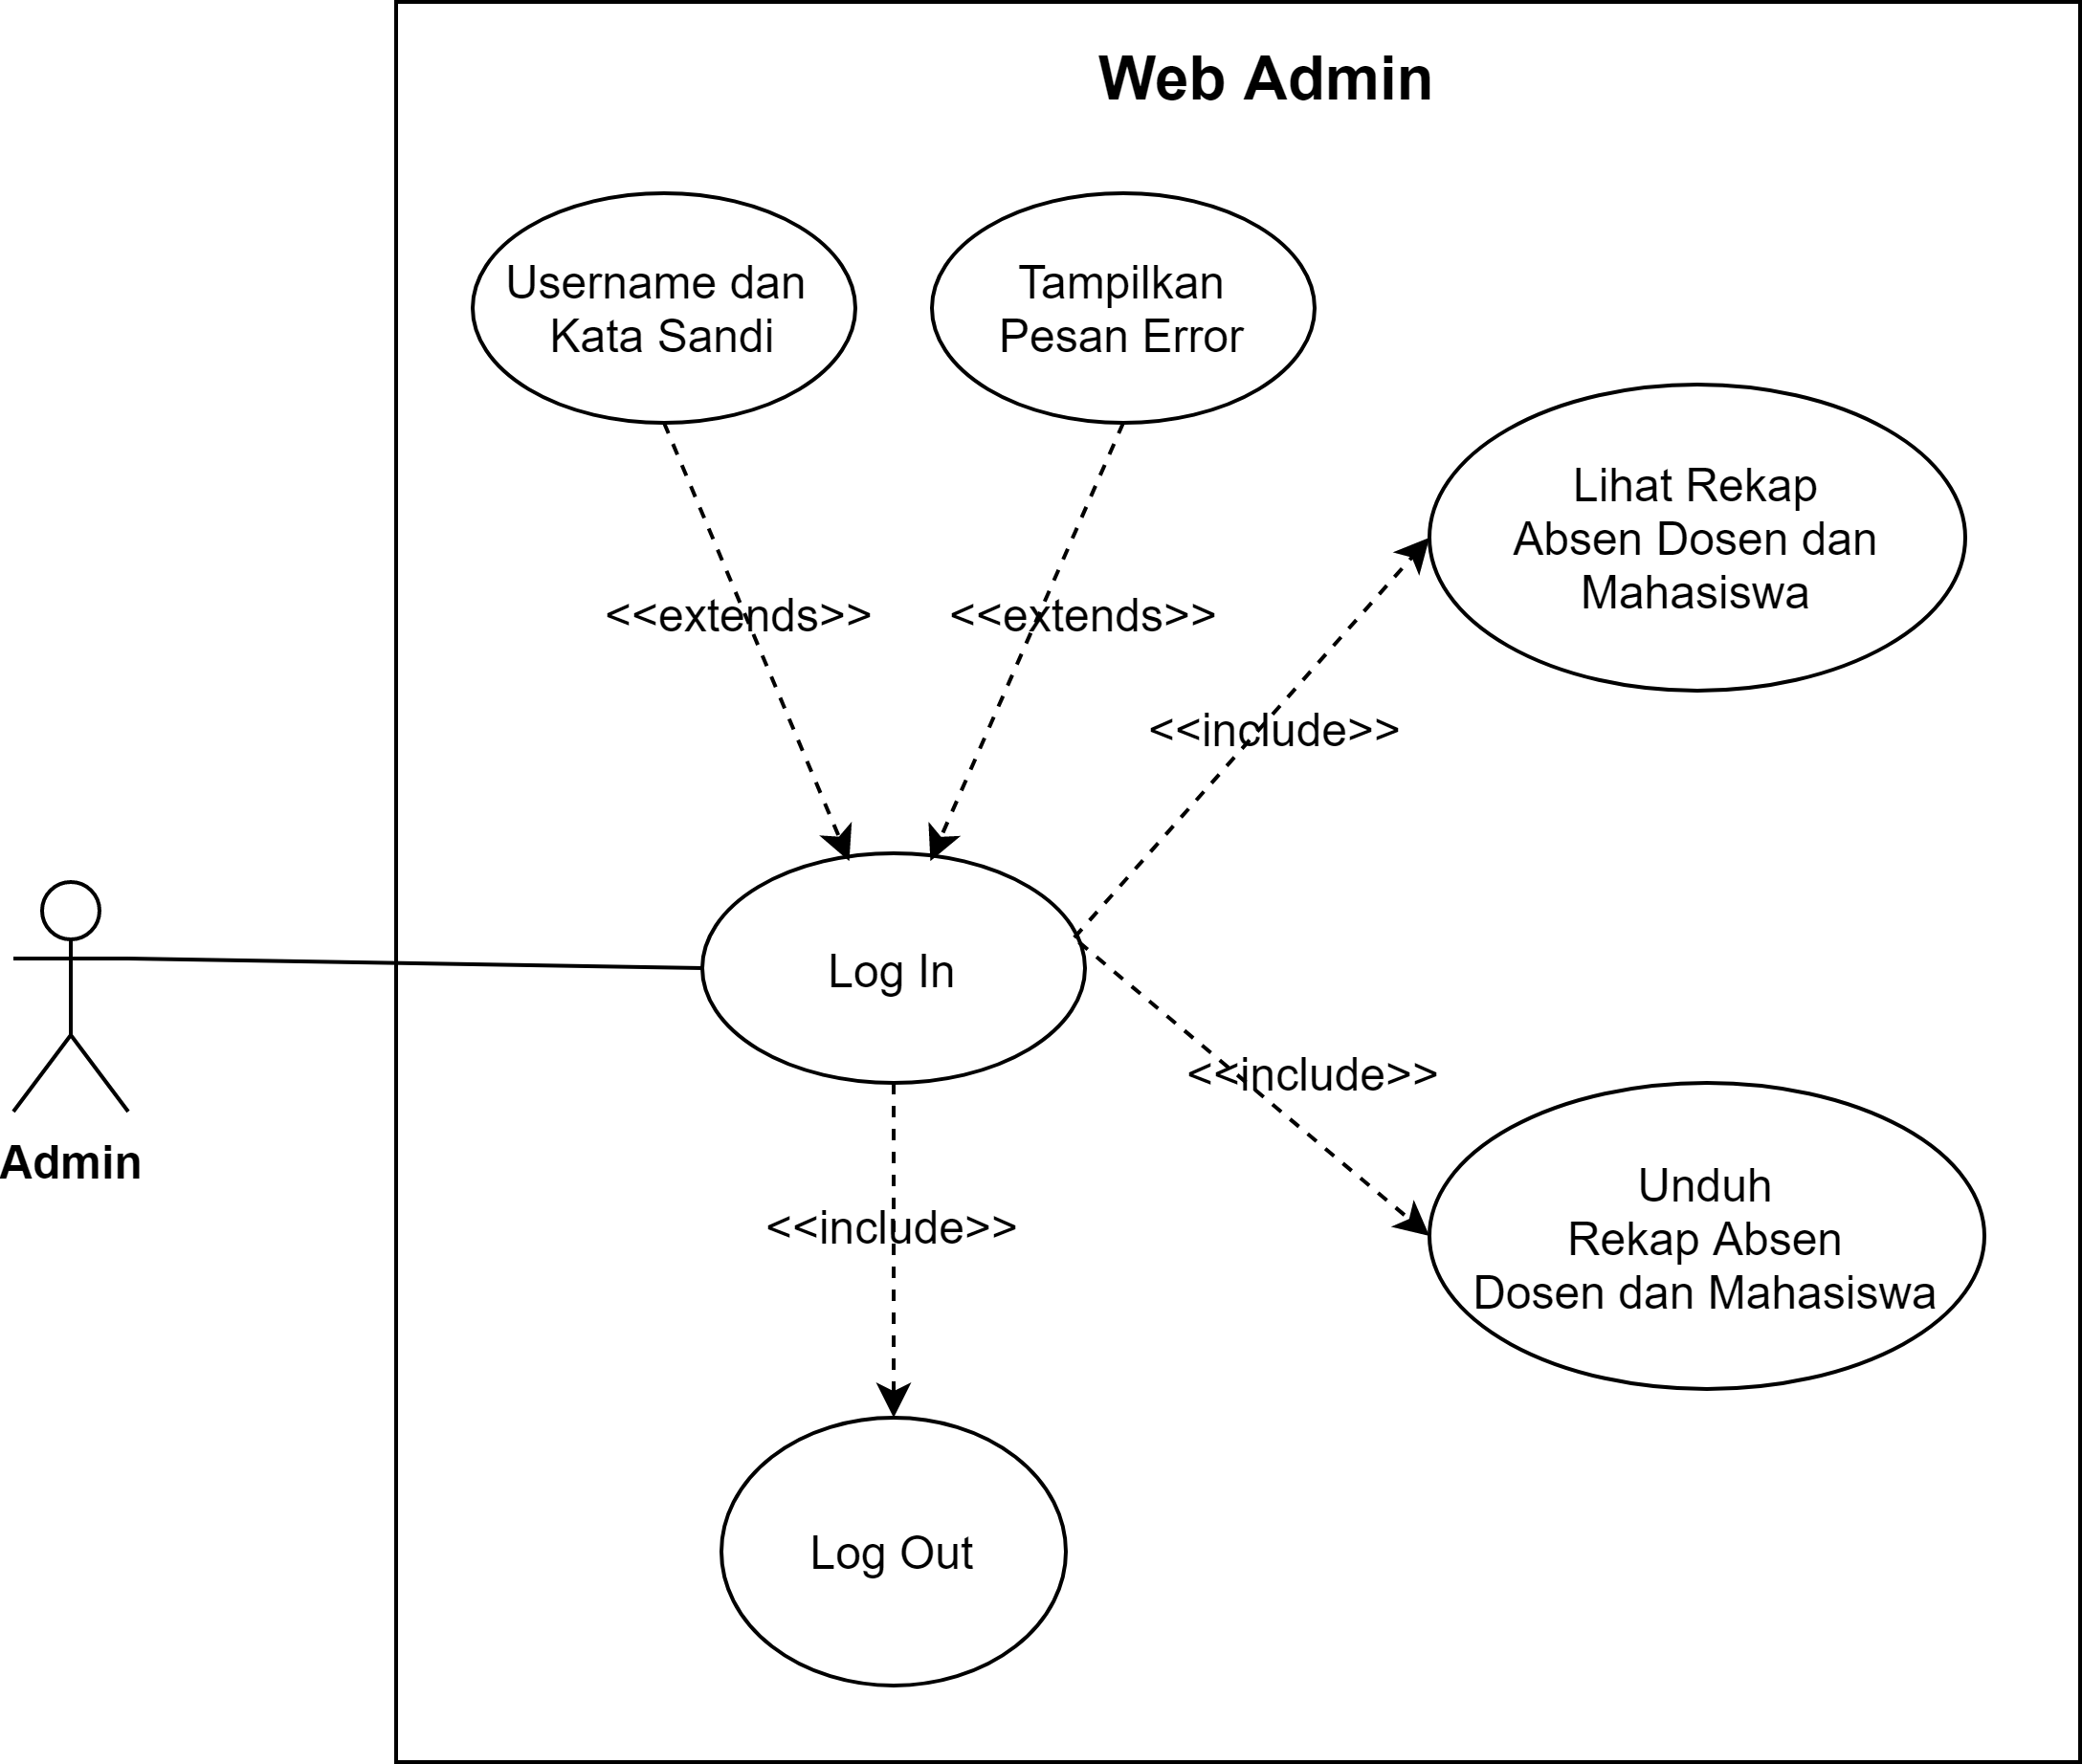
\includegraphics [width=9cm, height=8cm]{gambar/model/use-case-admin}}
		\caption{\textit{Use Case Diagram} Aplikasi Rekap Kehadiran Dosen dan Mahasiswa (Web-Based).}
		\label{usecaseadmin}
	\end{figure}
	
\par Gambar \ref{usecaseadmin} diatas menjelaskan aktivitas yang dapat dilakukan oleh admin saat menggunakan aplikasi. Aktivitas pertama yang dilakukan adalah melakukan \textit{log in} ke aplikasi dengan memasukkan \textit{username} dan kata sandi. Setelah melakukan \textit{log in}, admin dapat melihat daftar kehadiran dosen dan mahasiswa pada mata kuliah tertentu. Selain itu, admin juga dapat mengunduh data-data kehadiran tersebut.
	


	\section{\uppercase{PERANCANGAN DAN PEMBUATAN SISTEM}}
	
	\subsection{Perancangan Sistem}
	\par Perancangan sistem merupakan tahapan proses desain dari sistem perangkat lunak yang dibuat. Proses ini terdiri dari dua tahap yaitu perancangan konfigurasi eksekusi sistem dalam bentuk \textit{deployment diagram} dan perancangan tampilan antar muka (\textit{interface}).
	
   	%Tahap pertama adalah merancang \textit{class diagram} yang bertujuan untuk menggambarkan struktur sistem dari segi pendefinisian dari kelas-kelas yang dibuat untuk membangun sistem. Kelas-kelas yang ada pada struktur sistem harus dapat melakukan fungsi-fungsi sesuai dengan kebutuhan sistem. %Berikut rancangan \textit{class diagram} dari sistem yang telah dibangun dapat dilihat pada Gambar:
   			%\begin{enumerate}
     			%\item \textit{Class Diagram} Aplikasi Mapping
					%\vspace{-0.2cm}
					%\begin{figure}[H]
						%\center
						%\includegraphics [width = 14cm]{gambar/model/class-diagram}
						%\caption{Diagram Kelas Model Basis Data }
					%\label{class}
					%\end{figure}
									
     			%\item \textit{Class Diagram} Aplikasi Kehadiran Dosen
     			%\item \textit{Class Diagram} Aplikasi Kehadiran Mahasiswa
   			%\end{enumerate}
 	%Tahap kedua adalah merancang \textit{component diagram}, dimana \textit{component diagram} dibuat untuk menunjukkan organisasi dan ketergantungan diantara kumpulan komponen dalam sebuah sistem, serta pemodelan bagaimana sistem beradaptasi dengan sistem lain. Berikut rancangan \textit{component diagram} dari sistem yang telah dibangun dapat dilihat pada Gambar \ref{componentmapping} dan Gambar \ref{componentabsensi}.
 			%\begin{enumerate}
     			%\item \textit{Component Diagram} Aplikasi Mapping
					%\vspace{-0.2cm}
					%\begin{figure}[H]
						%\center
						%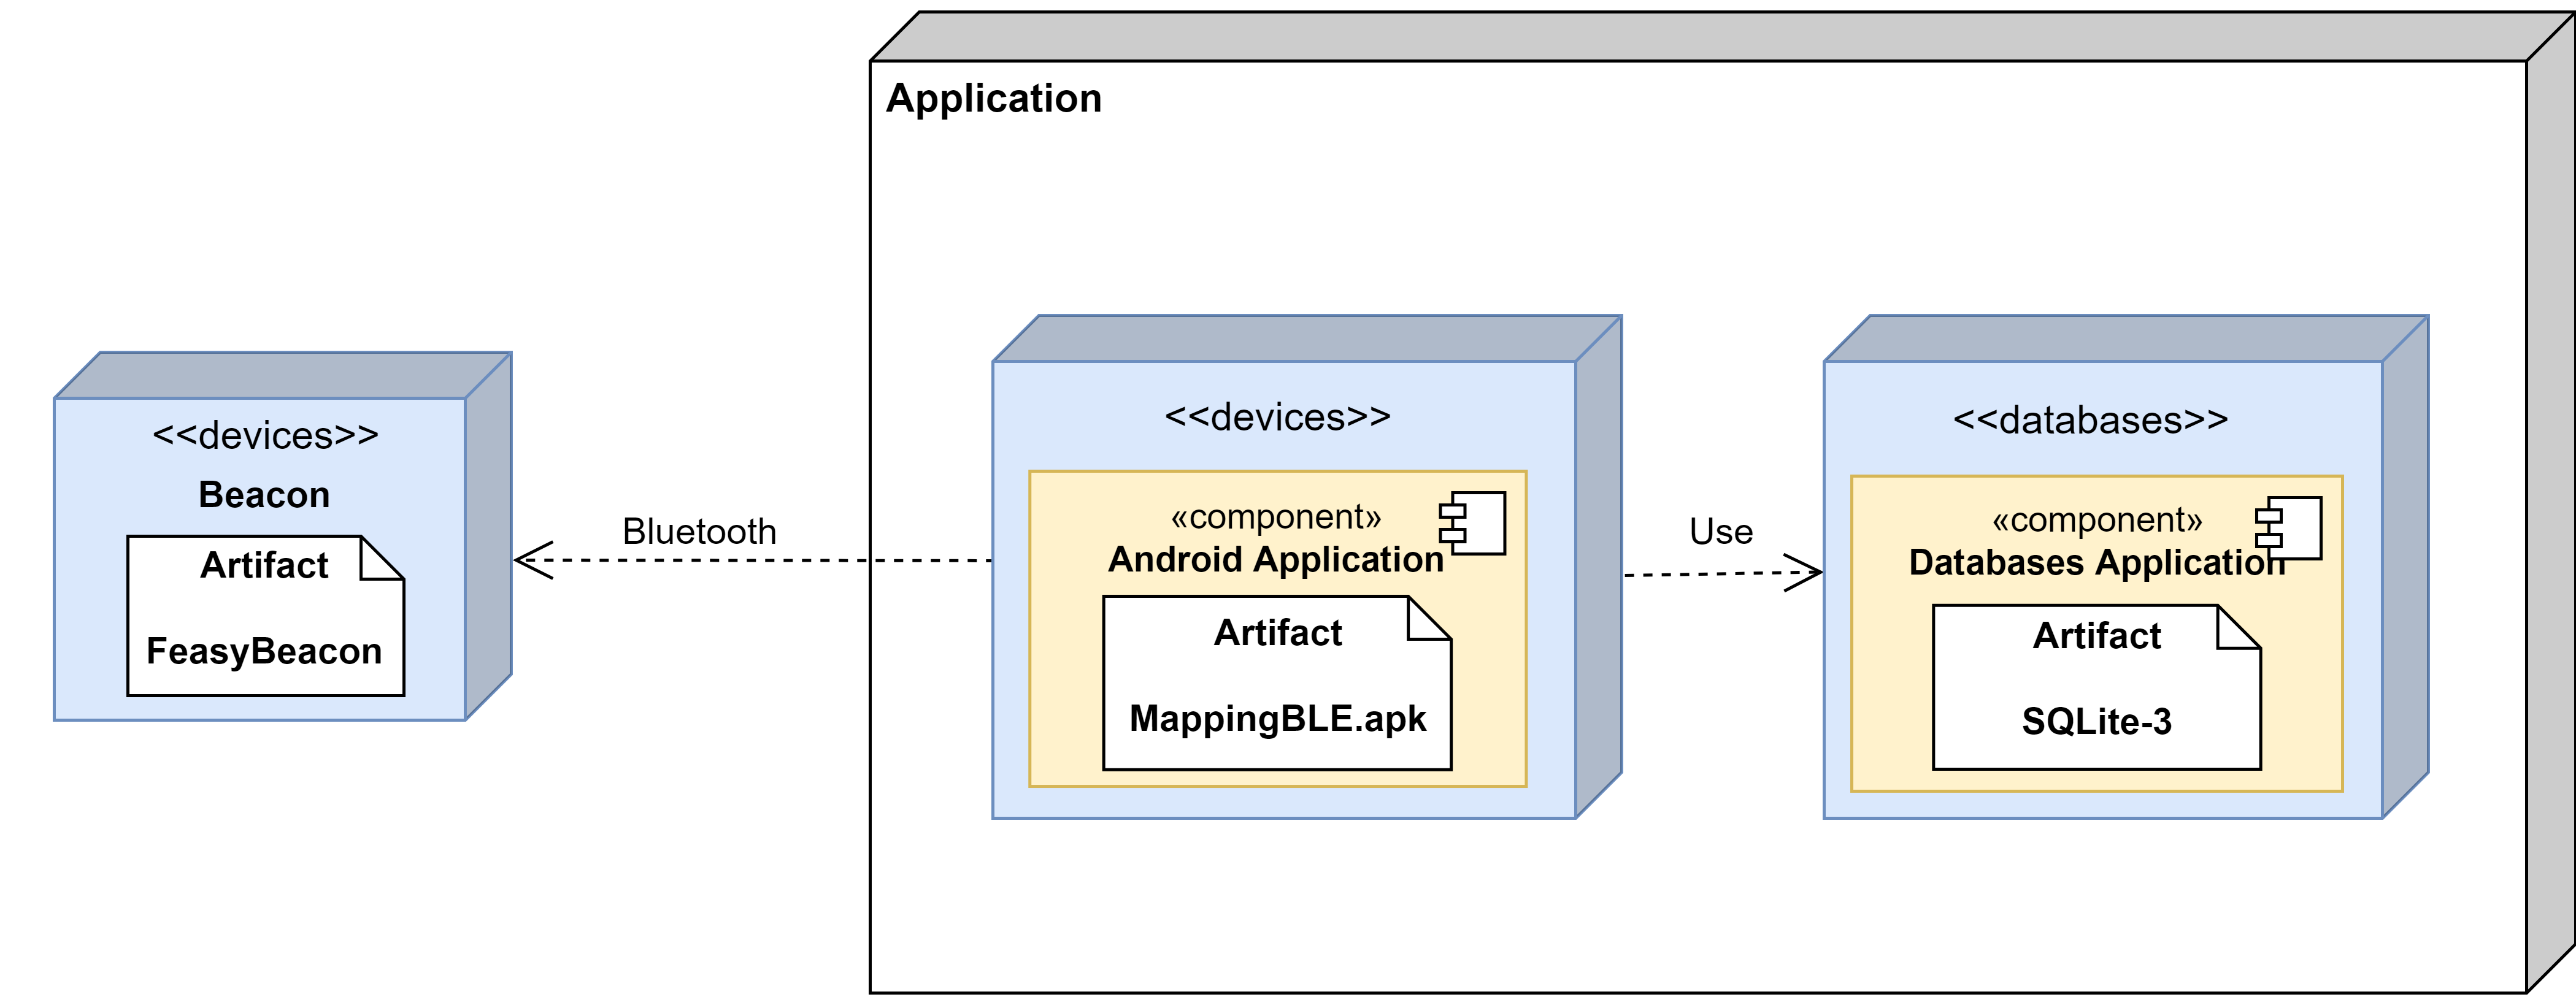
\includegraphics [width = 13cm, height= 5cm]{gambar/model/component-diagram-mapping}
						%\caption{Diagram Component Aplikasi Mapping}
					%\label{componentmapping}
					%\end{figure}
									
     			%\item \textit{Component Diagram} Aplikasi Kehadiran Dosen dan Aplikasi Kehadiran Mahasiswa
     				%\vspace{-0.2cm}
					%\begin{figure}[H]
						%\center
						%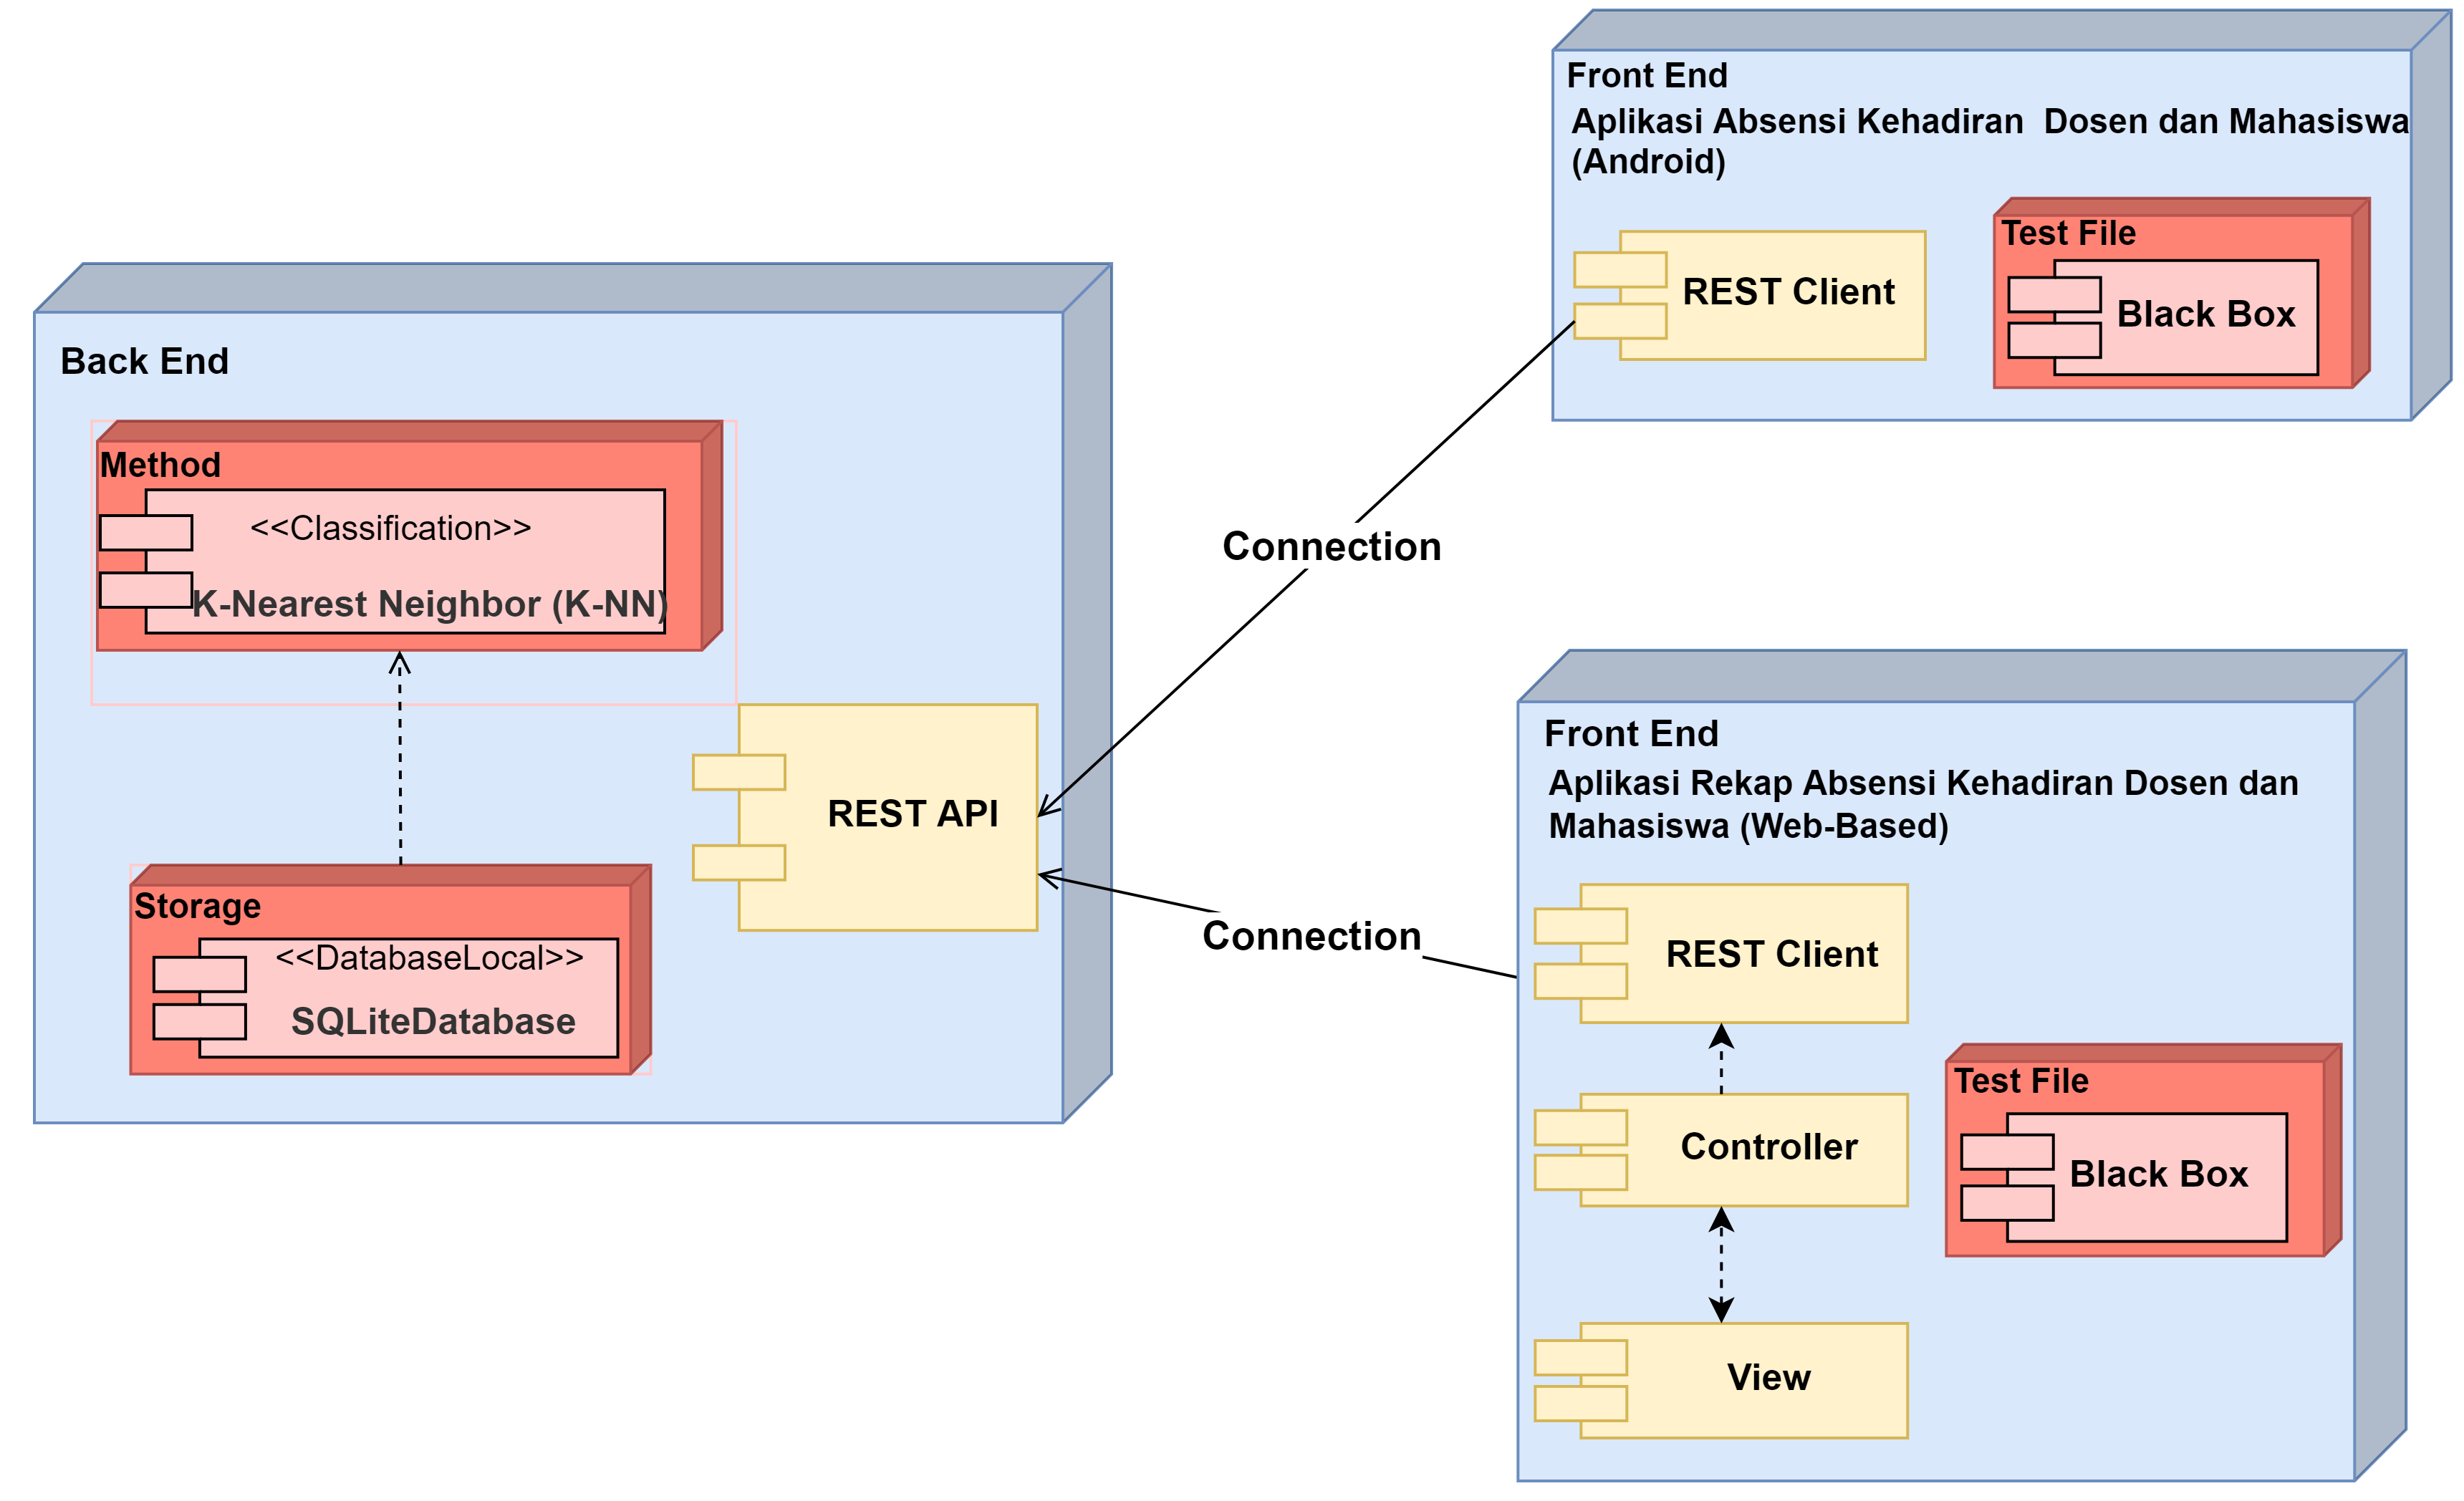
\includegraphics [width = 13.5cm, height= 9cm]{gambar/model/component-diagram-absensi}
						%\caption{Diagram Component Aplikasi Kehadiran Dosen dan Mahasiswa}
					%\label{componentabsensi}
					%\end{figure}
   			%\end{enumerate}
   	Tahap pertama adalah merancang \textit{deployment diagram}, dimana \textit{deployment diagram} adalah diagram yang menjelaskan bagaimana sistem bekerja dan digunakan oleh pengguna. Berikut rancangan \textit{deployment diagram} dari sistem yang telah dibangun dapat dilihat pada Gambar \ref{deployment-diagram}.
   		
 			%\begin{enumerate}
     			%\item \textit{Deployment Diagram} Aplikasi Mapping
					\vspace{-0.2cm}
				 \begin{landscape}
					\begin{figure}[H]
						\center
						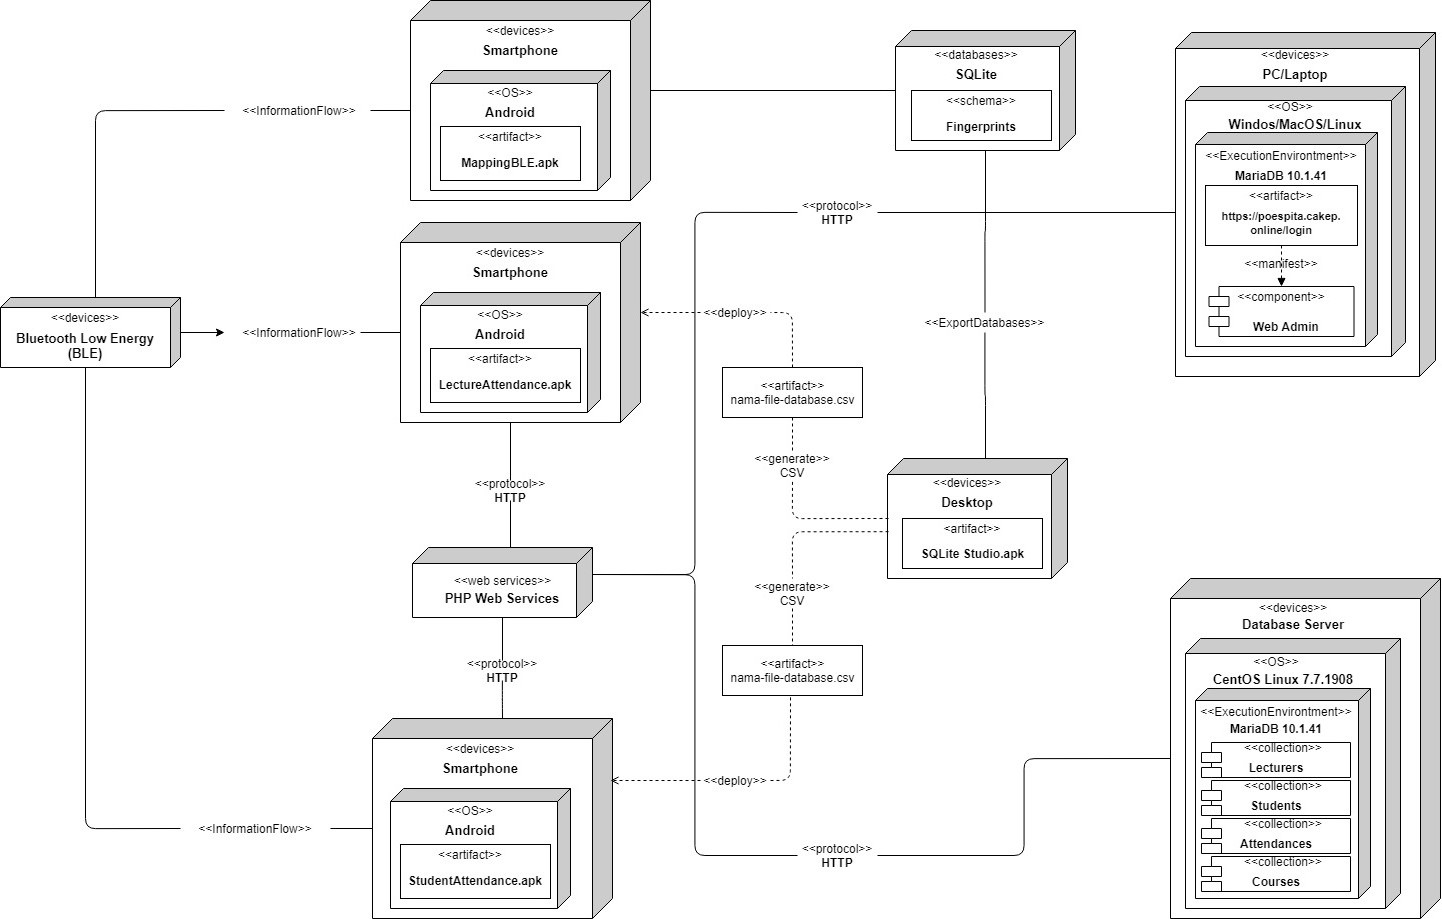
\includegraphics [width = 22.5cm, height=12cm]{gambar/model/deployment-diagram}
						\caption{Diagram \textit{Deployment}}
					\label{deployment-diagram}
					\end{figure}
				  \end{landscape}
									
     			%\item \textit{Deployment Diagram} Aplikasi Kehadiran Dosen dan Aplikasi Kehadiran Mahasiswa
     				%\vspace{-0.2cm}
					%\begin{figure}[H]
						%\center
						%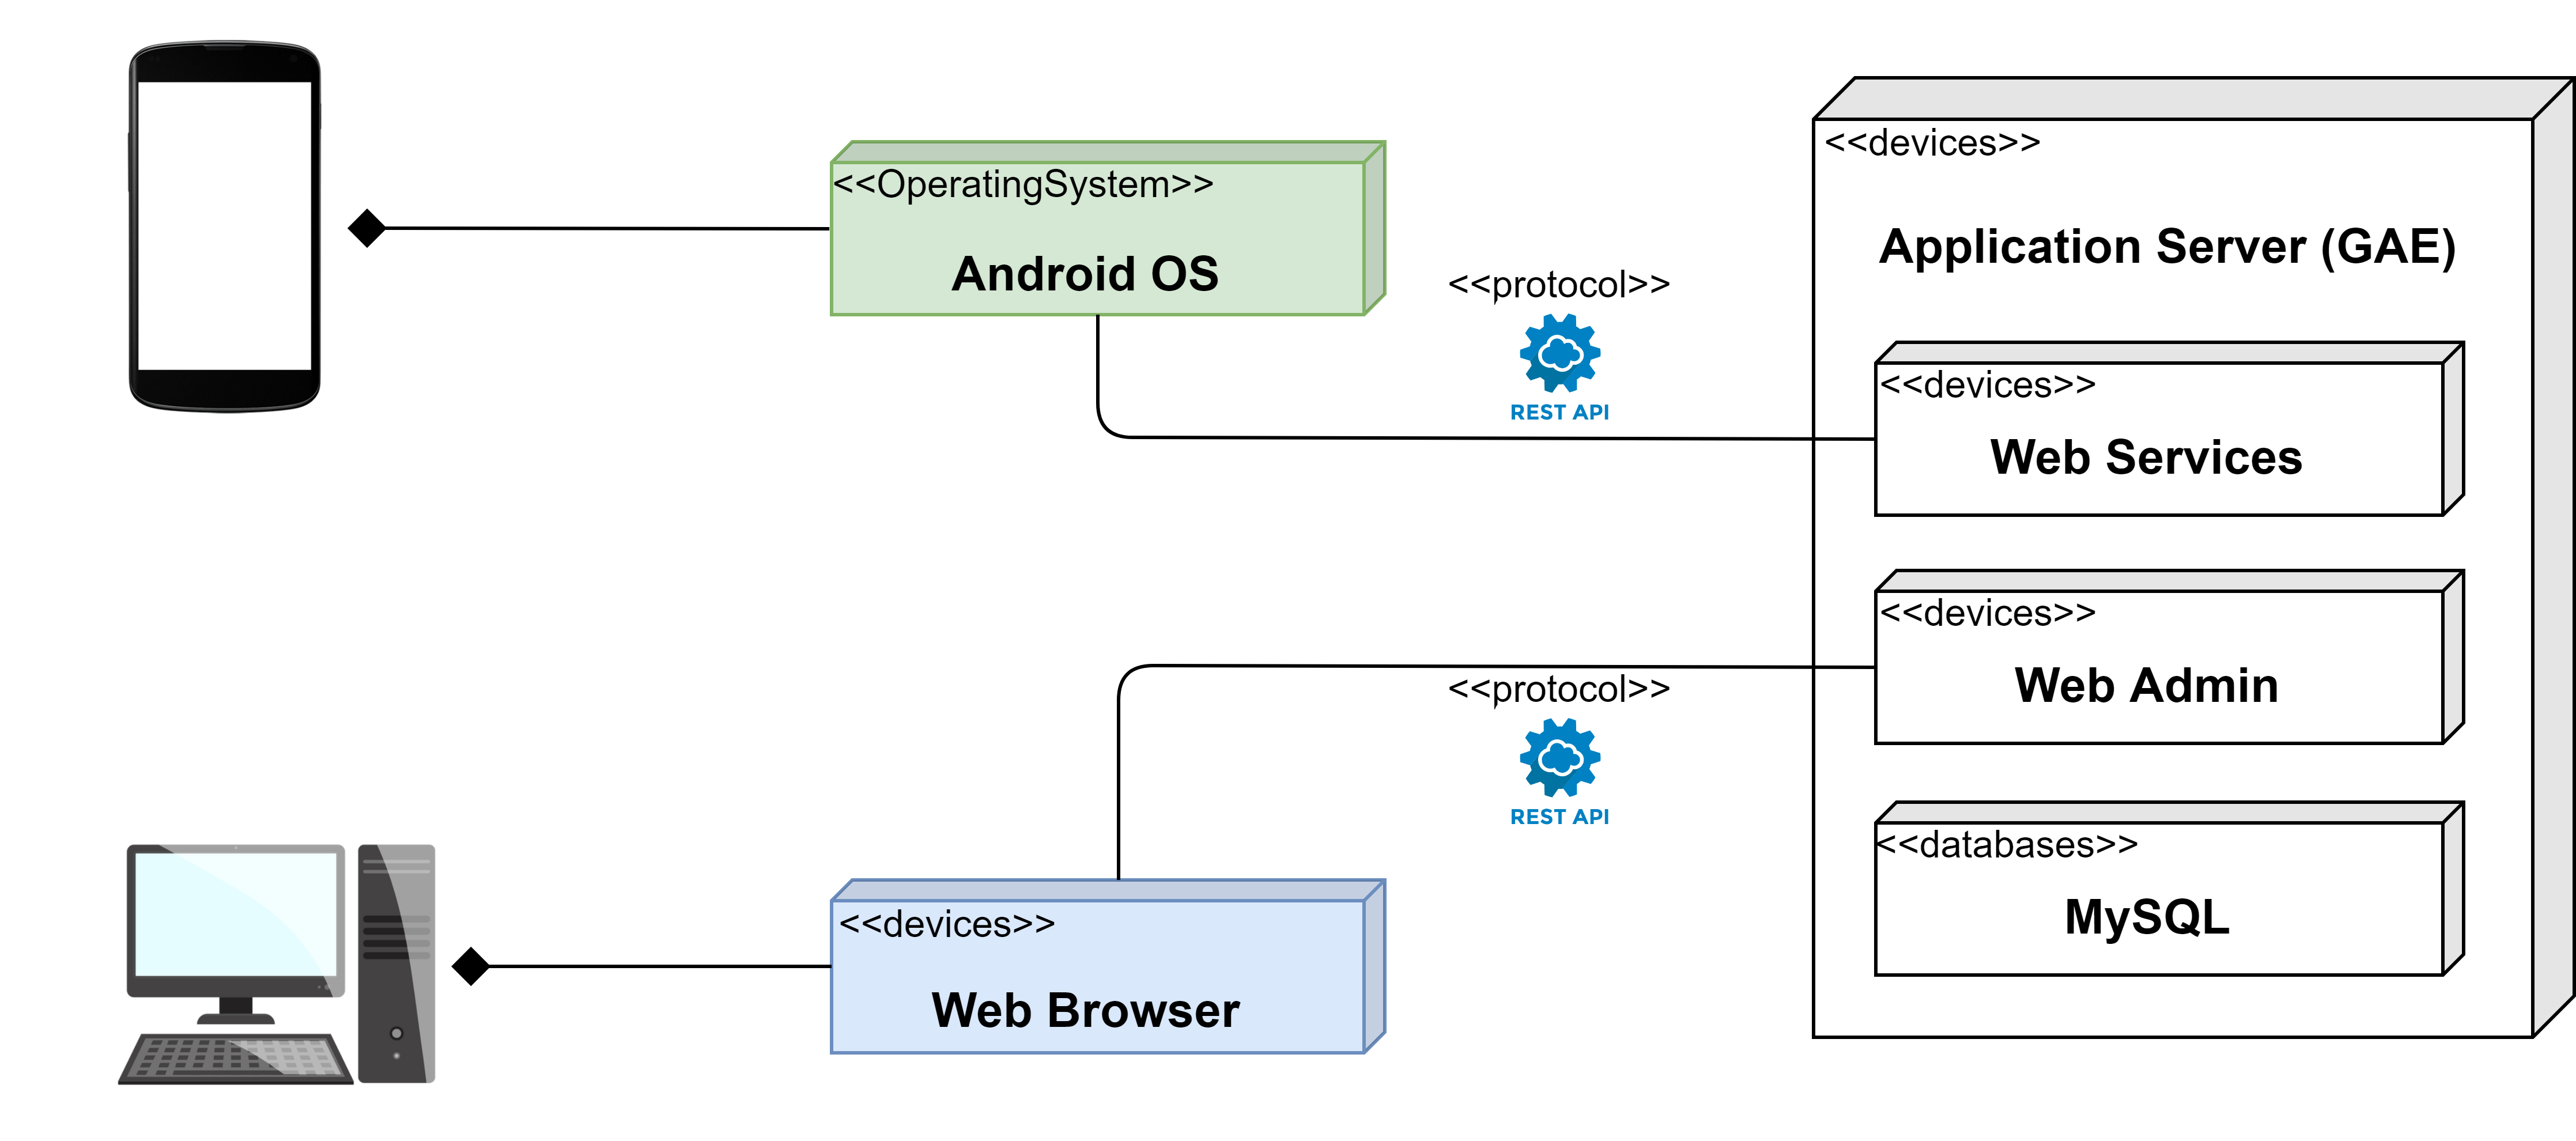
\includegraphics [width = 13.5cm, height= 5.5cm]{gambar/model/deployment-diagram-absensi}
						%\caption{Diagram Deployment Aplikasi Kehadiran Dosen dan Mahasiswa}
					%\label{deploymentabsensi}
					%\end{figure}
   			%\end{enumerate}
 	
	Tahap kedua adalah merancang tampilan antar muka pengguna (\textit{user interface}) sebagai mekanisme komunikasi dengan sistem. Antar muka dari sistem yang telah dibangun adalah sebagai berikut:
		\begin{enumerate}[a.]
		
		\item Antar Muka Aplikasi Mapping
		
		\par Gambar \ref{aplikasimappingbagian1} menampilkan halaman ketika menggunakan aplikasi, kemudian akan muncul notifikasi permintaan izin mengakses lokasi pada perangkat untuk pemindaian kekuatan sinyal Bluetooth. Halaman beranda menampilkan informasi nama ruangan, nama \textit{device} Bluetooth, RSSI dan MAC Address Bluetooth apabila proses pemindaian telah selesai dilakukan serta beberapa tombol untuk memulai proses pemindaian, tombol untuk menyimpan data hasil pemindaian, dan tombol untuk menampilkan data hasil pemindaian.  
				
		\vspace{-0cm}
	\begin{figure} [H]
	\begin{subfigure}{.5\textwidth}
  		\centering
  		% include first image
  		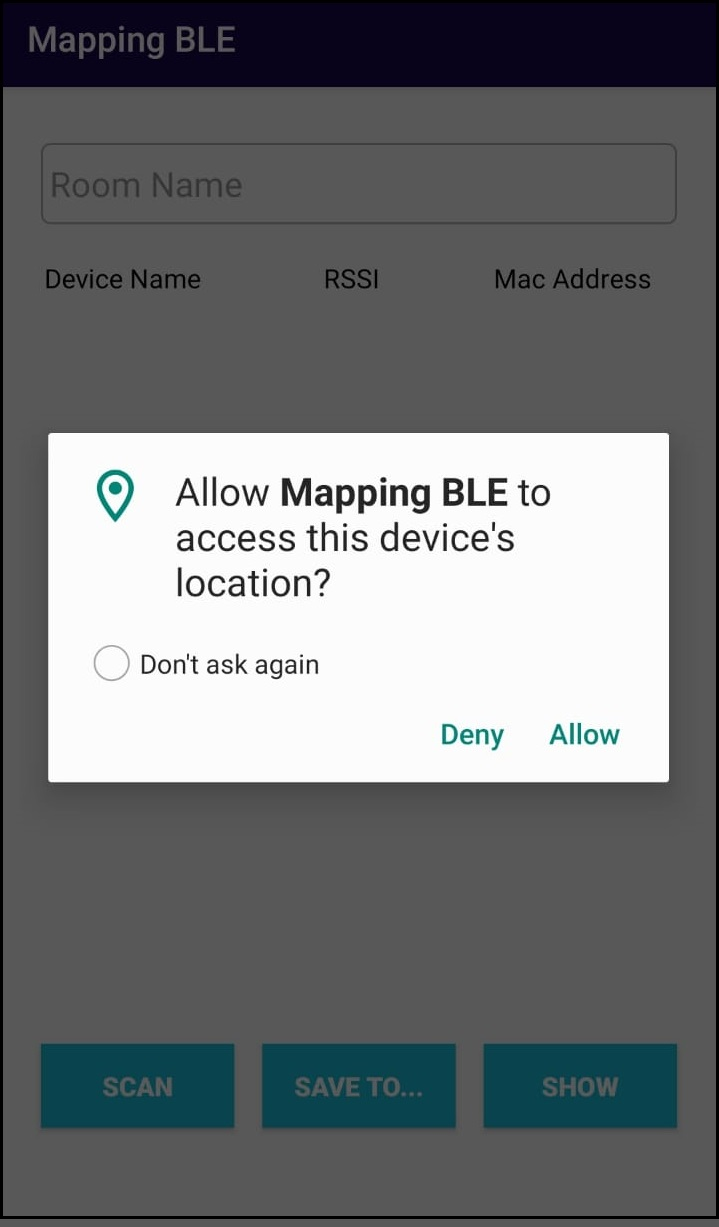
\includegraphics[width=.5\linewidth]{gambar/android/mapping-permission}  
  		\caption{Izin mengakses lokasi}
	\end{subfigure}
	\begin{subfigure}{.5\textwidth}
  		\centering
  		% include second image
		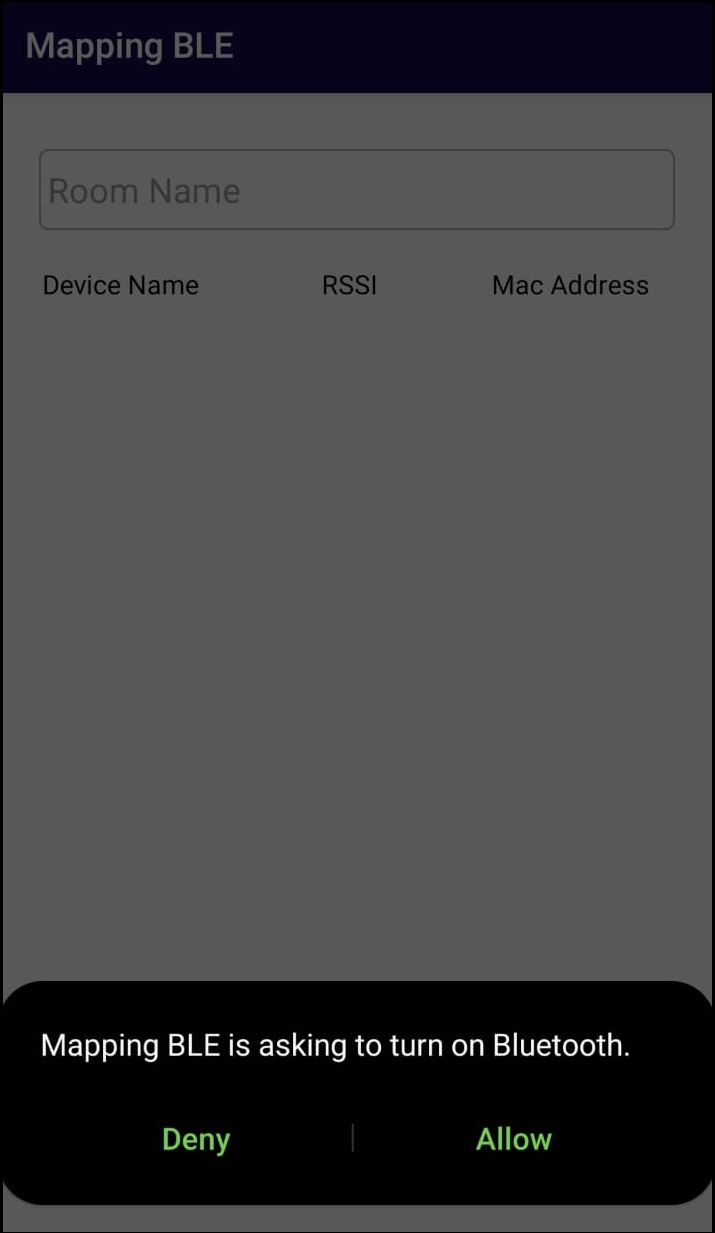
\includegraphics[width=.5\linewidth]{gambar/android/mapping-bluetooth}  
  		\caption{Menghidupkan Bluetooth}
	\end{subfigure}
		\vspace{1cm}
		\newline
	\begin{subfigure}{.5\textwidth}
  		\centering
		 % include third image
	  	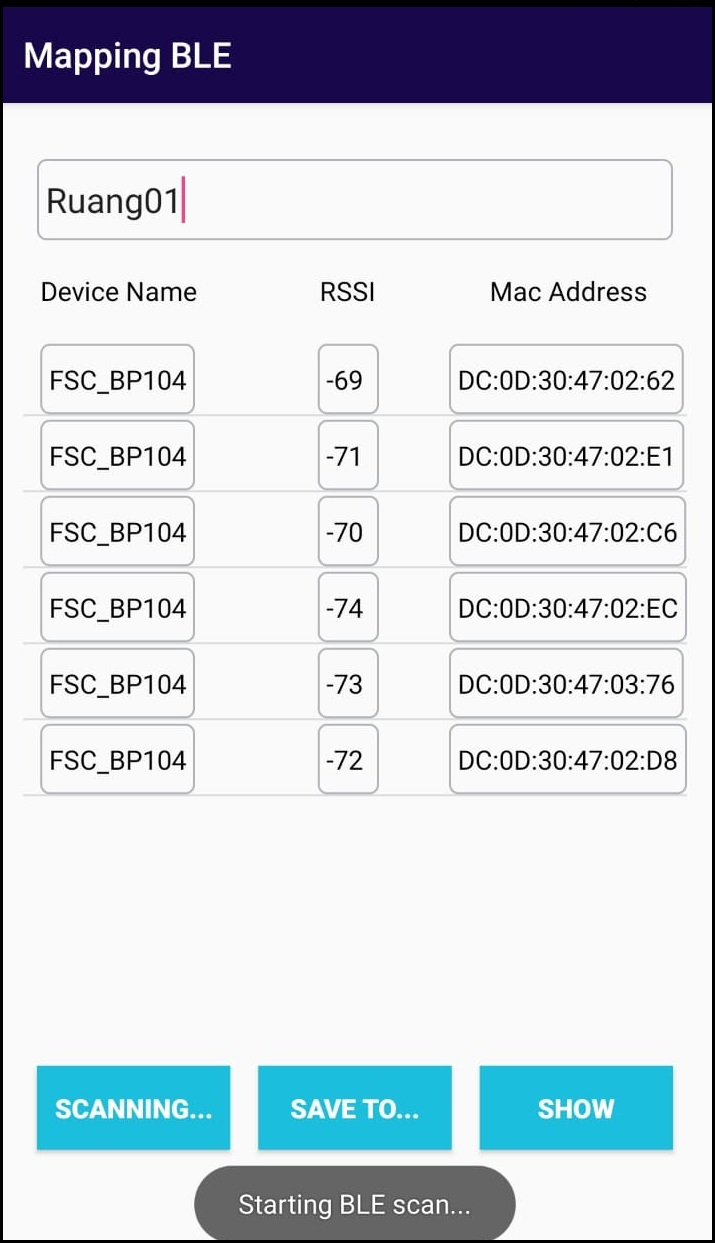
\includegraphics[width=.5\linewidth]{gambar/android/mapping-scanning}  
  		\caption{Proses pemindaian kekuatan sinyal}
	\end{subfigure}
	\begin{subfigure}{.5\textwidth}
  		\centering
  		% include fourth image
  		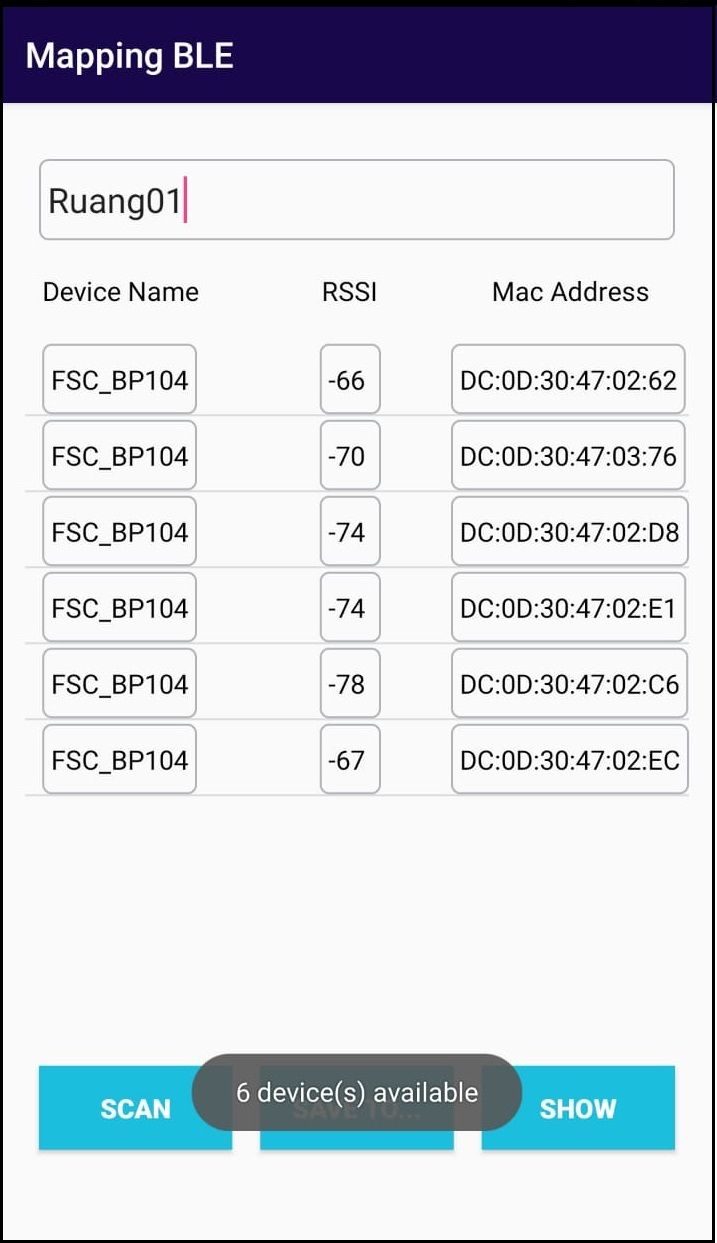
\includegraphics[width=.5\linewidth]{gambar/android/mapping-finish-scan}  
  		\caption{Selesai proses pemindaian}
	\end{subfigure}
		\vspace{0.5cm}
		\caption{Tampilan Halaman Aplikasi Mapping (Bagian 1)}
	\label{aplikasimappingbagian1}
	\end{figure}
	
	\par Apabila pengguna menekan tombol \textbf{save to}, akan muncul \textit{pop up} dimana pengguna dapat memilih tabel penyimpanan data hasil pemindaian, yaitu: tabel \textit{reference point} urut dan tabel \textit{reference point} acak. Jika pengguna menekan tombol \textbf{show data}, akan muncul \textit{pop up} dimana pengguna dapat memilih tabel untuk data yang ingin ditampilkan, kemudian pengguna akan diarahkan ke halaman daftar data hasil pemindaian kekuatan sinyal yang telah disimpan sebelumnya. Jika pengguna ingin menghapus sebuah data, pengguna harus menekan tombol \textit{icon} tong sampah dan lakukan konfirmasi. Fitur-fitur tersebut dapat dilihat pada Gambar \ref{aplikasimappingbagian2}.   
	
	\vspace{-0cm}
	\begin{figure} [H]
	\begin{subfigure}{.5\textwidth}
  		\centering
  		% include first image
  		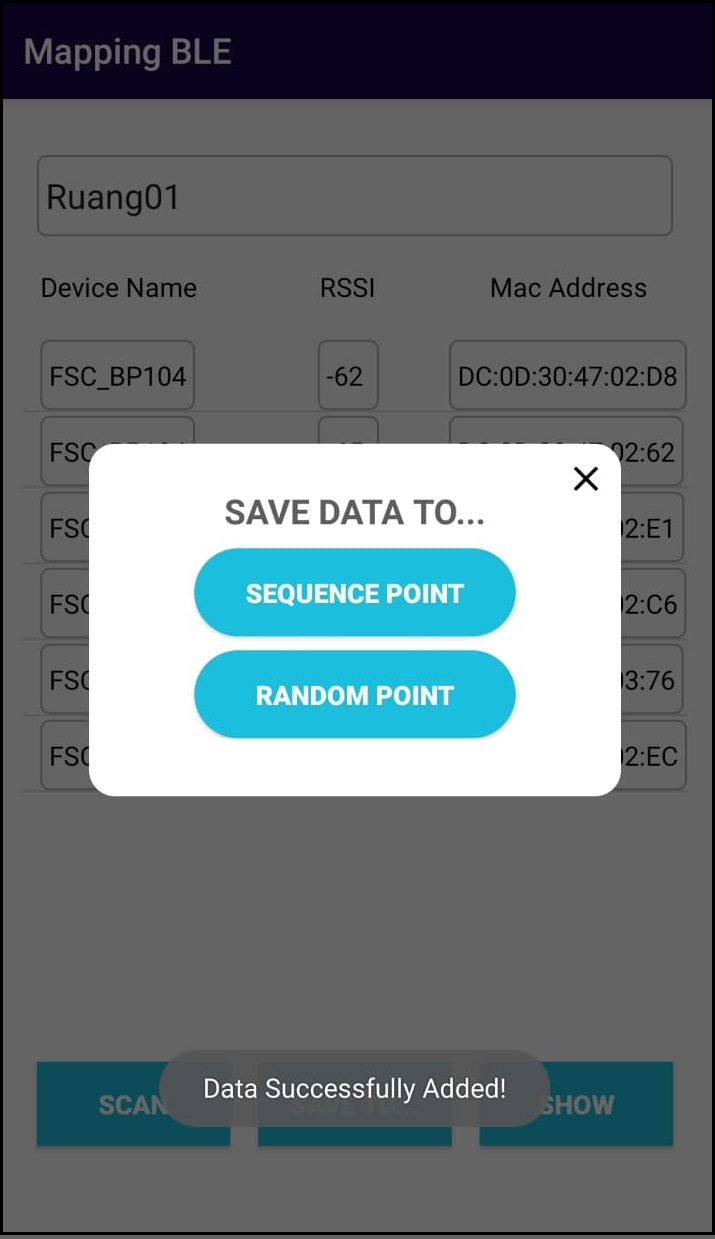
\includegraphics[width=.5\linewidth]{gambar/android/mapping-save-data}  
  		\caption{Simpan hasil pemindaian}
	\end{subfigure}
	\begin{subfigure}{.5\textwidth}
  		\centering
  		% include second image
  		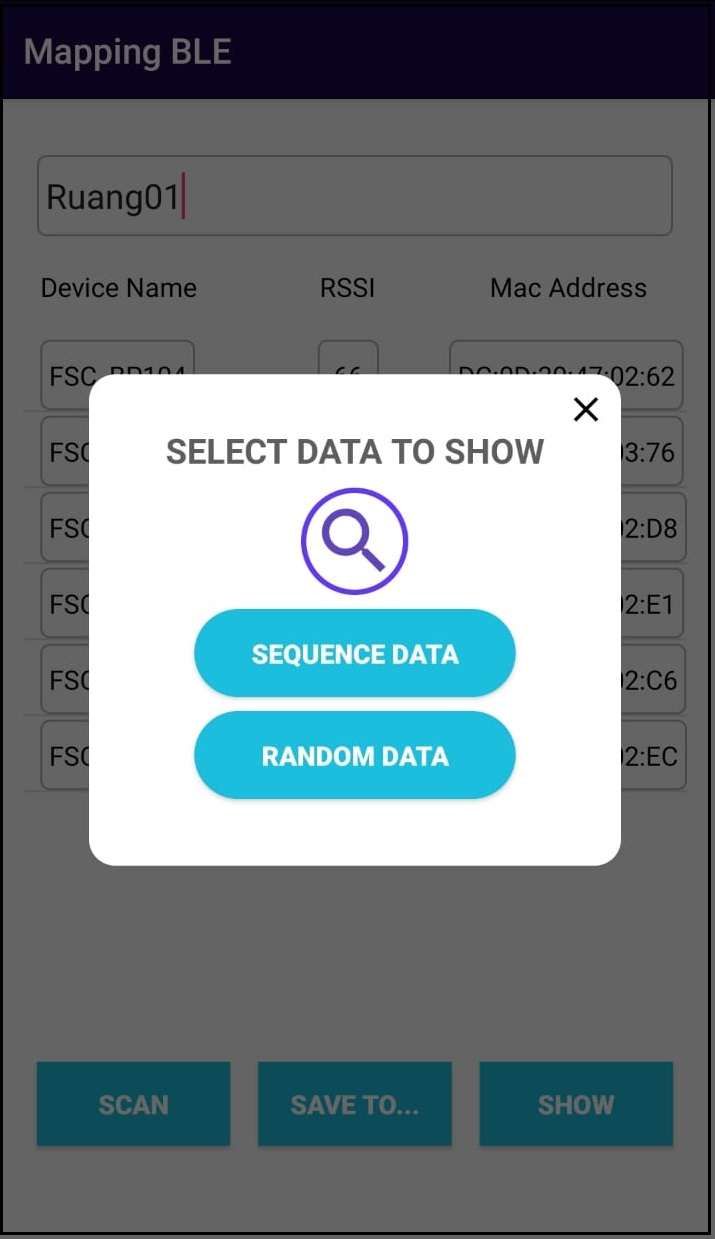
\includegraphics[width=.5\linewidth]{gambar/android/mapping-show-data}  
  		\caption{Pilihan menampilkan data}
	\end{subfigure}
	\vspace{1cm}
	\newline
	\begin{subfigure}{.5\textwidth}
  		\centering
  		% include third image
  		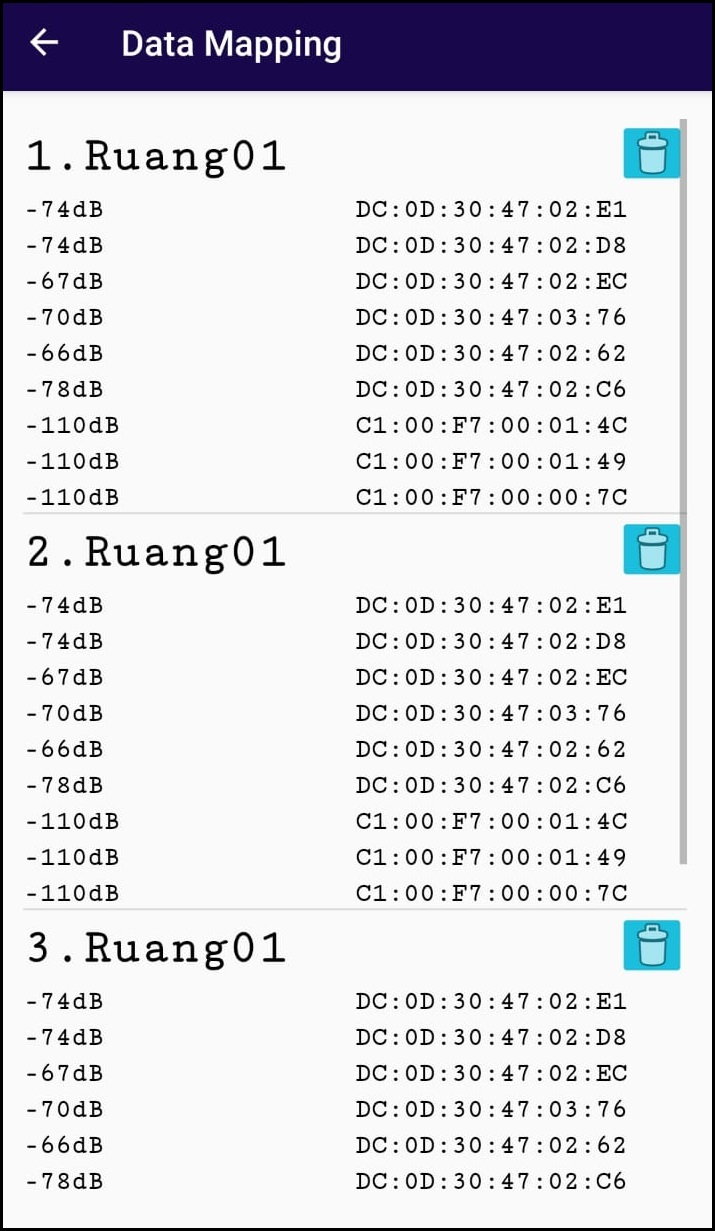
\includegraphics[width=.5\linewidth]{gambar/android/mapping-data-list}  
  		\caption{Menampilkan data yang disimpan}
	\end{subfigure}
	\begin{subfigure}{.5\textwidth}
  		\centering
  		% include fourth image
  		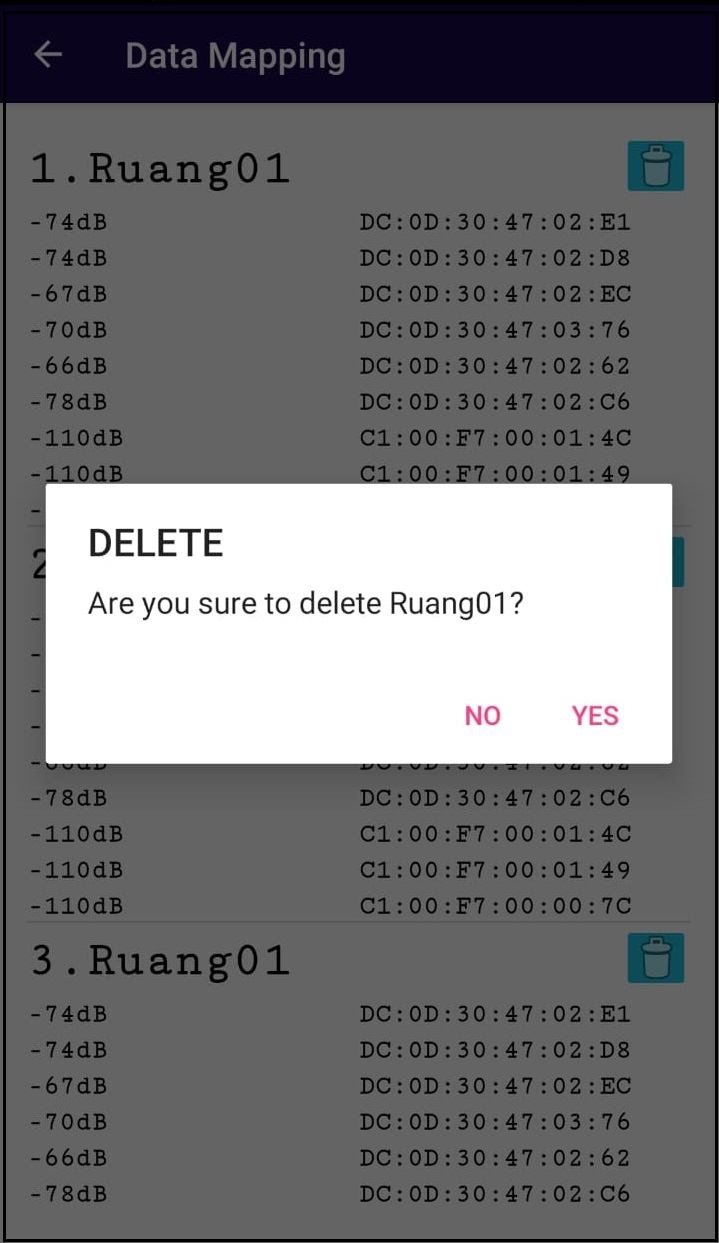
\includegraphics[width=.5\linewidth]{gambar/android/mapping-delete}
  		\caption{Hapus data}
	\end{subfigure}
		\vspace{0.5cm}
		\caption{Tampilan Halaman Aplikasi Mapping (Bagian 2)}
	\label{aplikasimappingbagian2}
	\end{figure}
	%Akhir Gambar Aplikasi Mapping%
	
\vspace{1cm}
		\item Antar Muka Aplikasi Kehadiran Dosen
		
		\par Gambar \ref{aplikasidosenbagian1} memperlihatkan ketika dosen belum melakukan \textit{log in}, aplikasi akan menampilkan \textit{landing page} yang berisi langkah-langkah penggunaan aplikasi, selanjutnya dosen akan diarahkan ke halaman \textit{log in}. Untuk melakukan \textit{log in}, dosen diminta untuk memasukkan Nomor Induk Pegawai (NIP) dan kata sandi yang sesuai dengan Sistem Kepegawaian (SIMPEG) Unsyiah. Setelah itu, dosen akan diarahkan ke halaman beranda apabila telah berhasil melakukan \textit{log in}. Pada halaman beranda, terdapat informasi data diri dosen serta mata kuliah yang diajarkan oleh dosen yang bersangkutan. Jika dosen menekan salah-satu mata kuliah, dosen akan diarahkah ke halaman informasi mata kuliah tersebut.
	\vspace{-0cm}
	\begin{figure} [H]
	\begin{subfigure}{.5\textwidth}
  		\centering
  		% include first image
  		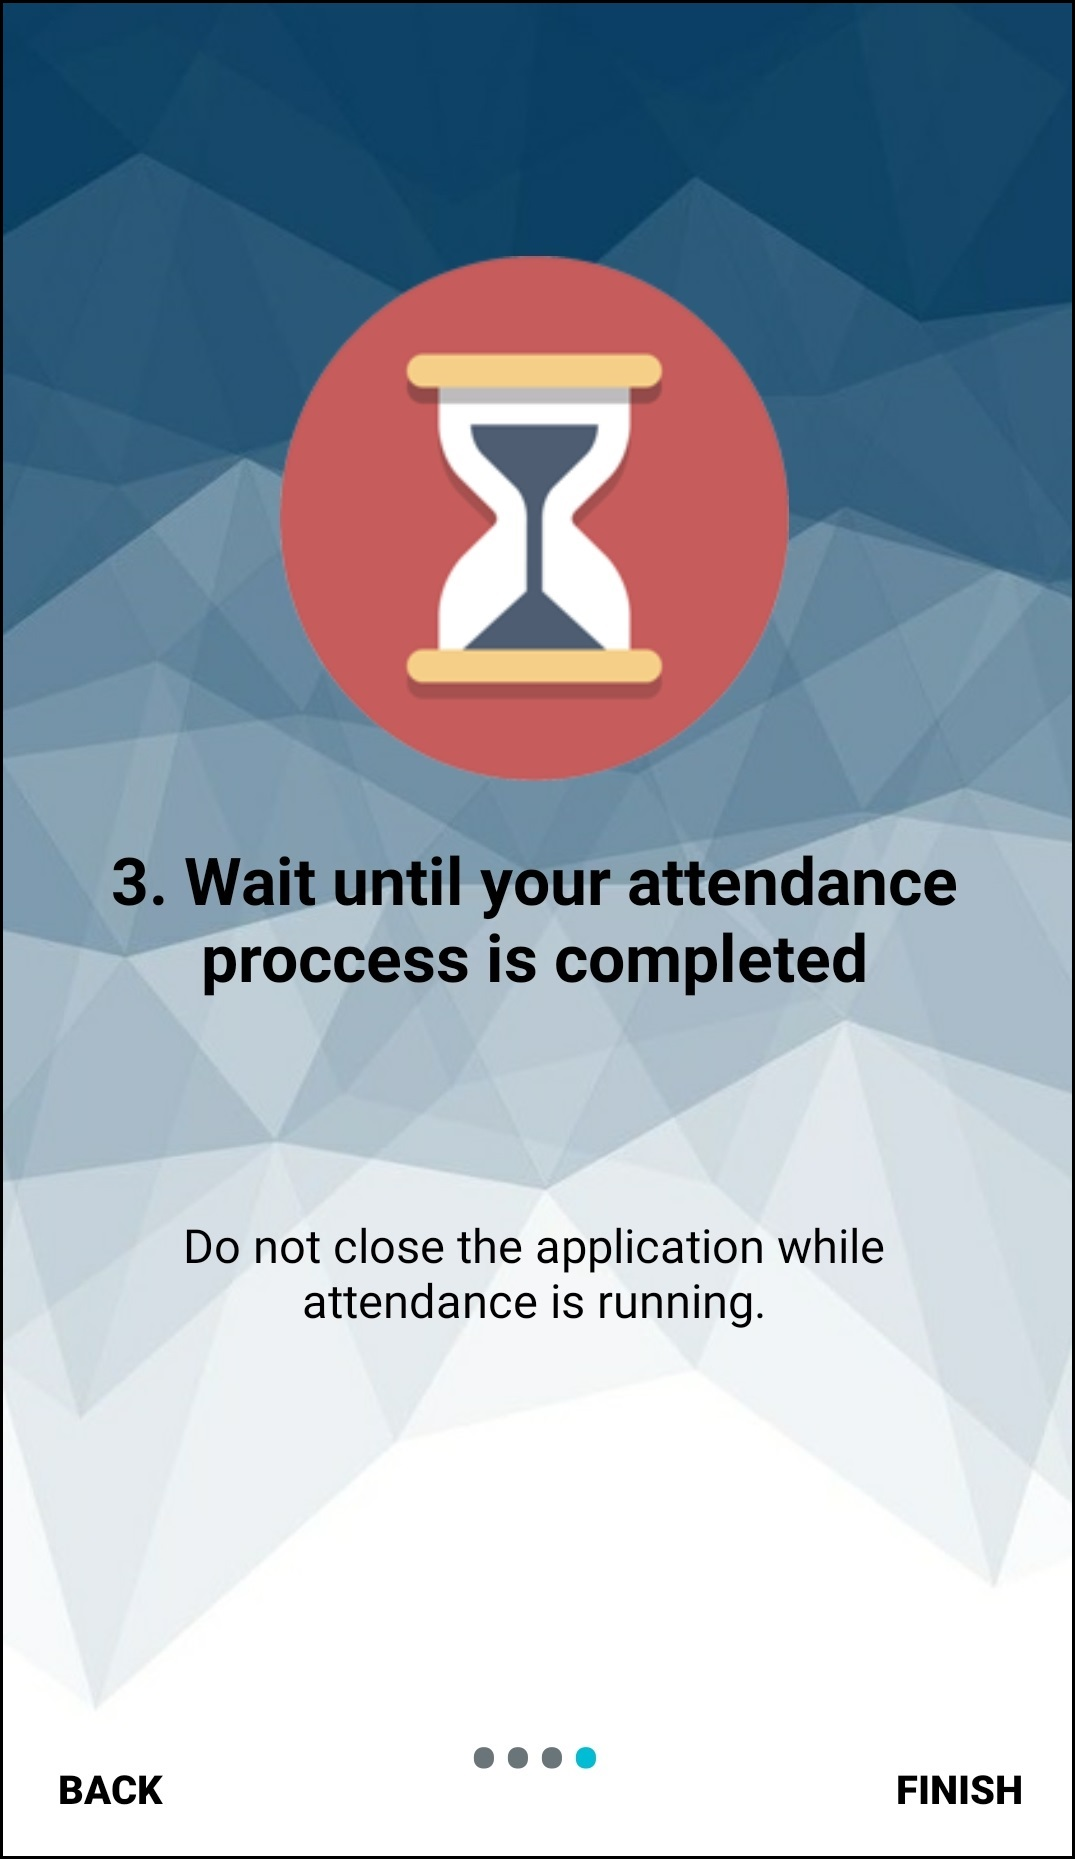
\includegraphics[width=.5\linewidth]{gambar/android/dosen-1}  
  		\caption{\textit{Landing page}}
	\end{subfigure}
	\begin{subfigure}{.5\textwidth}
  		\centering
  		% include second image
		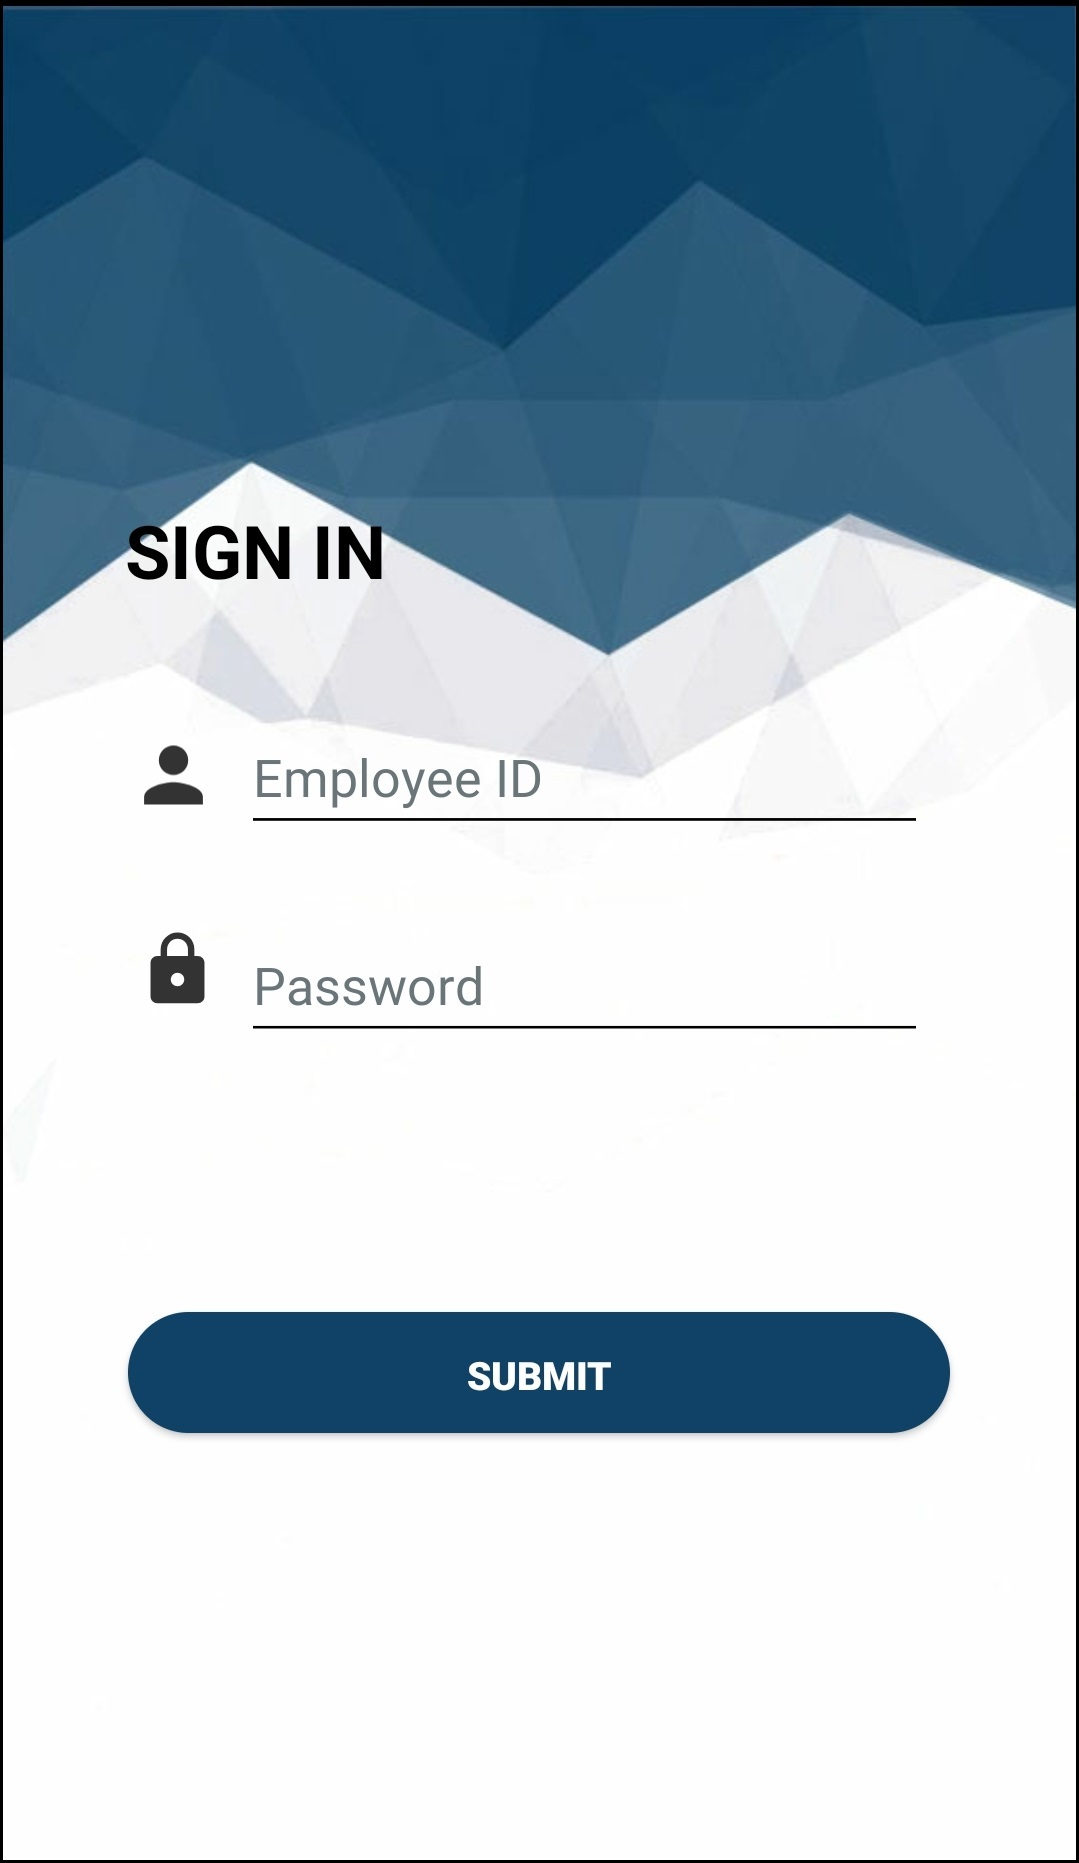
\includegraphics[width=.5\linewidth]{gambar/android/dosen-2}  
  		\caption{\textit{Log in}}
	\end{subfigure}
		\vspace{1cm}
		\newline
	\begin{subfigure}{.5\textwidth}
  		\centering
		 % include third image
	  	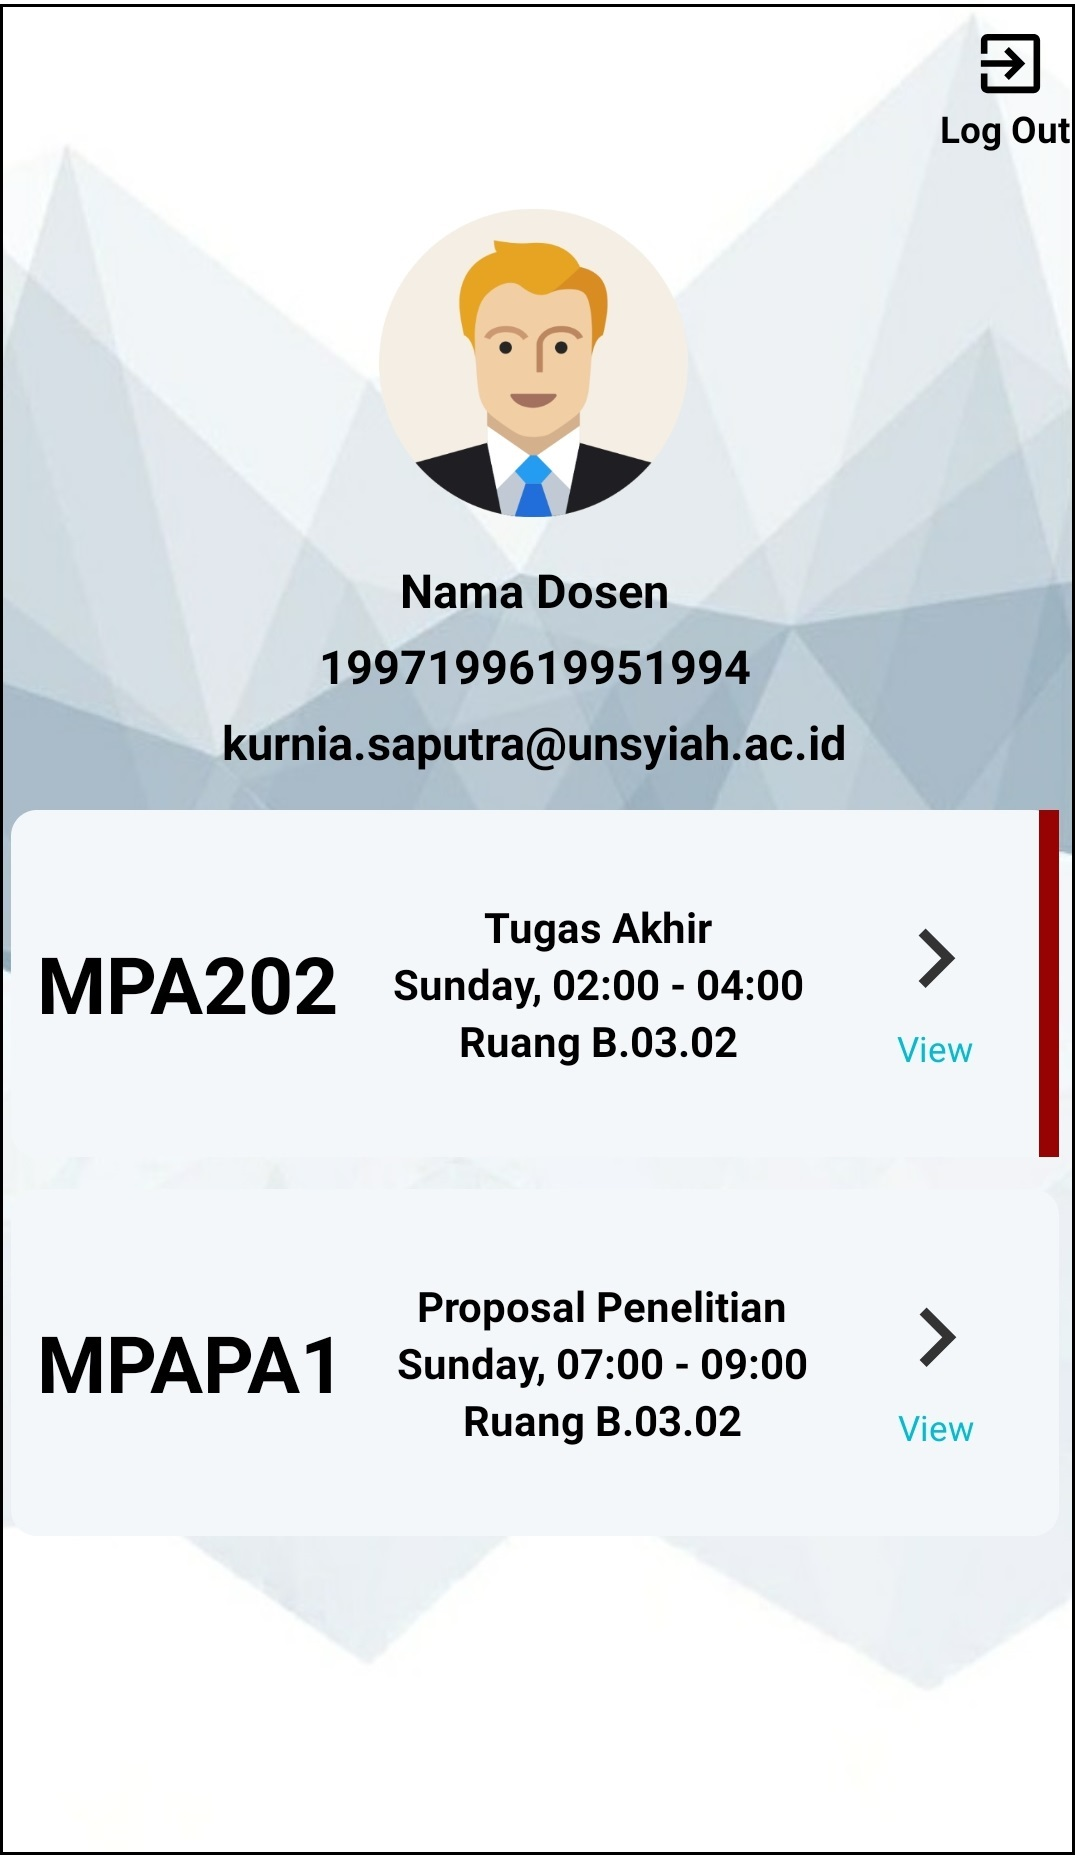
\includegraphics[width=.5\linewidth]{gambar/android/dosen-3}  
  		\caption{Beranda}
	\end{subfigure}
	\begin{subfigure}{.5\textwidth}
  		\centering
  		% include fourth image
  		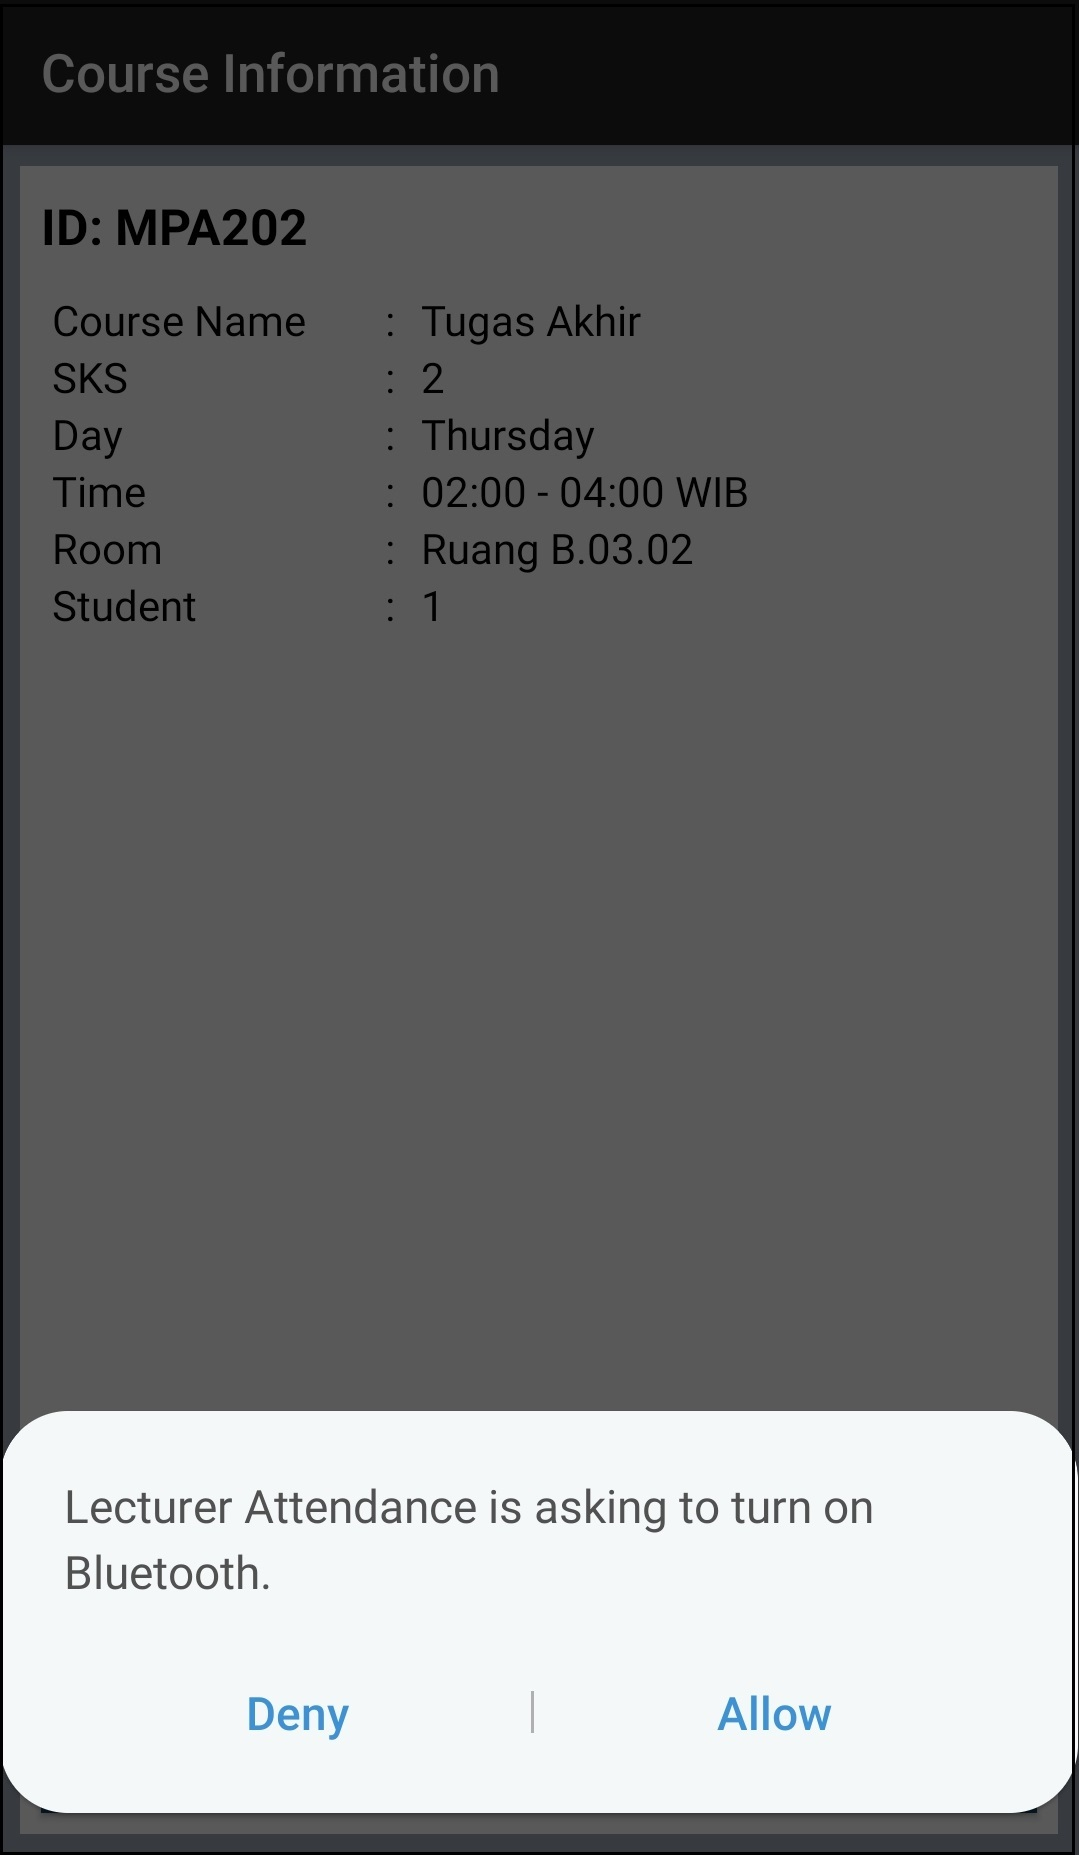
\includegraphics[width=.5\linewidth]{gambar/android/dosen-4}  
  		\caption{Informasi matakuliah}
	\end{subfigure}
		\vspace{0.5cm}
		\caption{Tampilan Halaman Aplikasi Kehadiran Dosen (Bagian 1)}
	\label{aplikasidosenbagian1}
	\end{figure}
	
\vspace{0.5cm}
	\par Gambar \ref{aplikasidosenbagian2} memperlihatkan ketika dosen telah berada di halaman informasi mata kuliah Kemudian, aplikasi akan menampilkan notifikasi untuk menghidupkan Bluetooth apabila Bluetooth pada perangkat belum hidup. Terdapat dua tombol yaitu tombol \textbf{show students} untuk melihat daftar mahasiswa yang mengambil mata kuliah tersebut dan tombol \textbf{start attendance} untuk memulai proses kehadiran. Aplikasi akan melakukan klasifikasi dengan metode K-NN untuk memprediksi lokasi dosen.
	
	\vspace{-0cm}
	\begin{figure} [H]
	\begin{subfigure}{.5\textwidth}
  		\centering
  		% include first image
  		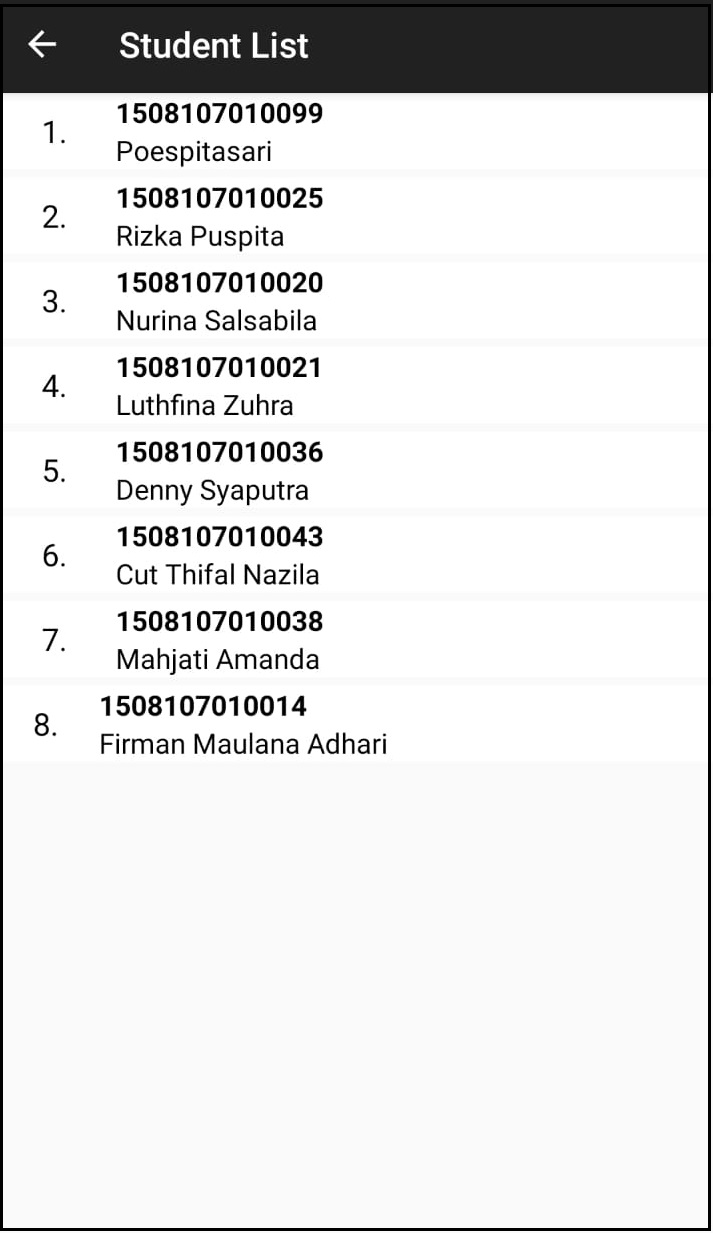
\includegraphics[width=.5\linewidth]{gambar/android/dosen-5}  
  		\caption{Daftar mahasiswa}
	\end{subfigure}
	\begin{subfigure}{.5\textwidth}
  		\centering
  		% include second image
  		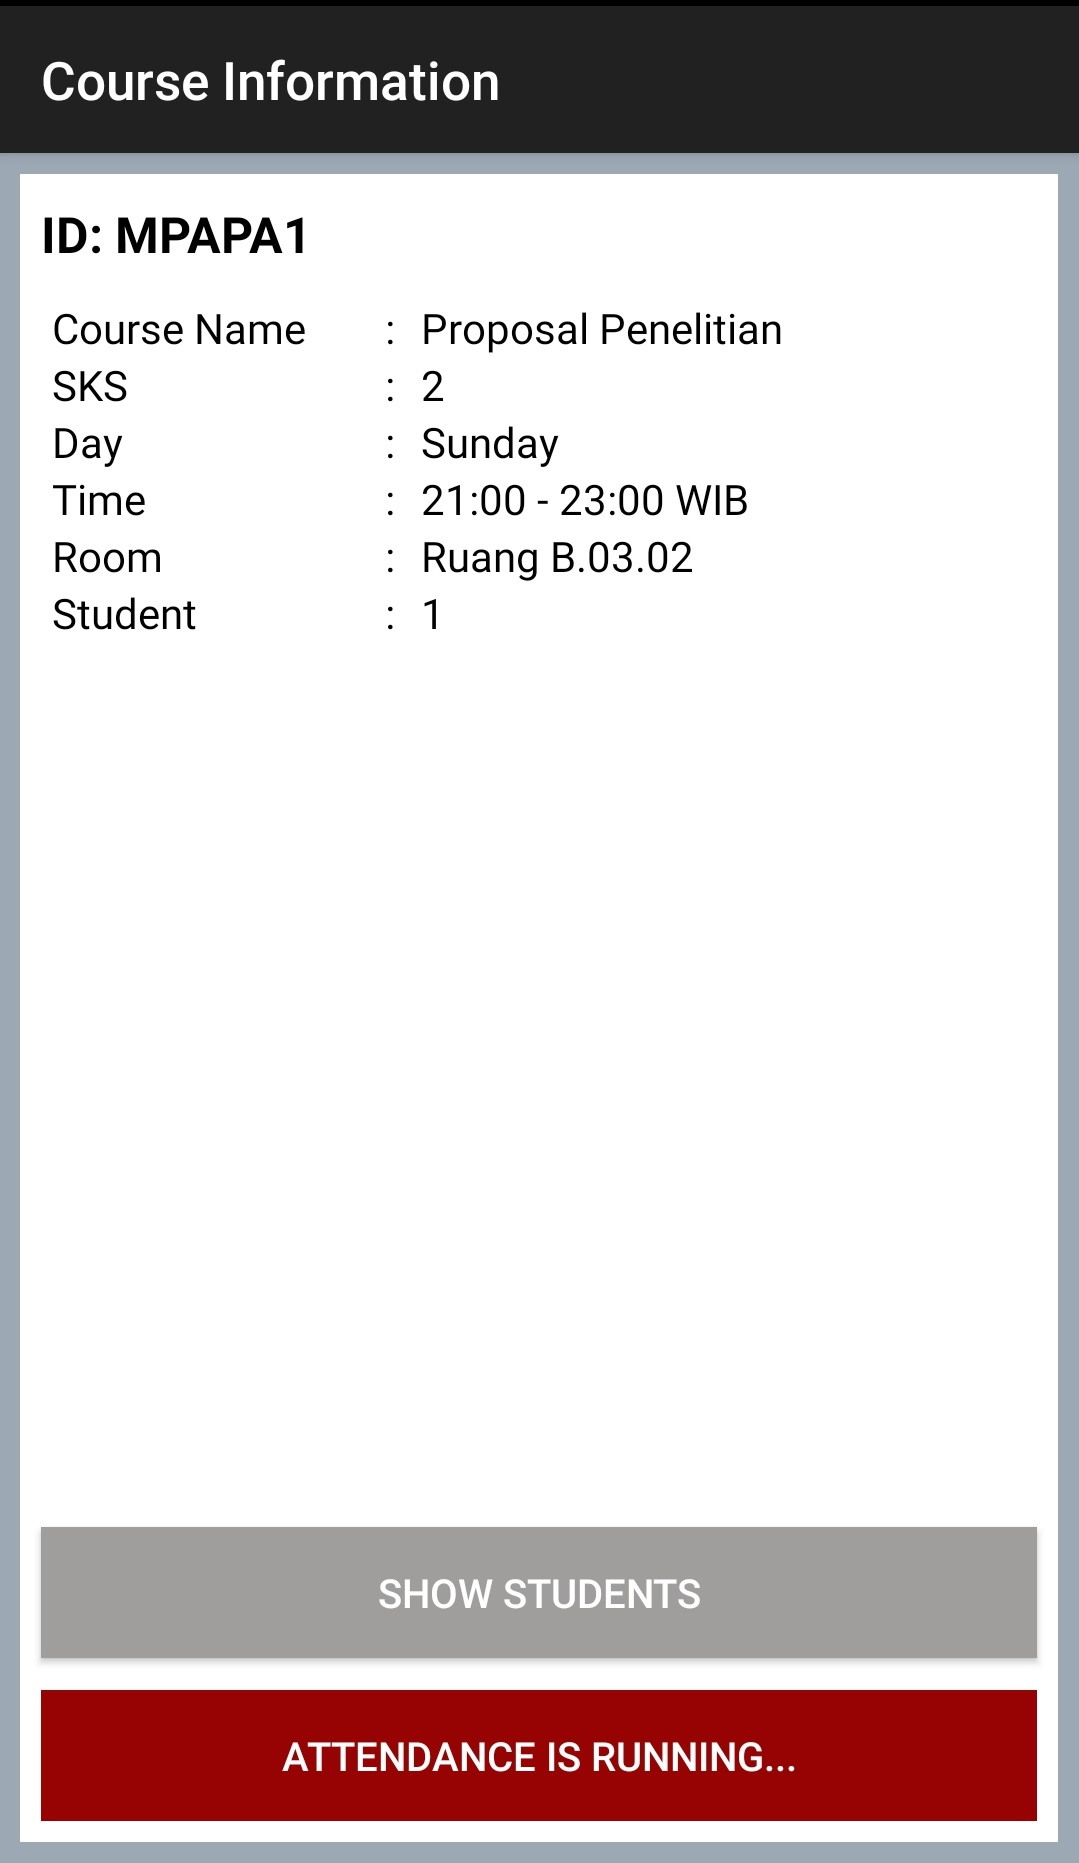
\includegraphics[width=.5\linewidth]{gambar/android/dosen-6}  
  		\caption{Proses kehadiran sedang berjalan}
	\end{subfigure}
	\vspace{1cm}
	\newline
	\begin{subfigure}{.5\textwidth}
  		\centering
  		% include third image
  		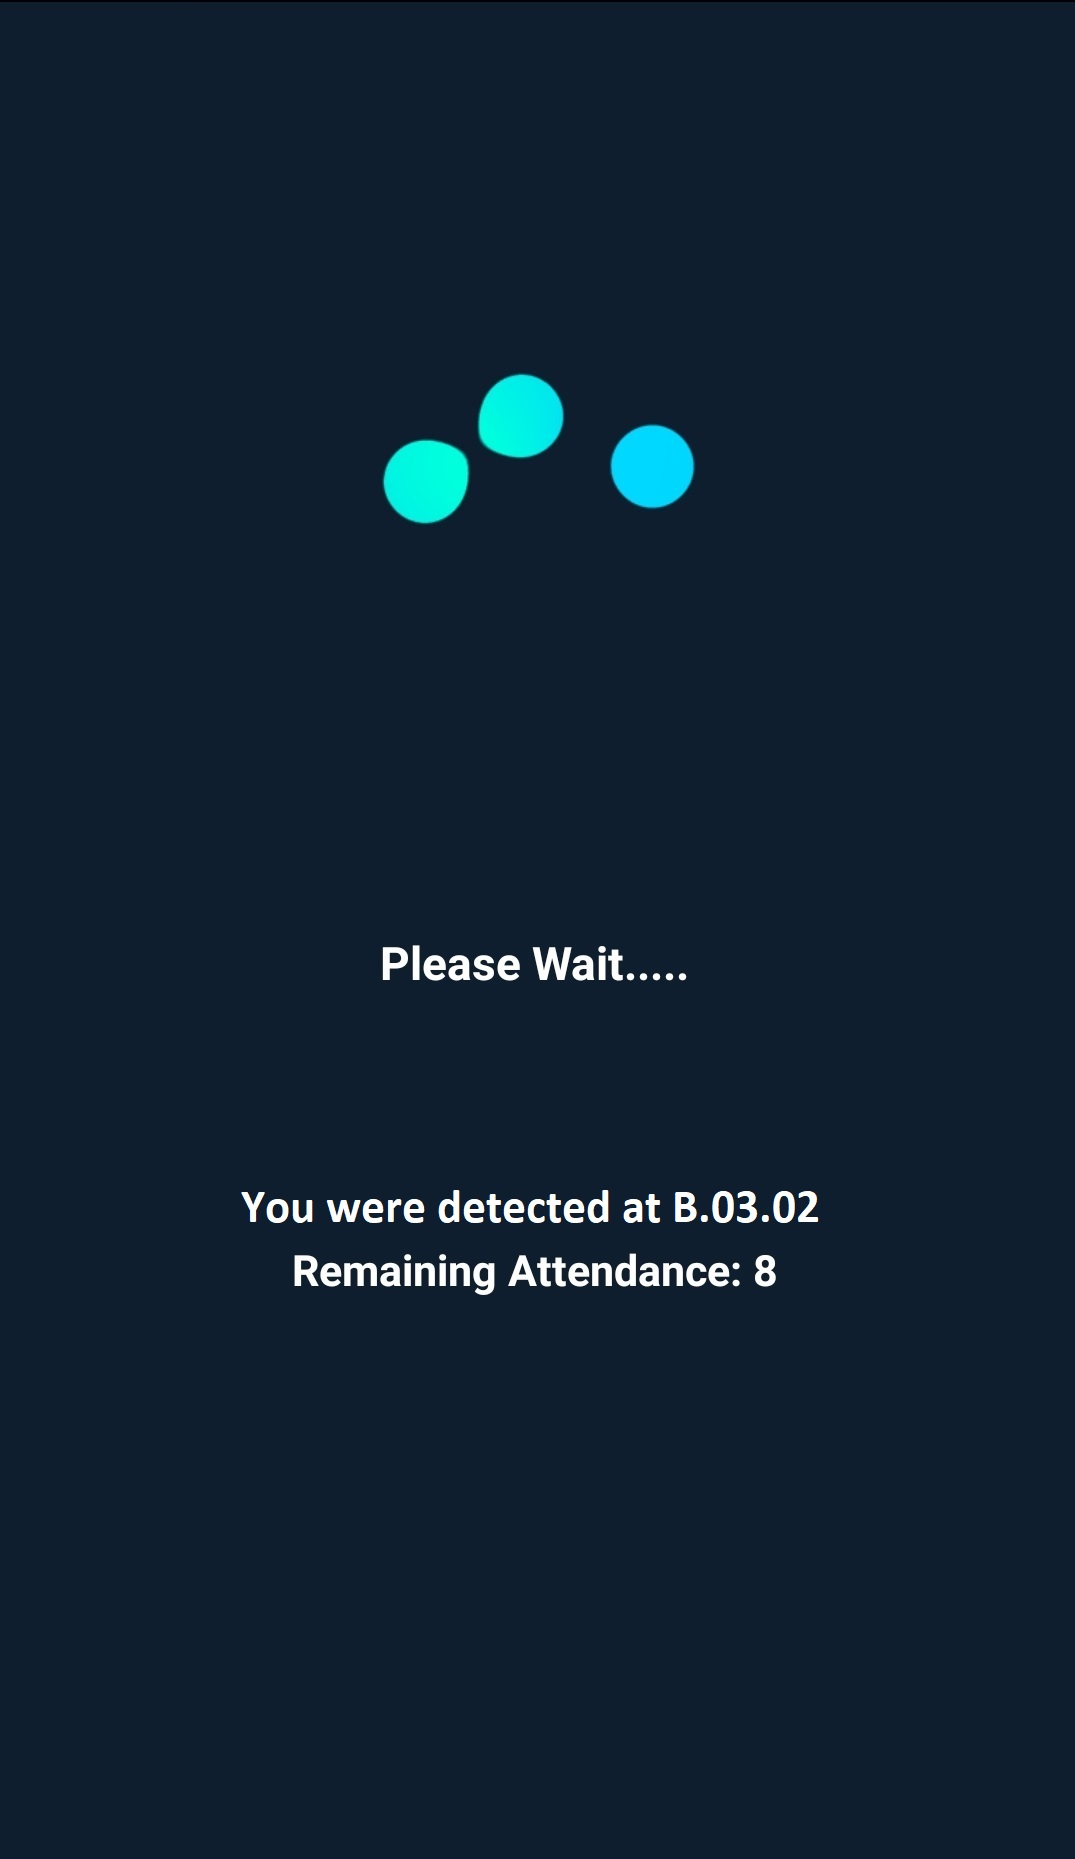
\includegraphics[width=.5\linewidth]{gambar/android/dosen-7}  
  		\caption{Dosen diprediksi di dalam kelas}
	\end{subfigure}
	\begin{subfigure}{.5\textwidth}
  		\centering
  		% include fourth image
  		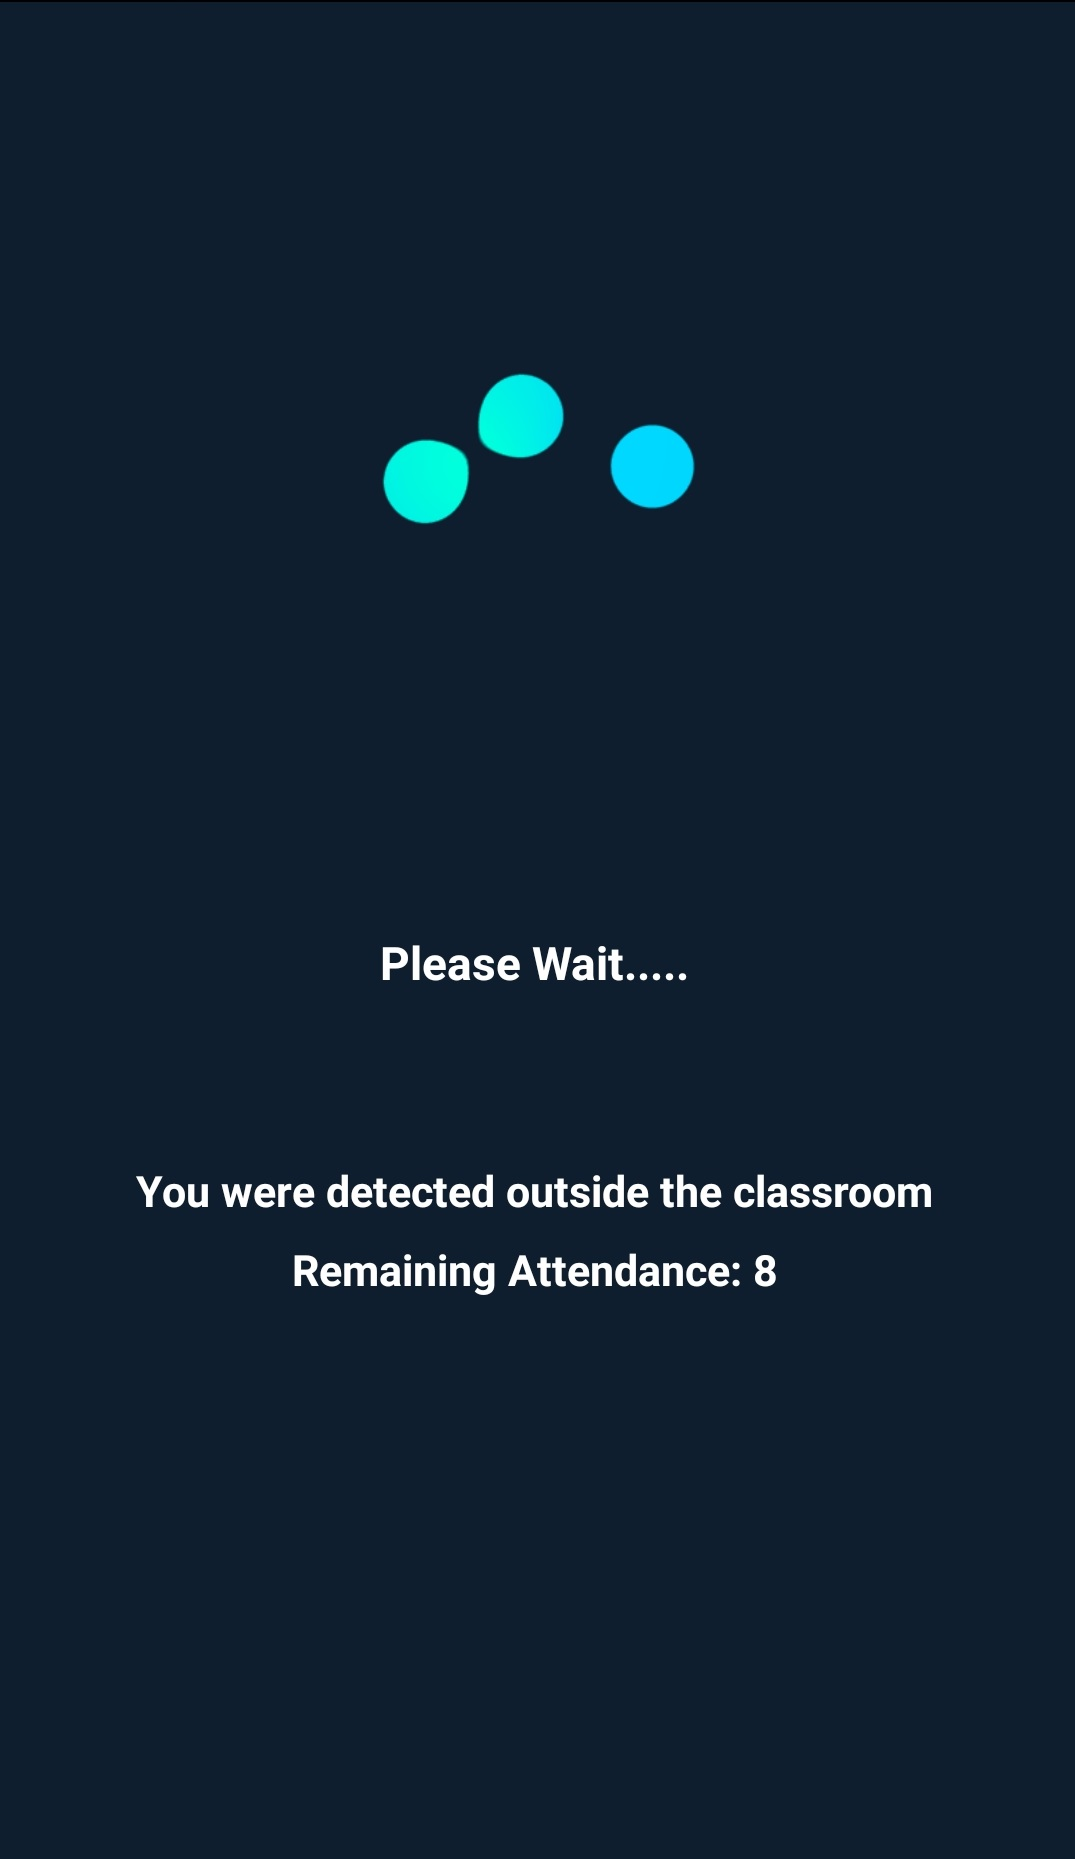
\includegraphics[width=.5\linewidth]{gambar/android/dosen-8}  
  		\caption{Dosen diprediksi di luar kelas}
	\end{subfigure}
		\vspace{0.5cm}
		\caption{Tampilan Halaman Aplikasi Kehadiran Dosen (Bagian 2)}
	\label{aplikasidosenbagian2}
	\end{figure}
	%Akhir Gambar Aplikasi Kehadiran Dosen%
	
	\item Antar Muka Aplikasi Kehadiran Mahasiswa
	
	\par Gambar \ref{aplikasimahasiswabagian1} memperlihatkan ketika mahasiswa belum melakukan \textit{log in}, aplikasi akan menampilkan \textit{landing page} yang berisi langkah-langkah penggunaan aplikasi, lalu mahasiswa akan diarahkan ke halaman \textit{log in}. Untuk melakukan \textit{log in}, mahasiswa diminta untuk memasukkan Nomor Pokok Mahasiswa (NPM) dan kata sandi yang sesuai dengan KRS Online Unsyiah. Setelah itu, mahasiswa akan diarahkan ke halaman beranda apabila telah berhasil melakukan \textit{log in}. Pada halaman beranda, terdapat beberapa menu seperti menu profil, menu daftar mata kuliah dan menu tentang aplikasi, serta informasi mata kuliah hari ini. 
	
	\vspace{-0cm}
	\begin{figure} [H]
	\begin{subfigure}{.5\textwidth}
  		\centering
  		% include first image
  		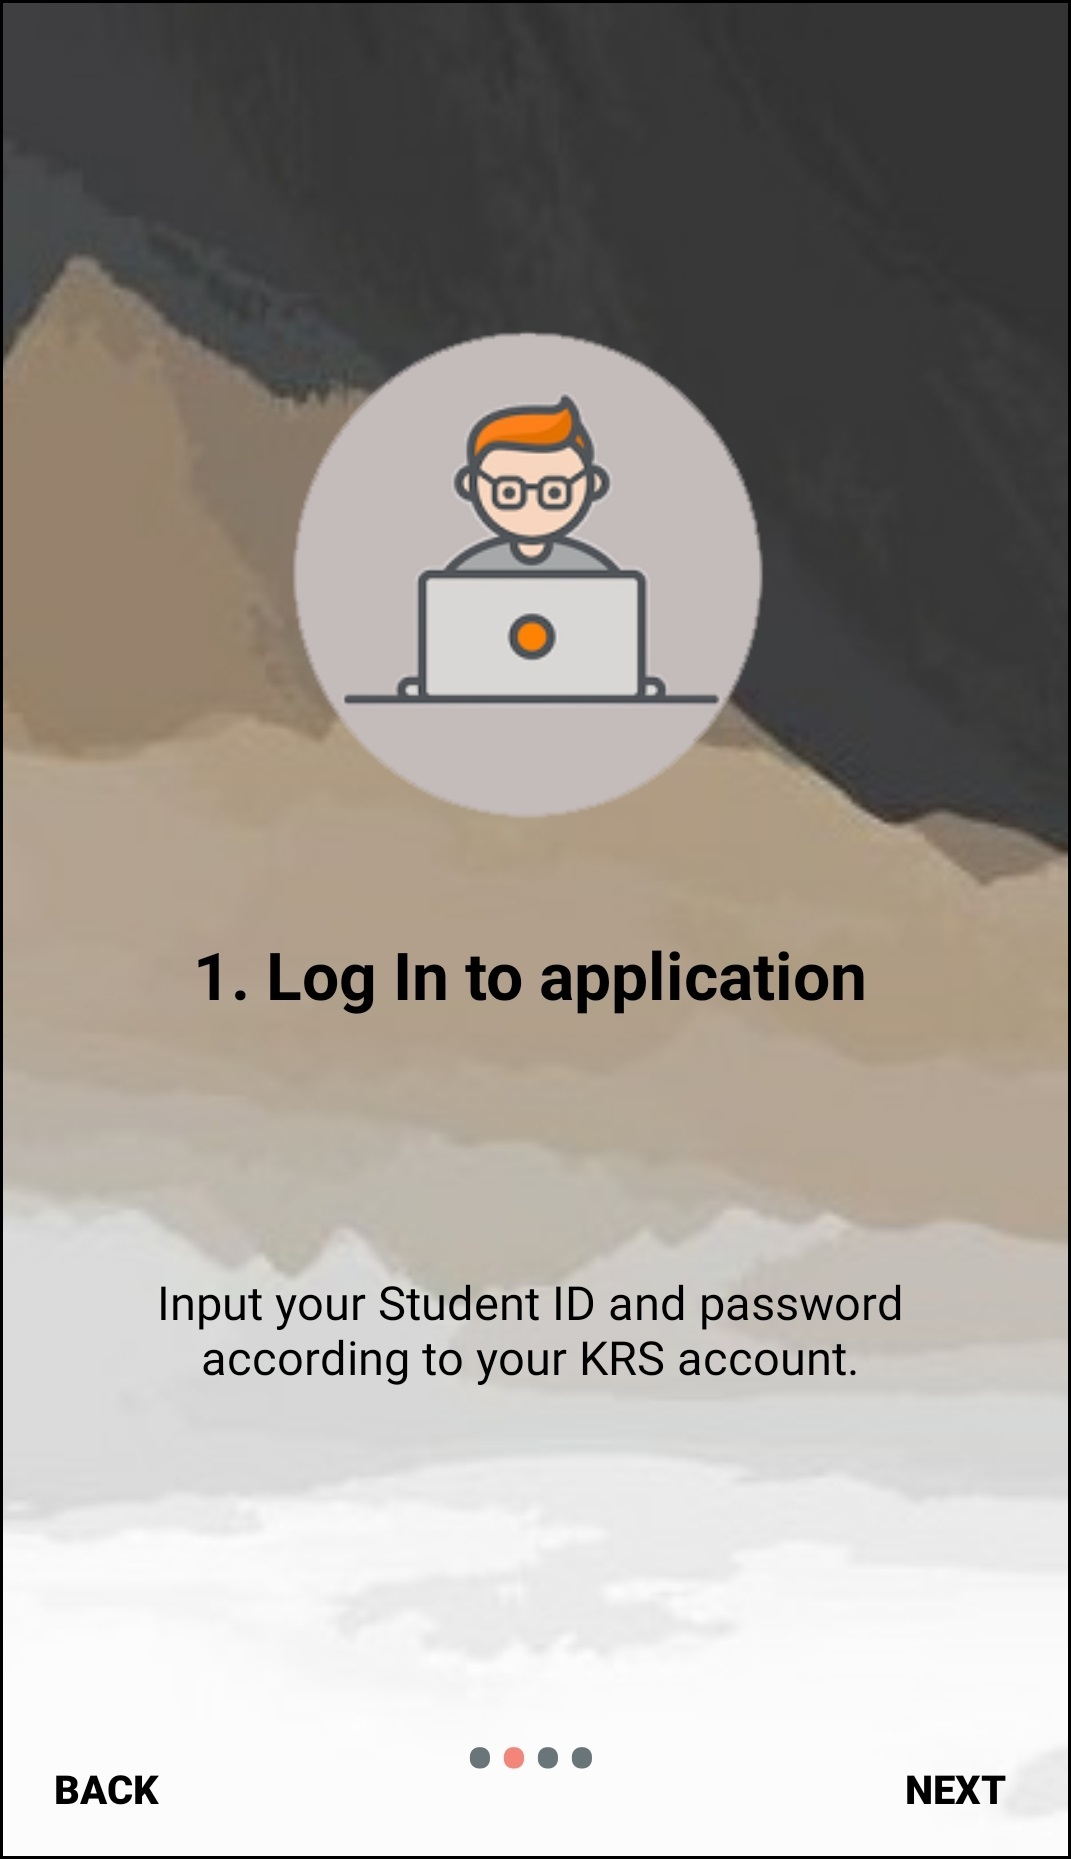
\includegraphics[width=.5\linewidth]{gambar/android/mahasiswa-1}  
  		\caption{\textit{Landing page}}
	\end{subfigure}
	\begin{subfigure}{.5\textwidth}
  		\centering
  		% include second image
  		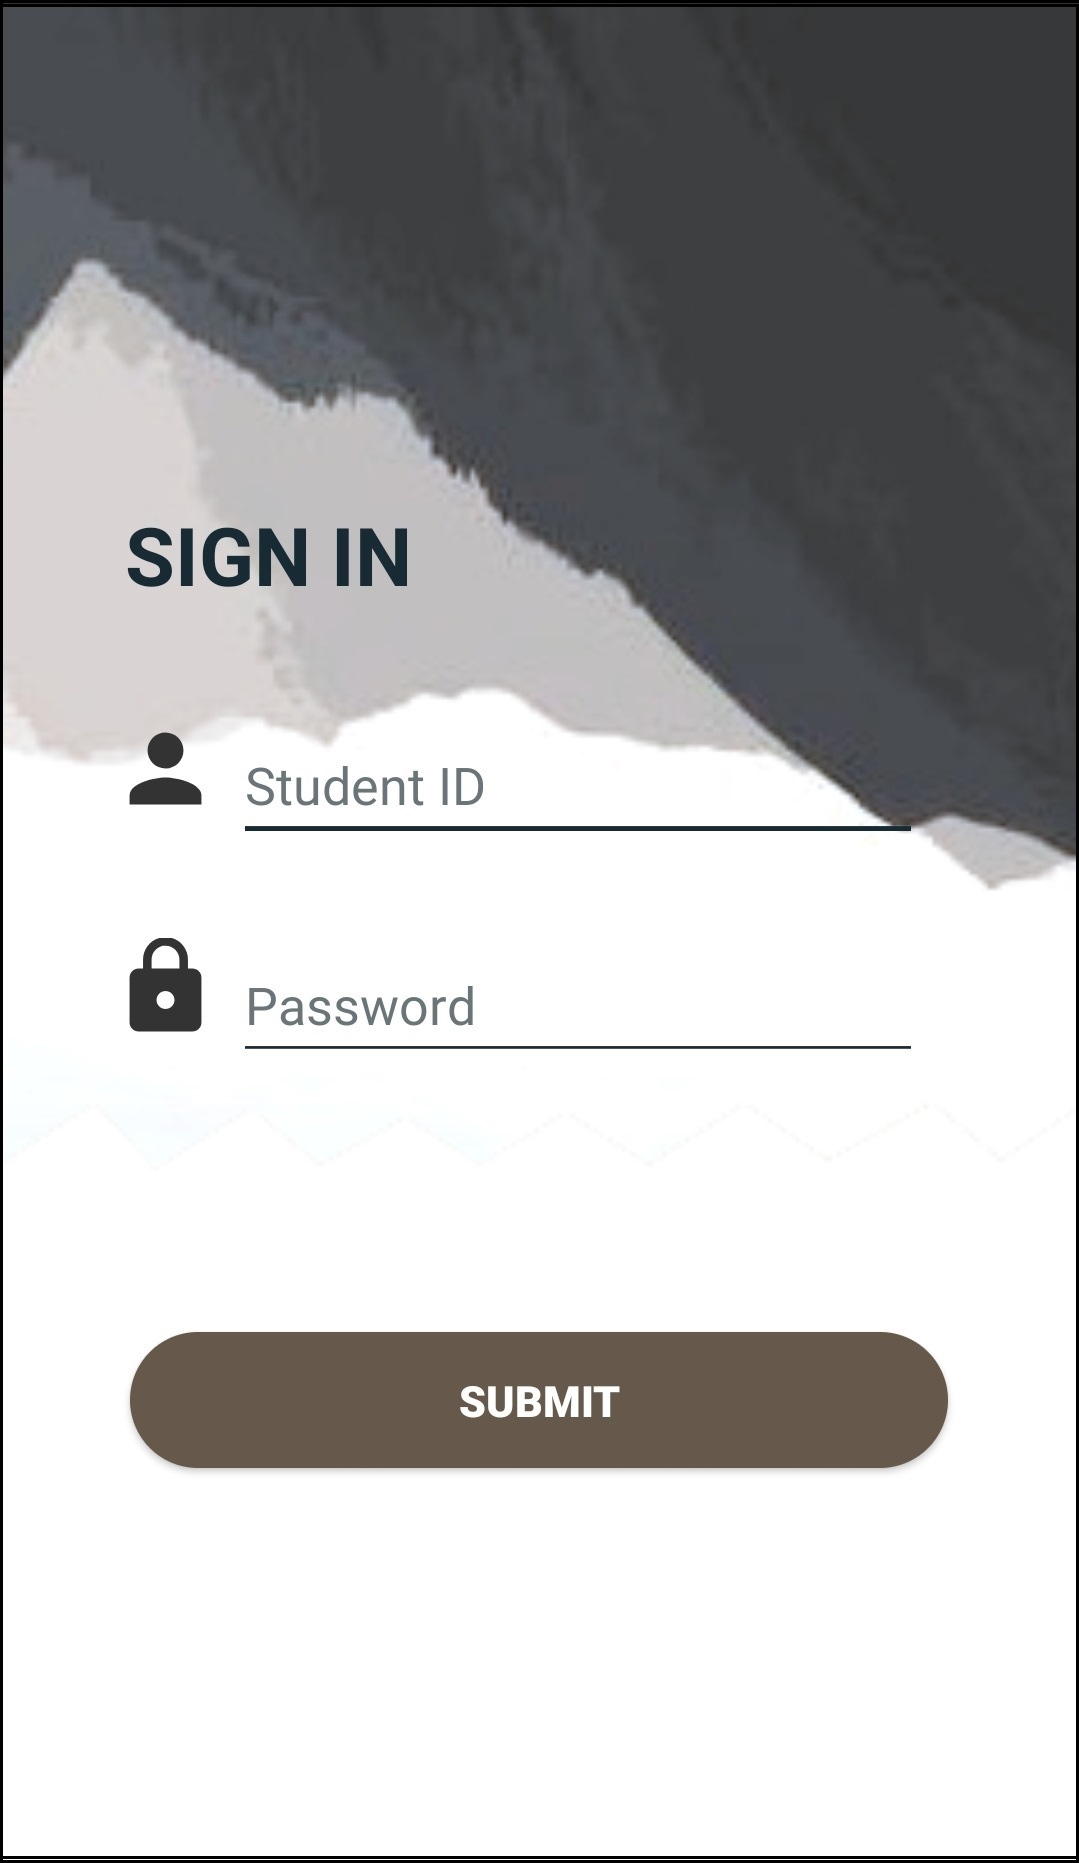
\includegraphics[width=.5\linewidth]{gambar/android/mahasiswa-2}  
  		\caption{\textit{Log in}}
	\end{subfigure}
	\vspace{1cm}
	\newline
	\begin{subfigure}{.5\textwidth}
  		\centering
  		% include third image
  		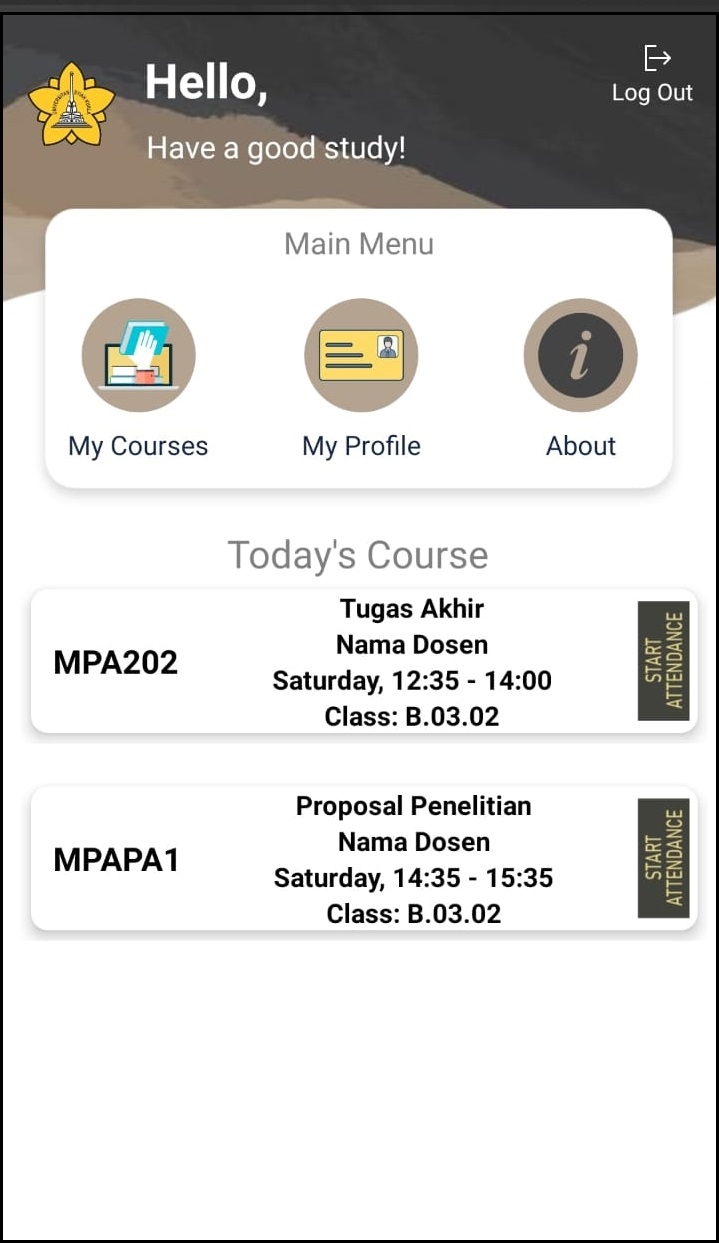
\includegraphics[width=.5\linewidth]{gambar/android/mahasiswa-3}  
  		\caption{Beranda}
	\end{subfigure}
	\begin{subfigure}{.5\textwidth}
  		\centering
  		% include fourth image
  		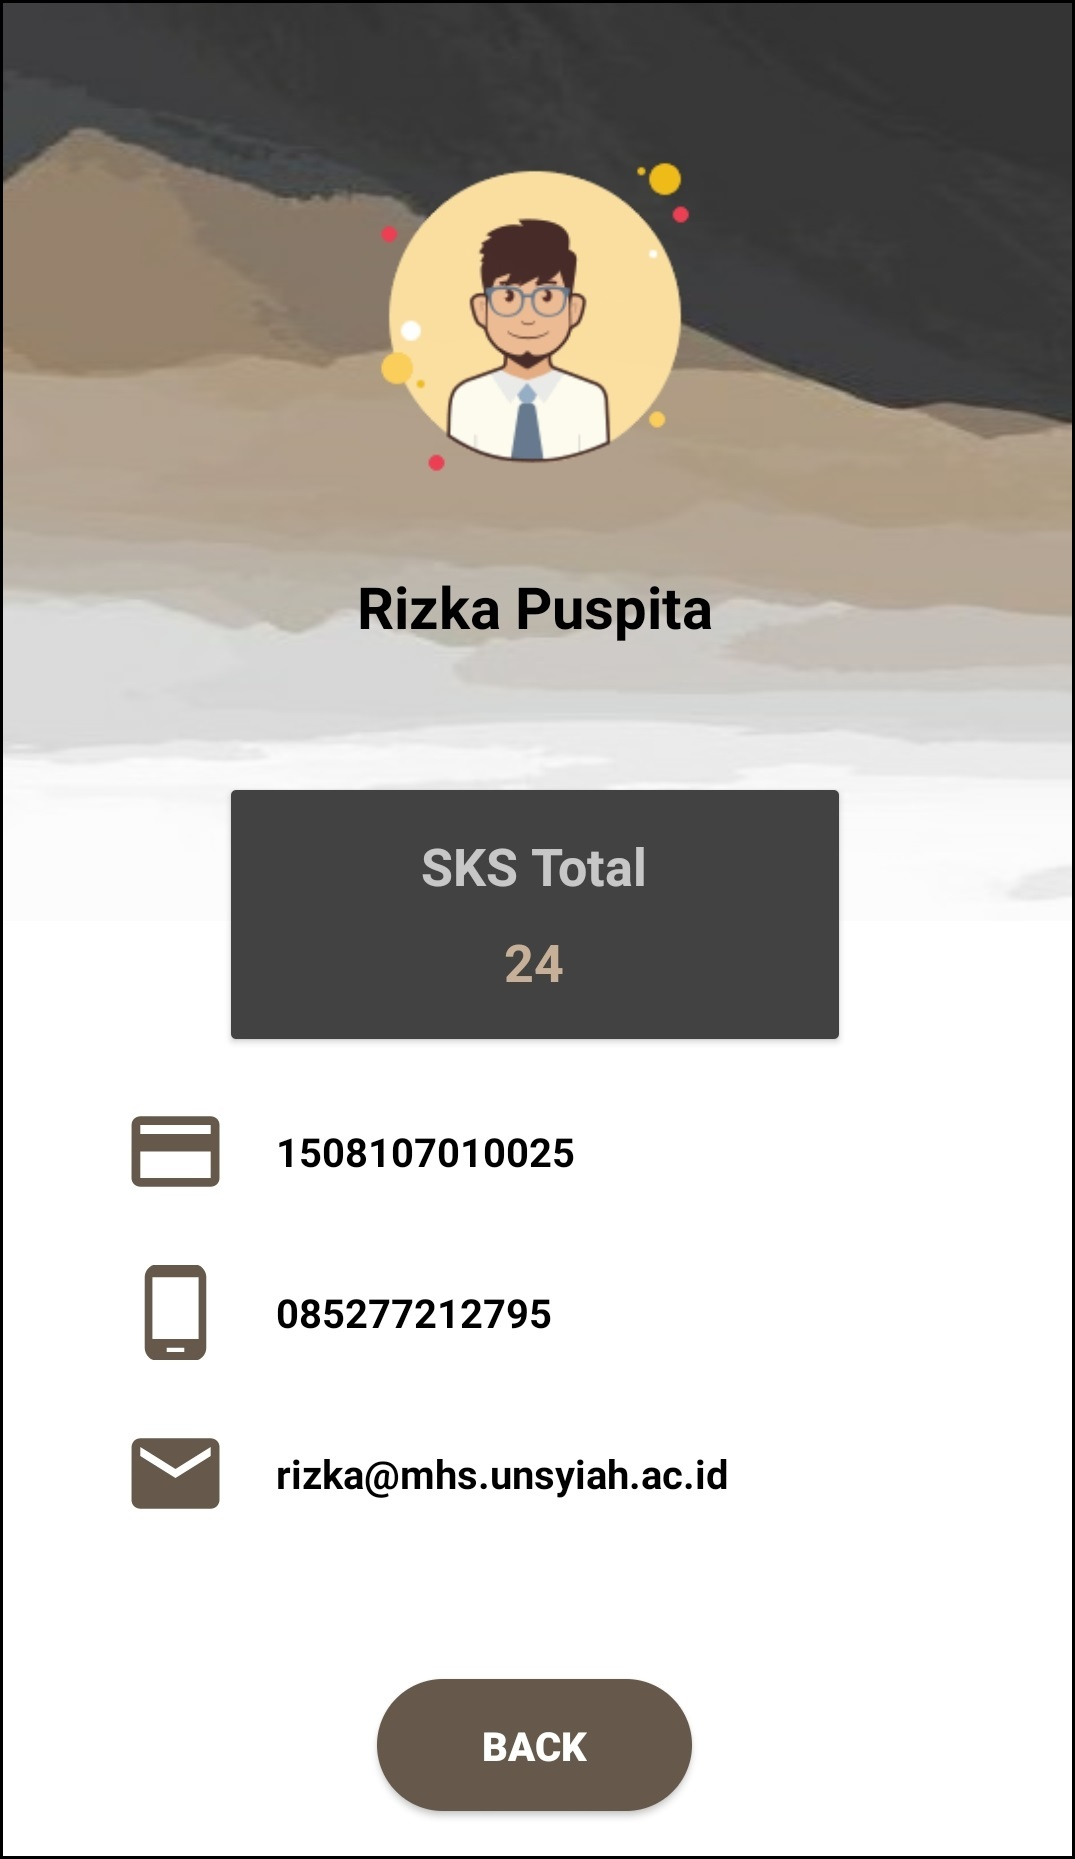
\includegraphics[width=.5\linewidth]{gambar/android/mahasiswa-4}  
  		\caption{Profil}
	\end{subfigure}
		\vspace{0.5cm}
		\caption{Tampilan Halaman Aplikasi Kehadiran Mahasiswa (Bagian 1)}
	\label{aplikasimahasiswabagian1}
	\end{figure}
	
		\par Gambar \ref{aplikasimahasiswabagian1} memperlihatkan daftar mata kuliah yang diambil oleh mahasiswa. Apabila mahasiswa menekan salah satu daftar mata kuliah, aplikasi akan memulai proses kehadiran yang dipicu oleh dosen ketika dosen telah memulai proses kehadiran. Kemudian, aplikasi akan menampilkan notifikasi untuk menghidupkan Bluetooth apabila Bluetooth pada perangkat belum hidup. Jika Bluetooth telah dihidupkan, aplikasi akan melakukan pencatatan kehadiran secara \textit{background proccess} sampai waktu matakuliah berakhir. Aplikasi akan melakukan klasifikasi dengan metode K-NN untuk memprediksi lokasi mahasiswa seperti yang terlihat pada Gambar \ref{aplikasimahasiswabagian2}.
		
	\vspace{-0cm}
	\begin{figure} [H]
	\begin{subfigure}{.5\textwidth}
  		\centering
  		% include first image
  		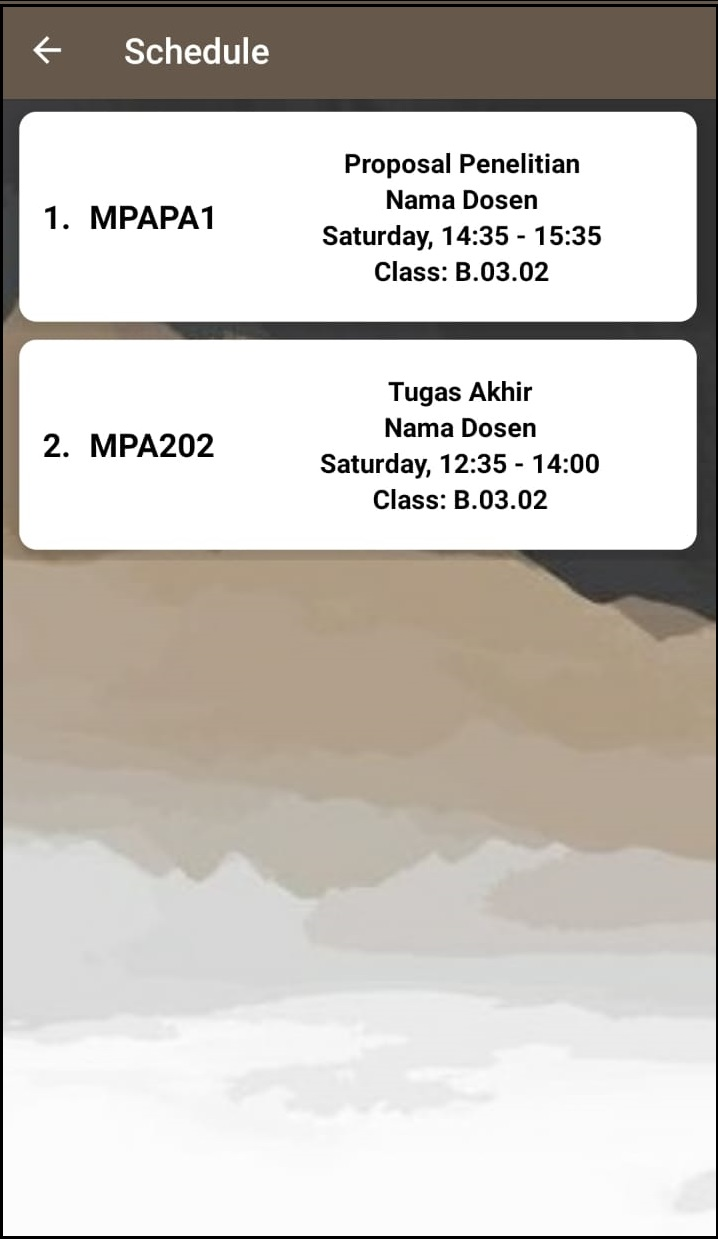
\includegraphics[width=.5\linewidth]{gambar/android/mahasiswa-5}  
  		\caption{Daftar mata kuliah}
	\end{subfigure}
	\begin{subfigure}{.5\textwidth}
  		\centering
  		% include second image
  		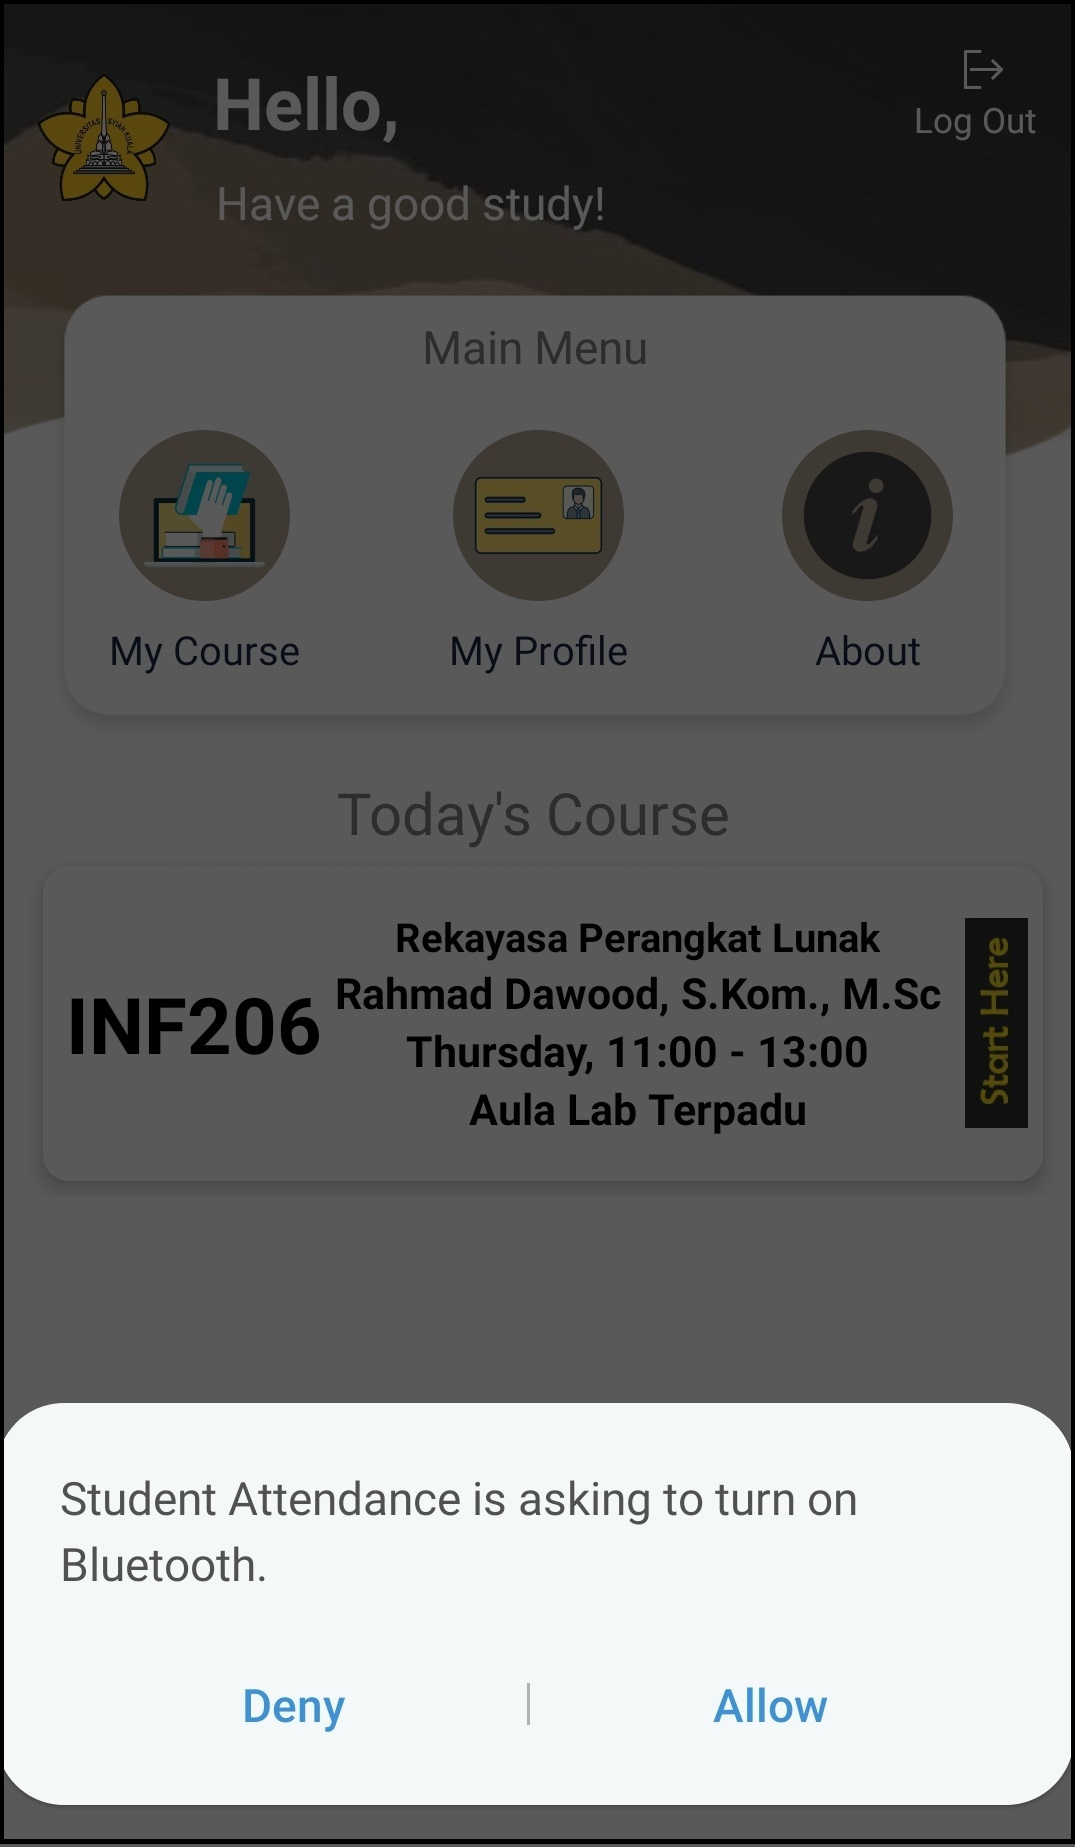
\includegraphics[width=.5\linewidth]{gambar/android/mahasiswa-6}  
  		\caption{Memulai proses kehadiran}
	\end{subfigure}
	\vspace{1cm}
	\newline
	\begin{subfigure}{.5\textwidth}
  		\centering
  		% include third image
  		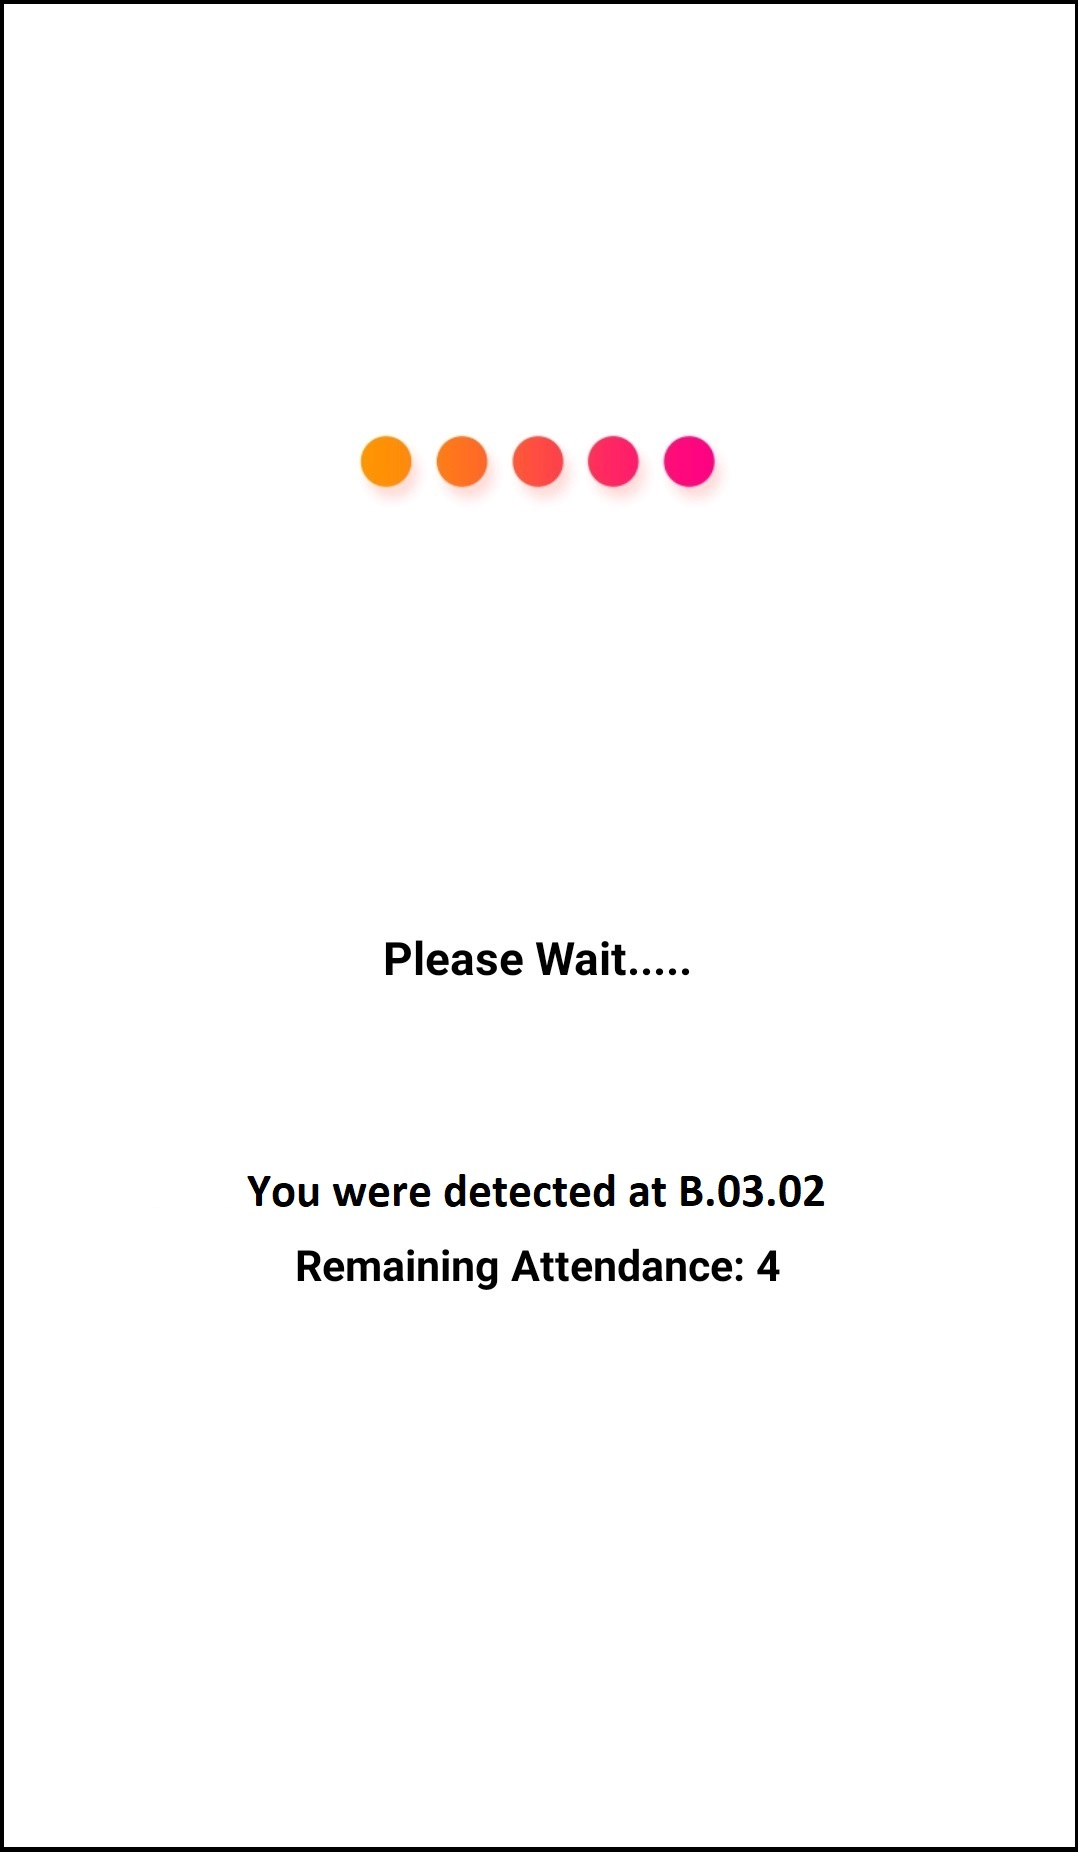
\includegraphics[width=.5\linewidth]{gambar/android/mahasiswa-7}  
  		\caption{Mahasiswa diprediksi di dalam kelas}
	\end{subfigure}
	\begin{subfigure}{.5\textwidth}
  		\centering
  		% include fourth image
  		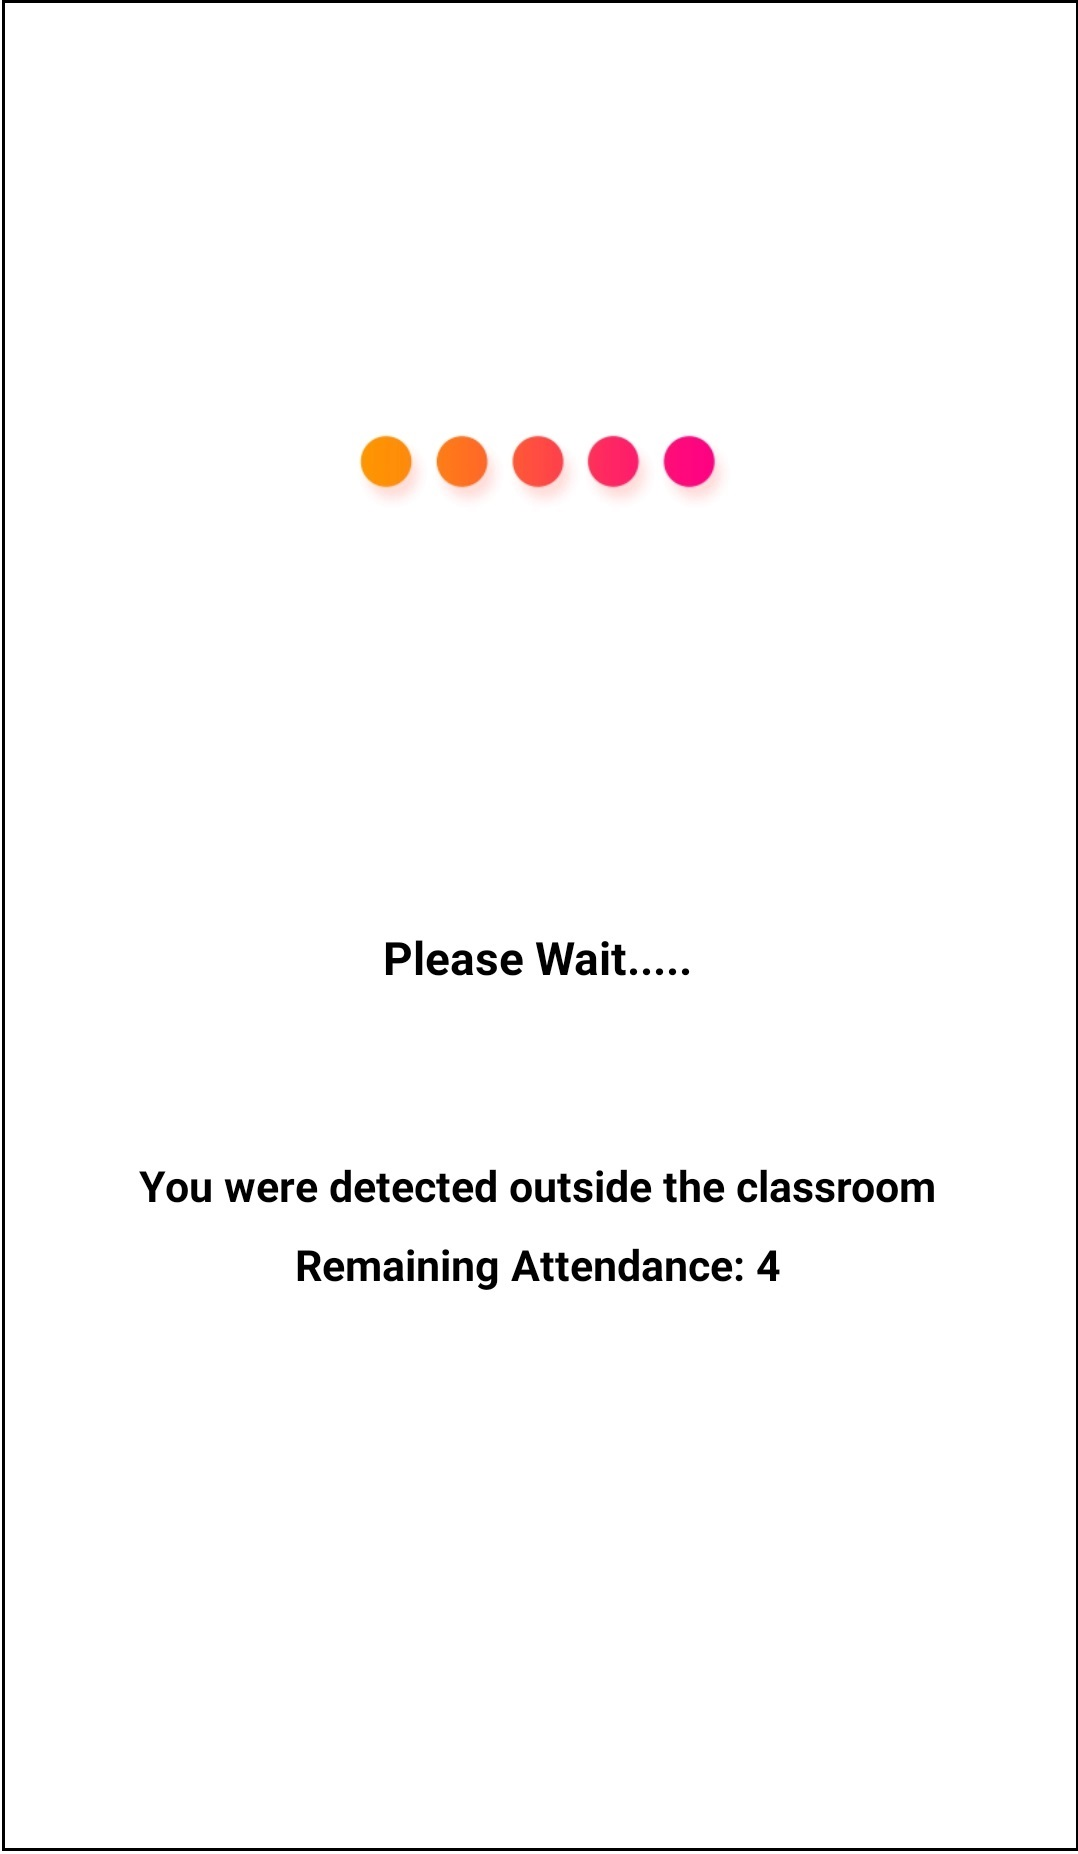
\includegraphics[width=.5\linewidth]{gambar/android/mahasiswa-8}  
  		\caption{Mahasiswa diprediksi di luar kelas}
	\end{subfigure}
		\vspace{0.5cm}
		\caption{Tampilan Halaman Aplikasi Kehadiran Mahasiswa (Bagian 2)}
	\label{aplikasimahasiswabagian2}
	\end{figure}

	%Akhir Gambar Aplikasi Kehadiran Mahasiswa%
	
		\end{enumerate}
		
%%%%%%%%%%%%%%%%%%%%%%%%%%%%%%%%%%%%%%%%%%%akhir perancangan aplikasi mapping%%%%%%%%%%%%%%%%%%%%%%%%%%%%%%%%%%%%%%%%%%%%%%%%%%%
	\subsection{Pembuatan Sistem}
	
	\begin{enumerate}[a.]
		\item Aplikasi Mapping
		\\ Aplikasi \textit{mobile} berbasis Android yang dikembangkan menggunakan bahasa pemrograman Java dengan bantuan IDE Android Studio. Media penyimpanan basis data pada aplikasi ini menggunakan SQLite. SQLite merupakan media penyimpanan lokal untuk setiap aplikasi yang sudah terpasang di perangkat Android, dikarenakan aplikasi ini hanya perlu menyimpan data-data hasil pemindaian kekuatan sinyal Bluetooth. Aplikasi mapping ini juga sudah memiliki sertifikat Hak Kekayaan Intelektual (HKI) dengan nomor EC00201972853 yang dapat dilihat pada lampiran 1. Potongan kode program untuk melakukan pemindaian kekuatan sinyal Bluetooth dapat dilihat pada Program 4.1 berikut ini.
		\vspace{0.4cm}
			\lstset{language=Java,
			basicstyle=\ttfamily\scriptsize\color{black},
			keywordstyle=\color{javapurple}\bfseries,
			stringstyle=\color{javared},
			commentstyle=\color{javagreen},
			morecomment=[s][\color{javadocblue}]{/**}{*/},
			numbers=left,
			numberstyle=\tiny\color{black},
			showstringspaces=false,
			numbersep=10pt,
			tabsize=4,
			showspaces=false,
			showstringspaces=false,
			autogobble=true,
			xleftmargin=2em
		}
	\begin{lstlisting}[label=programScanBle]
    private HashMap<String, BTLEDevice> mBTDevicesHashMap;
    private Ble pojoBle;

    mBTDevicesHashMap = new HashMap<>(); // membuat objek kelas HashMap.
	
	/**
     * @param device parameter dari kelas BluetoothDevice yang akan ditambahkan.
     * @param rssi rssi dari kelas BluetoothDevice.
     */
    public void addDevice(BluetoothDevice device, int rssi) {
     String address = device.getAddress();
      if (!mBTDevicesHashMap.containsKey(address)) {
         if (address.equals(pojoBle.ADDRESS_1) || address.equals(pojoBle.ADDRESS_2) 
             .... 
             || address.equals(pojoBle.ADDRESS_9));
         {
             BTLEDevice btleDevice = new BTLEDevice(device);
             btleDevice.setRSSI(rssi);
             mBTDevicesHashMap.put(address, btleDevice);
             mBTDevicesArrayList.add(btleDevice);
         }
      }
      else {
            mBTDevicesHashMap.get(address).setRSSI(rssi);
        }
    }
	\end{lstlisting}
	 \captionof{lstlisting}{Potongan Kode Program Membaca Informasi Bluetooth.}

		
		\item Aplikasi Kehadiran Dosen
		\\ Aplikasi \textit{mobile} berbasis Android yang dikembangkan menggunakan bahasa pemrograman Java dengan bantuan IDE Android Studio. Media penyimpanan aplikasi ini menggunakan basis data server yaitu MySQL. Basis data server tersebut diakses melalui REST server API yang dibangun menggunakan bahasa pemrograman PHP. Aplikasi ini bertindak sebagai klien. Oleh karena itu, aplikasi ini menggunakan \textit{library} Retrofit untuk melakukan \textit{request} ke server dan menghandle \textit{response} dalam bentuk JavaScript Object Notation (JSON). Proses pengiriman data dari klien ke server dilakukan ketika dosen menekan tombol \textbf{start attendance} pada aplikasi. %Potongan kode program yang dibuat untuk melakukan pengiriman data dapat dilihat pada kode \ref{programStartAbsen} berikut ini. 
		Seorang dosen dapat terhitung menghadiri perkuliahan pada aplikasi apabila syarat-syarat di bawah ini terpenuhi:
		\begin{enumerate}[1.]
		\item Dosen menekan tombol \textbf{start attendance} 50 menit sebelum mata kuliah berakhir. 
		\item Dosen menekan tombol \textbf{start attendance} sesuai waktu yang telah ditentukan. Penentuan lokasi dilakukan dengan menggunakan metode klasifikasi K-NN yang dapat dilihat pada Program 4.2 berikut ini.
		\vspace{0.4cm}
		% KODE KNN%
	\begin{lstlisting}[label=programKNNDosen]
	public void stopScan() {
    // ambil semua nilai yang ada di HashMap (Bluetooth yang terdeteksi).
     Set<String> keys = mBTDevicesHashMap.keySet();
     String empty = "";
     String sinyal = "";
     for(String key : keys ) {
         empty += mBTDevicesHashMap.get(key).getAddress()+"\n";
         sinyal += mBTDevicesHashMap.get(key).getRSSI()+"\n";
     }
     //inisialisasi lokasi file data training.
     String train = "data_training_sequence_point.csv";
     //untuk mengambil data hasil pemindaian yg tersimpan di Hash.
     BTLE_Device ble1 = mBTDevicesHashMap.get(Ble.ADDRESS_1);
     ....  
     BTLE_Device ble9 = mBTDevicesHashMap.get(Ble.ADDRESS_9);
     //untuk kasih nilai default apabila sinyal Bluetooth tidak dapat.
     int rssi1 = ble1 == null ? -110 : ble1.getRSSI();
     ....
     int rssi9 = ble9 == null ? -110 : ble9.getRSSI();
     double[] testData = {rssi1, rssi2, ..., rssi9};
      try {
          InputStream streamTrain = getAssets().open(train);
          label = (int) KNN.knn(streamTrain, testData, 5);
          boolean masukKelas = (label == idRuang);
      } catch (IOException e) {
          e.printStackTrace();
       	}
    }
    
    \end{lstlisting}
    \captionof{lstlisting}{Potongan Kode Program Klasifikasi Metode K-NN Aplikasi Kehadiran Dosen.}

		\item Setiap mata kuliah memiliki satu sesi proses pencatatan kehadiran setiap 10 menit. Di setiap sesi tersebut, setiap aplikasi kehadiran dosen akan melakukan pencatatan kehadiran dengan pada waktu acak antara menit pertama hingga menit ke-10 setiap sesi. Sebagai contoh, mata kuliah A dimulai pada pukul 14:00 sampai pukul 16:00. Apabila satu sesi dilakukan per-10 menit sekali, maka total sesinya adalah 12 kali untuk proses pencatatan kehadiran. Misalnya sesi pertama dimulai pada pukul 14:02, pada saat itu aplikasi akan memprediksi lokasi dosen dan mengirimnya ke server untuk disesuaikan apakah kelas yang diprediksi saat itu sama dengan kelas sebenarnya. Jika prediksinya sesuai, maka dosen tersebut terhitung hadir. Kemudian, sesi kedua dimulai pada pukul 14:18. Jika prediksi yang dilakukan tidak sesuai, maka dosen tersebut terhitung tidak hadir. Proses tersebut akan berlangsung sampai sesi terakhir. Dari hasil prediksi setiap sesi tersebut, akan dihitung \textit{threshold} minimal 80\% dari jumlah proses pencatatan kehadiran yang dilakukan oleh aplikasi. 
		\end{enumerate}
		
		\vspace{0.5cm}
		\item Aplikasi Kehadiran Mahasiswa
		\\ Aplikasi \textit{mobile} berbasis Android yang dikembangkan menggunakan bahasa pemrograman Java dengan bantuan IDE Android Studio. Media penyimpanan aplikasi ini menggunakan basis data server yaitu MySQL. Basis data server tersebut diakses melalui REST server API yang dibangun menggunakan bahasa pemrograman PHP. Aplikasi ini bertindak sebagai klien. Oleh karena itu, aplikasi ini menggunakan \textit{library} Retrofit untuk melakukan \textit{request} ke server dan menghandle \textit{response} dalam bentuk JavaScript Object Notation (JSON). Proses pengiriman data dari klien ke server dilakukan ketika mahasiswa menekan tombol \textbf{start attendance} pada aplikasi. 
\newline
Seorang mahasiswa dapat terhitung menghadiri perkuliahan pada aplikasi apabila syarat-syarat di bawah ini terpenuhi:
		\begin{enumerate}[1.]
		\item Mahasiswa menekan tombol \textbf{start attendance} ketika perkuliahan sudah dimulai oleh dosen. Penentuan lokasi dilakukan dengan menggunakan metode klasifikasi K-NN yang dapat dilihat pada Program 4.3 berikut ini.
		\vspace{0.4cm}
		% KODE KNN%
	\begin{lstlisting}[label=programKNNMahasiswa]
	public void stopScan() {
    // ambil semua nilai yang ada di HashMap (Bluetooth yang terdeteksi).
     Set<String> keys = mBTDevicesHashMap.keySet();
     String empty = "";
     String sinyal = "";
     for(String key : keys ) {
         empty += mBTDevicesHashMap.get(key).getAddress()+"\n";
         sinyal += mBTDevicesHashMap.get(key).getRSSI()+"\n";
     }
     //inisialisasi lokasi file data training.
     String train = "data_training_sequence_point.csv";
     //untuk mengambil data hasil pemindaian yg tersimpan di Hash.
     BTLE_Device ble1 = mBTDevicesHashMap.get(Ble.ADDRESS_1);
     ....  
     BTLE_Device ble9 = mBTDevicesHashMap.get(Ble.ADDRESS_9);
     //untuk kasih nilai default apabila sinyal Bluetooth tidak dapat.
     int rssi1 = ble1 == null ? -110 : ble1.getRSSI();
     ....
     int rssi9 = ble9 == null ? -110 : ble9.getRSSI();
     double[] testData = {rssi1, rssi2, ..., rssi9};
      try {
          InputStream streamTrain = getAssets().open(train);
          label = (int) KNN.knn(streamTrain, testData, 5);
          boolean masukKelas = (label == idRuang);
      } catch (IOException e) {
          e.printStackTrace();
       	}
    }
    \end{lstlisting}
    \captionof{lstlisting}{Potongan Kode Program Klasifikasi Metode K-NN Aplikasi Kehadiran Mahasiswa.}
    
		\vspace{2cm}
		\item Setiap mata kuliah memiliki satu sesi proses pencatatan kehadiran setiap 10 menit. Di setiap sesi tersebut, setiap aplikasi kehadiran mahasiswa akan melakukan pencatatan kehadiran dengan pada waktu acak antara menit pertama hingga menit ke-10 setiap sesi. Sebagai contoh, mata kuliah B dimulai pada pukul 08:30 sampai pukul 10:30. Apabila satu sesi dilakukan per-10 menit sekali, maka total sesinya adalah 12 kali untuk proses pencatatan kehadiran. Misalnya sesi pertama dimulai pada pukul 08:37, pada saat itu aplikasi akan memprediksi lokasi mahasiswa dan mengirimnya ke server untuk disesuaikan apakah kelas yang diprediksi saat itu sama dengan kelas sebenarnya. Jika prediksinya sesuai, maka mahasiswa tersebut terhitung hadir. Kemudian, sesi kedua dimulai pada pukul 08:49. Jika prediksi yang dilakukan tidak sesuai, maka mahasiswa tersebut terhitung tidak hadir. Proses tersebut akan berlangsung sampai sesi terakhir. Dari hasil prediksi setiap sesi tersebut, akan dihitung \textit{threshold} minimal 80\% dari jumlah proses pencatatan kehadiran yang dilakukan oleh aplikasi.
		\end{enumerate}

	\item Aplikasi Rekap Kehadiran Dosen dan Mahasiswa Berbasis Web
	\\
	Aplikasi berbasis web ini dikembangkan dengan menggunakan bahasa pemrograman PHP dengan menggunakan prinsip MVC (Model-View-Controller). Dimana \textit{model} sebagai struktur data dan basis datanya, \textit{view} untuk menampilkan isi halaman web yang dibangun dan \textit{controller} merupakan alur bisnis sebagai jembatan \textit{model} dan \textit{view} yang menanggapi HTTP \textit{request} yang datang dari pengguna melalui \textit{browser}. Tampilan halaman \textit{log in} pada aplikasi ini dapat dilihat pada Gambar \ref{web-login}, tampilan halaman daftar kehadiran dosen dapat dilihat pada Gambar \ref{web-daftar-dosen}, tampilan halaman daftar kehadiran mahasiswa dapat dilihat pada Gambar \ref{web-daftar-mahasiswa}. Fitur utama pada aplikasi ini adalah dapat mengunduh daftar kehadiran dosen dan mahasiswa dengan format CSV untuk keperluan merekap data yang dapat dilihat pada Gambar \ref{web-csv-dosen} dan Gambar \ref{web-csv-mahasiswa}.  
	\vspace{-0.2cm}
		\begin{figure}[H]
		\center
		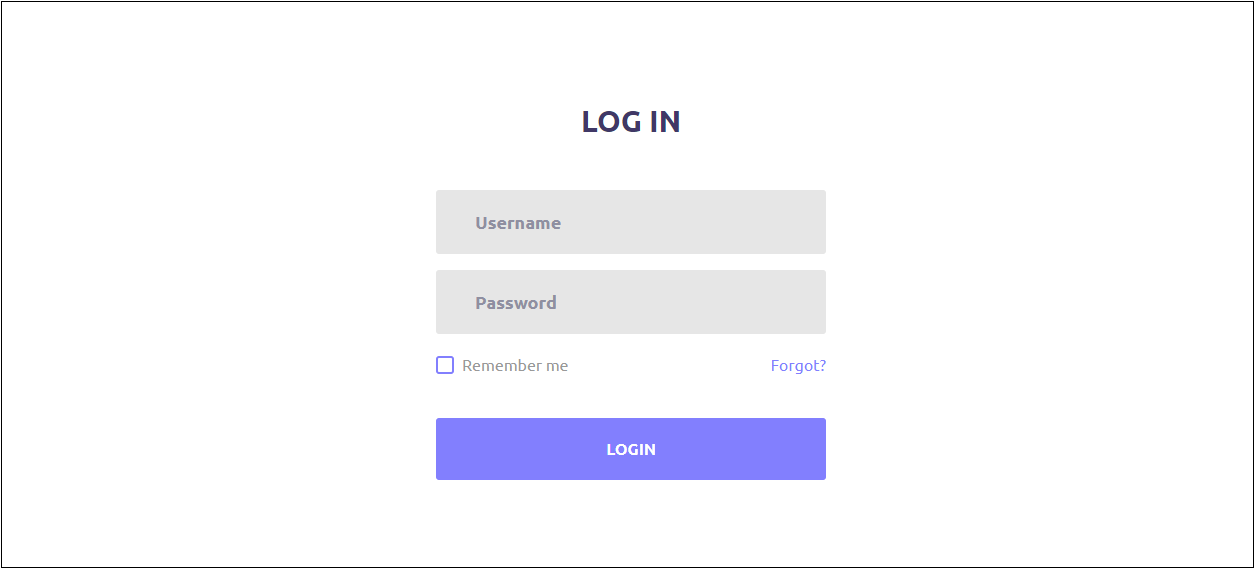
\includegraphics [width = 13cm, height= 6cm]{gambar/web/login}
		\caption{Halaman \textit{Log In}}
		\label{web-login}
		\end{figure}
		
		\vspace{-0.2cm}
		\begin{figure}[H]
		\center
		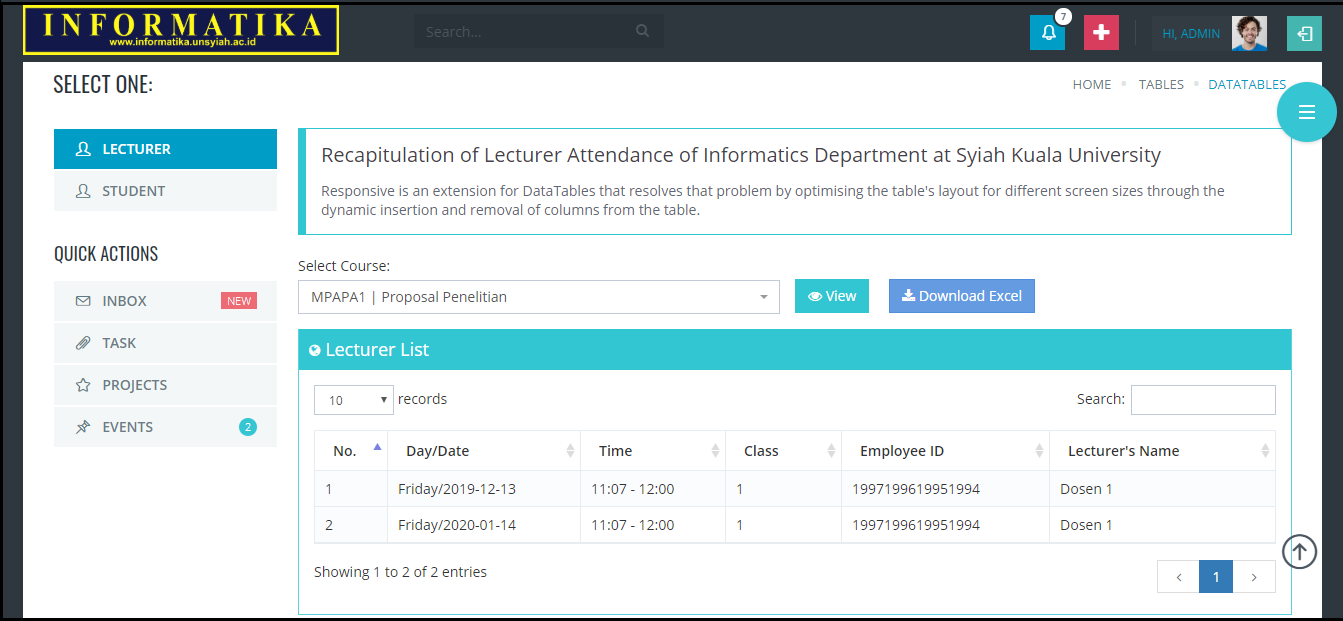
\includegraphics [width = 13cm, height= 6cm]{gambar/web/dashboard-dosen}
		\caption{Halaman Daftar Kehadiran Dosen}
		\label{web-daftar-dosen}
		\end{figure}
		
		\vspace{-0.2cm}
		\begin{figure}[H]
		\center
		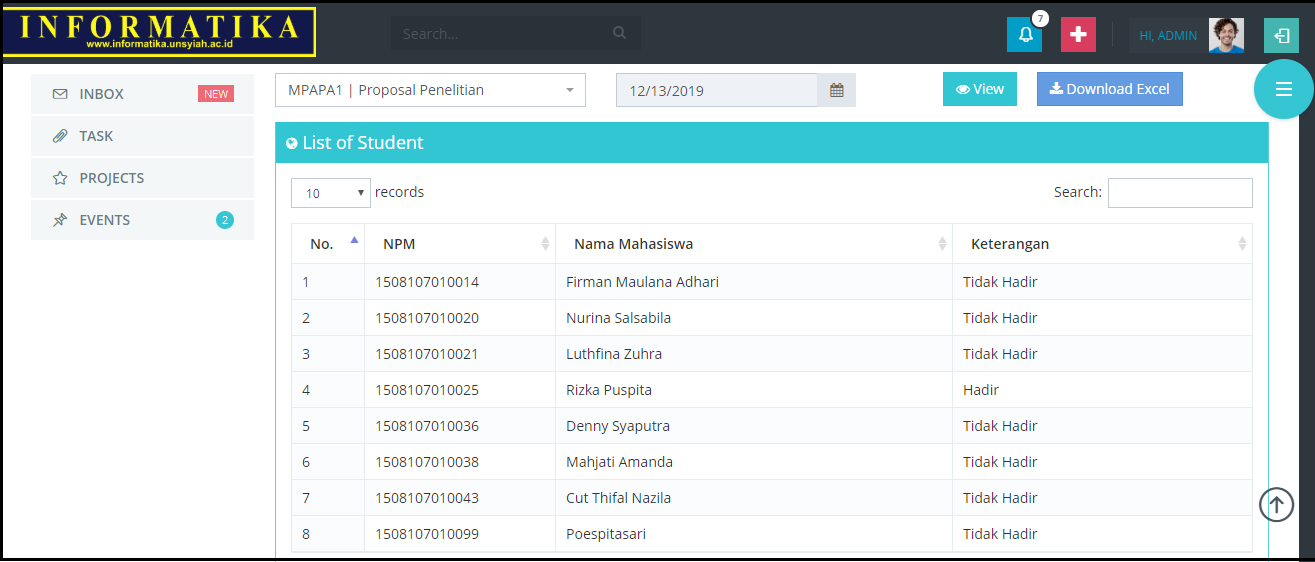
\includegraphics [width = 13cm, height= 6cm]{gambar/web/dashboard-mahasiswa}
		\caption{Halaman Daftar Kehadiran Mahasiswa}
		\label{web-daftar-mahasiswa}
		\end{figure}
		
		\vspace{-0.2cm}
		\begin{figure}[H]
		\center
		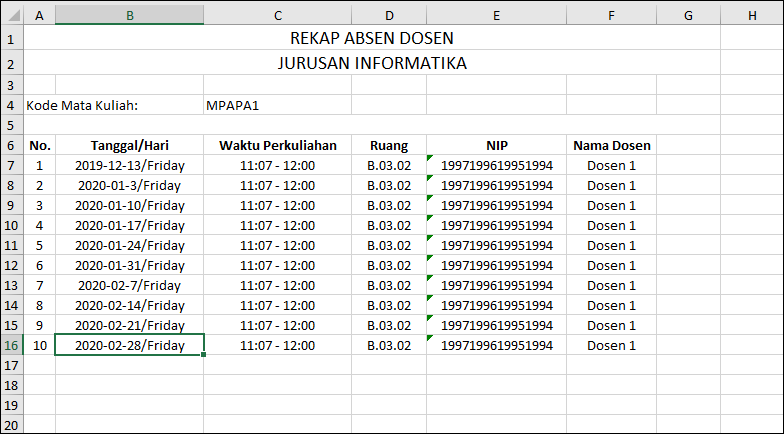
\includegraphics [width = 11cm, height= 6.3cm]{gambar/web/rekap-dosen}
		\caption{File Unduhan CSV Rekap Kehadiran Dosen}
		\label{web-csv-dosen}
		\end{figure}
		
		\vspace{-0.2cm}
		\begin{figure}[H]
		\center
		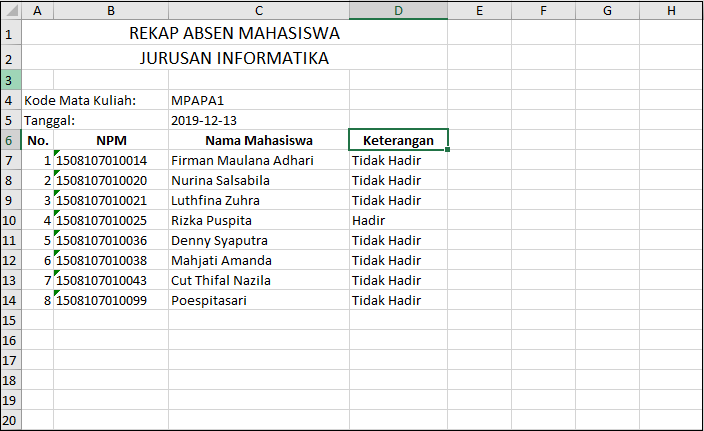
\includegraphics [width = 11cm, height= 6.3cm]{gambar/web/rekap-mahasiswa}
		\caption{File Unduhan CSV Rekap Kehadiran Mahasiswa}
		\label{web-csv-mahasiswa}
		\end{figure}
	
	\end{enumerate}
	
	\section{\uppercase{PENGUJIAN SISTEM}}
	\par Pengujian sistem dilakukan untuk melihat apakah sistem dapat berjalan dengan tepat sesuai dengan rancangan. Beberapa pengujian yang dilakukan pada penelitian ini adalah pengujian keakuratan klasifikasi menggunakan metode klasifikasi K-NN, pengujian usabilitas dengan metode SUS dan pengujian fungsionalitas menggunakan \textit{Blackbox}. 
		
\subsection{Pengujian Keakuratan Klasifikasi Menggunakan Metode Klasifikasi K-NN}
\begin{enumerate}

\item Pengujian Keakuratan Klasifikasi Reference Point

\par Pengujian ini dianalisis menggunakan metode klasifikasi K-NN. Pengujian ini bertujuan untuk menganalisis jenis penyebaran \textit{reference point} yang terbaik dengan membandingkan \textit{F-Measure} yang didapatkan dari setiap pengujian. Data \textit{training} yang digunakan pada penelitian ini sebanyak 764 data kekuatan sinyal dengan masing-masing 324 data kekuatan sinyal untuk \textit{reference point} acak, 440 data kekuatan sinyal untuk \textit{reference point} urut dan 160 sebagai data uji. Pengumpulan data \textit{training} dilakukan dengan cara melakukan pemetaan kekuataan sinyal yang telah dijelaskan pada \textbf{BAB III}. Hasil dari proses pengujian metode klasifikasi K-NN menunjukkan bahwa dengan K=5 untuk data kekuatan sinyal \textit{reference point} urut, memiliki rata-rata \textit{F-Measure} paling baik dengan nilai 78,60\% dibandingkan dengan parameter pengujian lainnya. Hasil pengujian menggunakan metode K-NN ini  dapat dilihat pada Tabel \ref{tabelfmeasure9}.
% Please add the following required packages to your document preamble:
% \usepackage{multirow}
\begin{table}[H]
\fontsize{9}{12}\selectfont
\center
\caption{Perbandingan F-Measure}
\label{tabelfmeasure9}
\begin{tabular}{|c|c|l|c|c|c|c|}
\hline
Jenis Titik           & Nilai K            & \multicolumn{1}{c|}{Kelas Label} & Precision & Recall  & F-Measure & Rata-Rata F-Measure      \\ \hline
\multirow{3}{*}{Urut} & \multirow{3}{*}{3} & B0302                            & 90,69\%   & 66,10\% & 76,47\%   & \multirow{3}{*}{78,52\%} \\ \cline{3-6}
                      &                    & E0207                            & 82,60\%   & 70,37\% & 76,00\%    &                          \\ \cline{3-6}
                      &                    & Luar Kelas                       & 83,09\%   & 83,09\% & 83,09\%   &                          \\ \hline
\multirow{3}{*}{Urut} & \multirow{3}{*}{5} & B0302                            & 90,69\%   & 66,10\% & 76,47\%   & \multirow{3}{*}{78,60\%} \\ \cline{3-6}
                      &                    & E0207                            & 81,25\%   & 72,22\% & 76,47\%   &                          \\ \cline{3-6}
                      &                    & Luar Kelas                       & 84,05\%   & 81,69\% & 82,85\%   &                          \\ \hline
\multirow{3}{*}{Urut} & \multirow{3}{*}{7} & B0302                            & 90,69\%   & 67,24\% & 72,20\%   & \multirow{3}{*}{77,42\%} \\ \cline{3-6}
                      &                    & E0207                            & 81,63\%   & 74,07\% & 76,60\%   &                          \\ \cline{3-6}
                      &                    & Luar Kelas                       & 85,29\%   & 81,69\% & 83,45\%   &                          \\ \hline
\multirow{3}{*}{Acak} & \multirow{3}{*}{3} & B0302                            & 97,36\%   & 60,65\% & 74,74\%   & \multirow{3}{*}{77,66\%} \\ \cline{3-6}
                      &                    & E0207                            & 78,00\%   & 73,58\% & 75,72\%   &                          \\ \cline{3-6}
                      &                    & Luar Kelas                       & 81,94\%   & 83,09\% & 82,51\%   &                          \\ \hline
\multirow{3}{*}{Acak} & \multirow{3}{*}{5} & B0302                            & 97,43\%   & 59,37\% & 73,78\%   & \multirow{3}{*}{76,07\%} \\ \cline{3-6}
                      &                    & E0207                            & 75,51\%   & 71,15\% & 73,26\%   &                          \\ \cline{3-6}
                      &                    & Luar Kelas                       & 80,55\%   & 81,69\% & 81,18\%   &                          \\ \hline
\multirow{3}{*}{Acak} & \multirow{3}{*}{7} & B0302                            & 97,36\%   & 59,67\% & 74,00\%    & \multirow{3}{*}{76,89\%} \\ \cline{3-6}
                      &                    & E0207                            & 76,47\%   & 73,58\% & 74,99\%   &                          \\ \cline{3-6}
                      &                    & Luar Kelas                       & 81,69\%   & 81,69\% & 81,69\%   &                          \\ \hline
\end{tabular}
\end{table}


\par Ilustrasi dari perbandingan F-Measure setiap parameter pengujian ditampilkan pada Gambar \ref{gambar-grafik-akurasi-klasifikasi-9-beacon}.
		\begin{figure}[H]
			\center
			\shadowbox
			{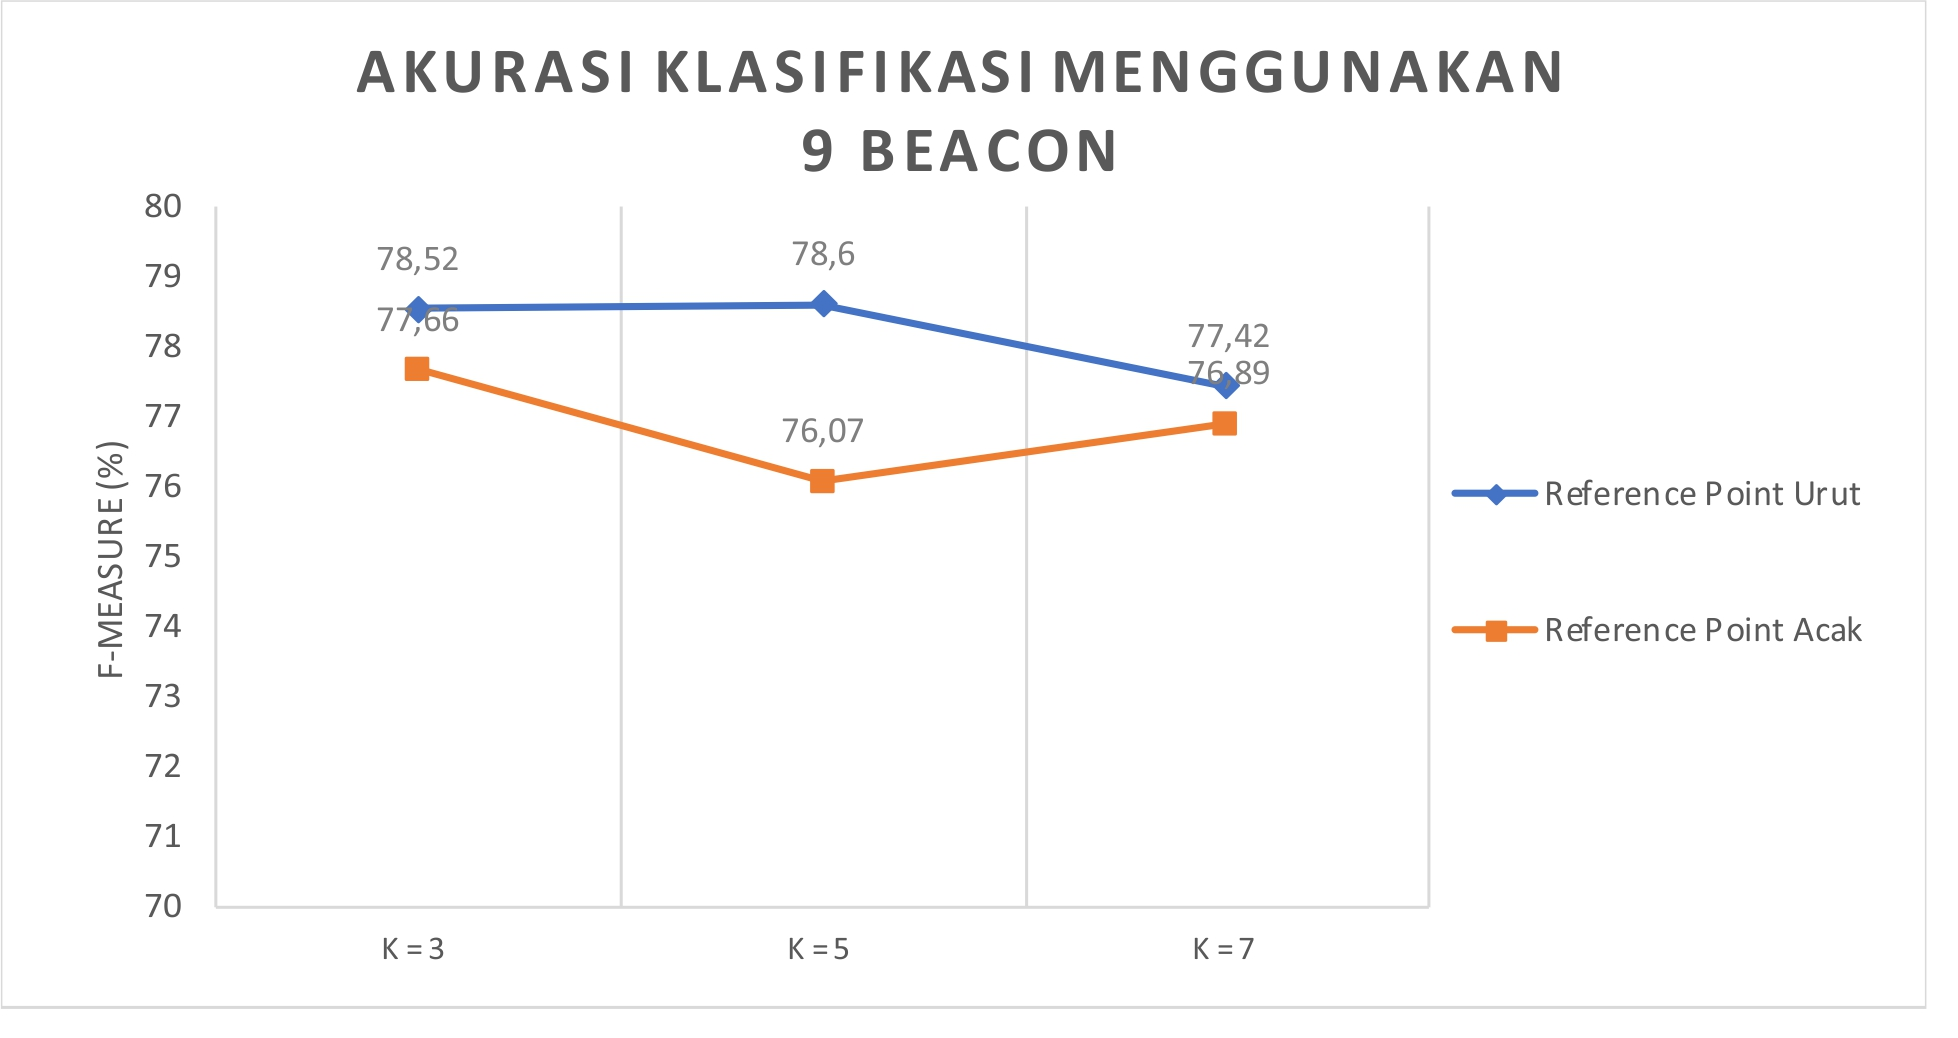
\includegraphics [width = 13cm, height= 7cm]{gambar/pengujian/grafik-akurasi-klasifikasi}}
			\caption{Grafik Perbandingan F-Measure dengan Menggunakan Parameter Pengujian yang Berbeda.}
			\label{gambar-grafik-akurasi-klasifikasi-9-beacon}
		\end{figure}
		
		\vspace{2cm}
		\par Pengambilan data uji dilakukan untuk menguji tingkat keberhasilan klasifikasi dengan melihat akurasi tertinggi bergantung pada parameter nilai K yang digunakan. Pada pengujian ini terdapat titik yang sering salah diprediksi yaitu sebanyak 6 dari 6 kali pengujian. Lokasi titik yang sering salah diprediksi ditandai dengan lingkaran bewarna biru yang ditampilkan dalam bentuk ilustrasi denah yang dapat dilihat pada Gambar \ref{gambar-denah-titik-uji-b0302} dan Gambar \ref{gambar-denah-titik-uji-e0207}.
\vspace{0.2cm}
		\begin{figure}[H]
			\center
			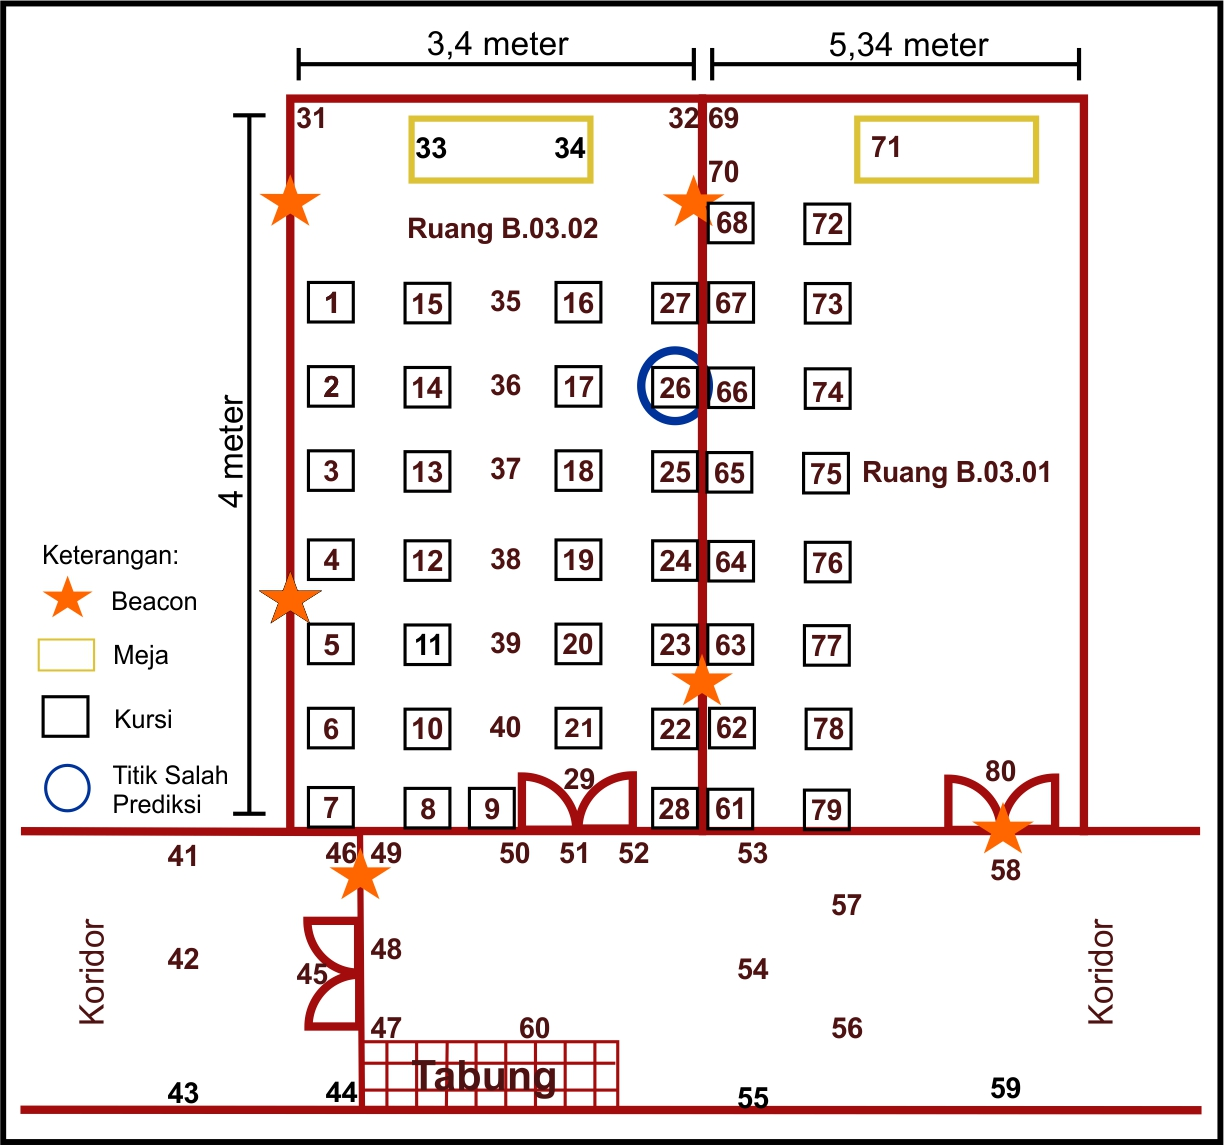
\includegraphics [width = 11cm, height= 9cm]{gambar/denah/B0302-Uji}
			\caption{Lokasi Titik yang Sering Salah Diprediksi di Kelas B.03.02.}
			\label{gambar-denah-titik-uji-b0302}
		\end{figure}
		
		\begin{figure}[H]
			\center
			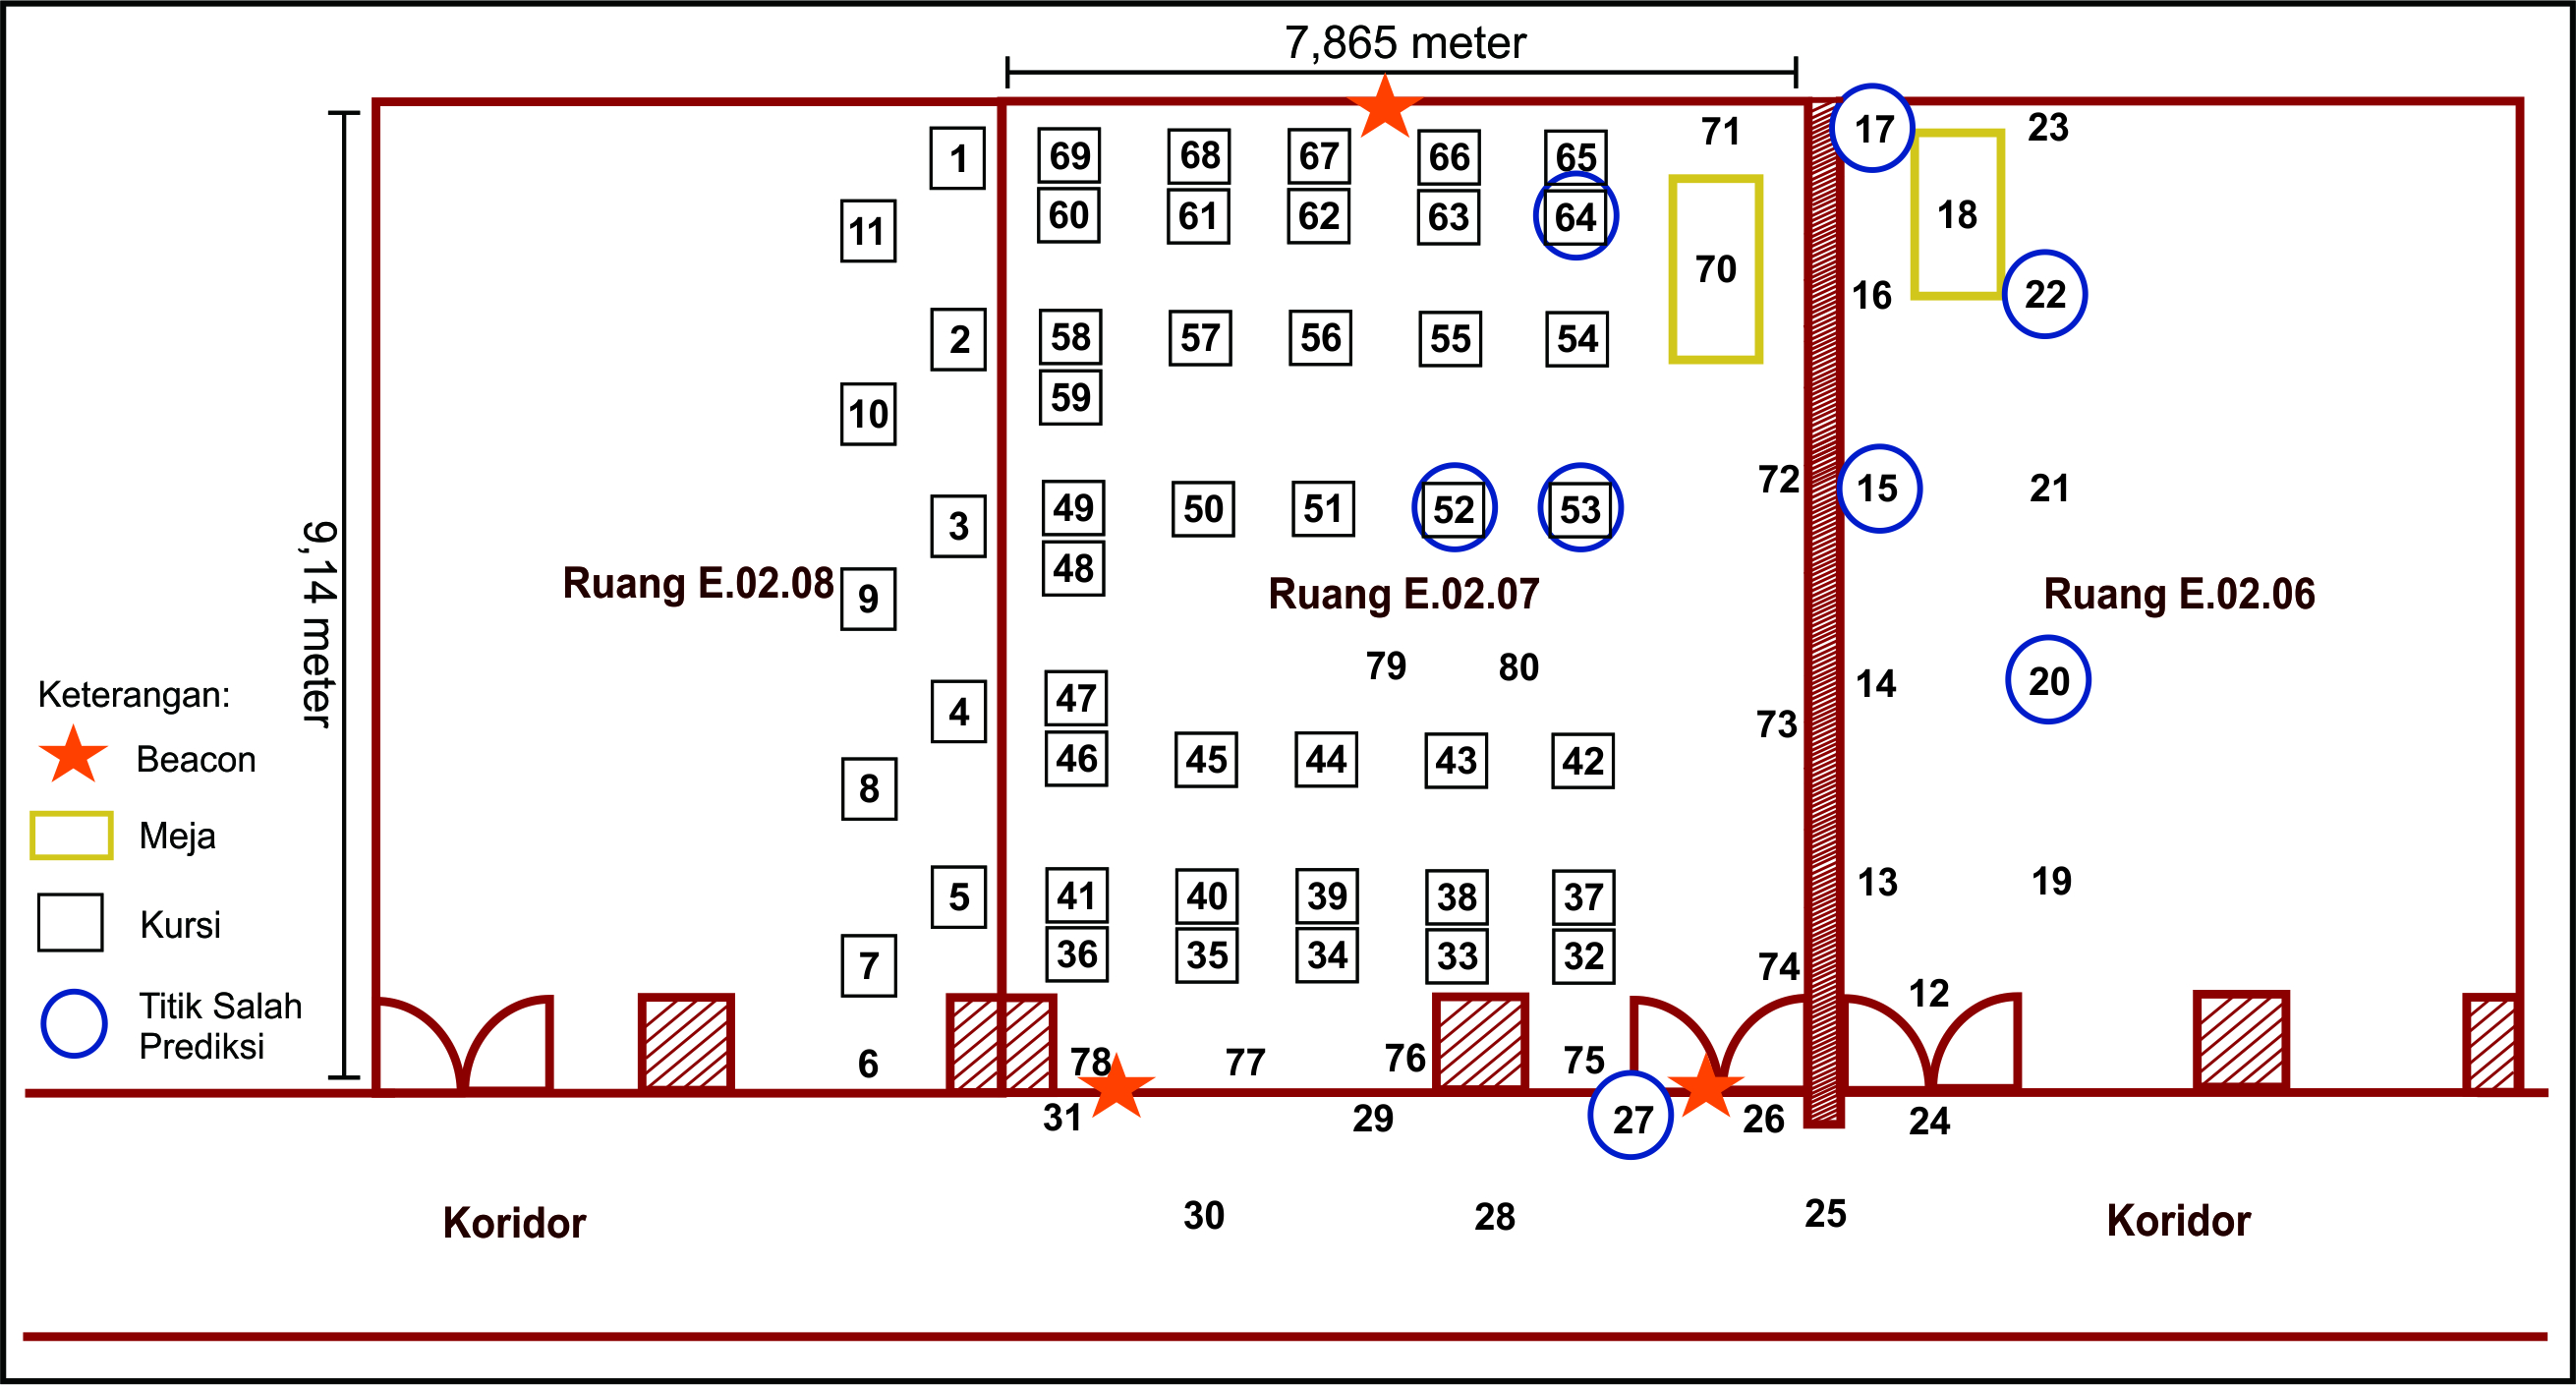
\includegraphics [width = 14cm, height= 8cm]{gambar/denah/E0207-Uji}
			\caption{Lokasi Titik yang Sering Salah Diprediksi di Kelas E.02.07.}
			\label{gambar-denah-titik-uji-e0207}
		\end{figure}
%batas batas batas batas batas batas batas batas batas batas batas batas batas

\item Pengujian Keakuratan Reference Point Berdasarkan Penggunaan Jumlah Beacon pada Ruang Kuliah B.03.02

\par Pengujian ini dianalisis menggunakan metode klasifikasi K-NN. Pengujian ini bertujuan untuk menganalisis tingkat keakuratan klasifikasi jenis \textit{reference point} terbaik yang digunakan dengan membandingkan penggunaan jumlah Beacon dengan melihat \textit{F-Measure} yang didapatkan dari setiap pengujian. Jumlah Beacon yang dibandingkan adalah 3 Beacon dan 6 Beacon. Data \textit{training} yang digunakan pada penelitian ini sebanyak 368 data kekuatan sinyal dengan masing-masing 120 data kekuatan sinyal untuk \textit{reference point} acak, 168 data kekuatan sinyal untuk \textit{reference point} urut dan 80 sebagai data uji. Pengumpulan data \textit{training} dilakukan dengan cara melakukan pemetaan kekuataan sinyal yang telah dijelaskan pada \textbf{BAB III}. Hasil dari proses pengujian metode klasifikasi K-NN menunjukkan bahwa dengan K=5 untuk data kekuatan sinyal \textit{reference point} acak menggunakan 6 Beacon, memiliki \textit{F-Measure} paling baik dengan nilai 96,20\% dibandingkan dengan parameter pengujian lainnya. Hasil pengujian menggunakan metode K-NN ini dapat dilihat secara detil pada Tabel \ref{tabelfmeasureee}.
% Please add the following required packages to your document preamble:
% \usepackage{multirow}
\begin{table}[H]
\fontsize{10}{12}\selectfont
\center
\caption{Perbandingan F-Measure}
\label{tabelfmeasureee}
\begin{tabular}{|c|c|l|c|c|c|}
\hline
Nilai K            & Jumlah BLE         & \multicolumn{1}{c|}{Jenis Titik} & Precision & Recall  & F-Measure \\ \hline
\multirow{2}{*}{3} & \multirow{2}{*}{3} & Urut                             & 67,24\%   & 97,50\% & 80,00\%    \\ \cline{3-6} 
                   &                    & Acak                             & 82,50\%   & 82,50\% & 82,50\%   \\ \hline
\multirow{2}{*}{5} & \multirow{2}{*}{3} & Urut                             & 67,24\%   & 97,50\% & 80,00\%    \\ \cline{3-6} 
                   &                    & Acak                             & 80,50\%   & 82,50\% & 81,50\%   \\ \hline
\multirow{2}{*}{7} & \multirow{2}{*}{3} & Urut                             & 67,24\%   & 97,50\% & 80,00\%    \\ \cline{3-6} 
                   &                    & Acak                             & 80,50\%   & 82,50\% & 81,50\%   \\ \hline
\multirow{2}{*}{3} & \multirow{2}{*}{6} & Urut                             & 90,70\%   & 97,50\% & 94,00\%    \\ \cline{3-6} 
                   &                    & Acak                             & 97,40\%   & 92,50\% & 95,00\%    \\ \hline
\multirow{2}{*}{5} & \multirow{2}{*}{6} & Urut                             & 90,70\%   & 97,50\% & 94,00\%    \\ \cline{3-6} 
                   &                    & Acak                             & 97,40\%   & 95,00\%  & 96,20\%   \\ \hline
\multirow{2}{*}{7} & \multirow{2}{*}{6} & Urut                             & 90,70\%   & 97,50\% & 94,00\%    \\ \cline{3-6} 
                   &                    & Acak                             & 97,40\%   & 92,50\% & 95,00\%    \\ \hline
\end{tabular}
\end{table}

\par Ilustrasi dari perbandingan F-Measure setiap parameter pengujian ditampilkan pada Gambar \ref{gambar-grafik-akurasi-klasifikasi-6-beacon}.
		\begin{figure}[H]
			\center
			\shadowbox
			{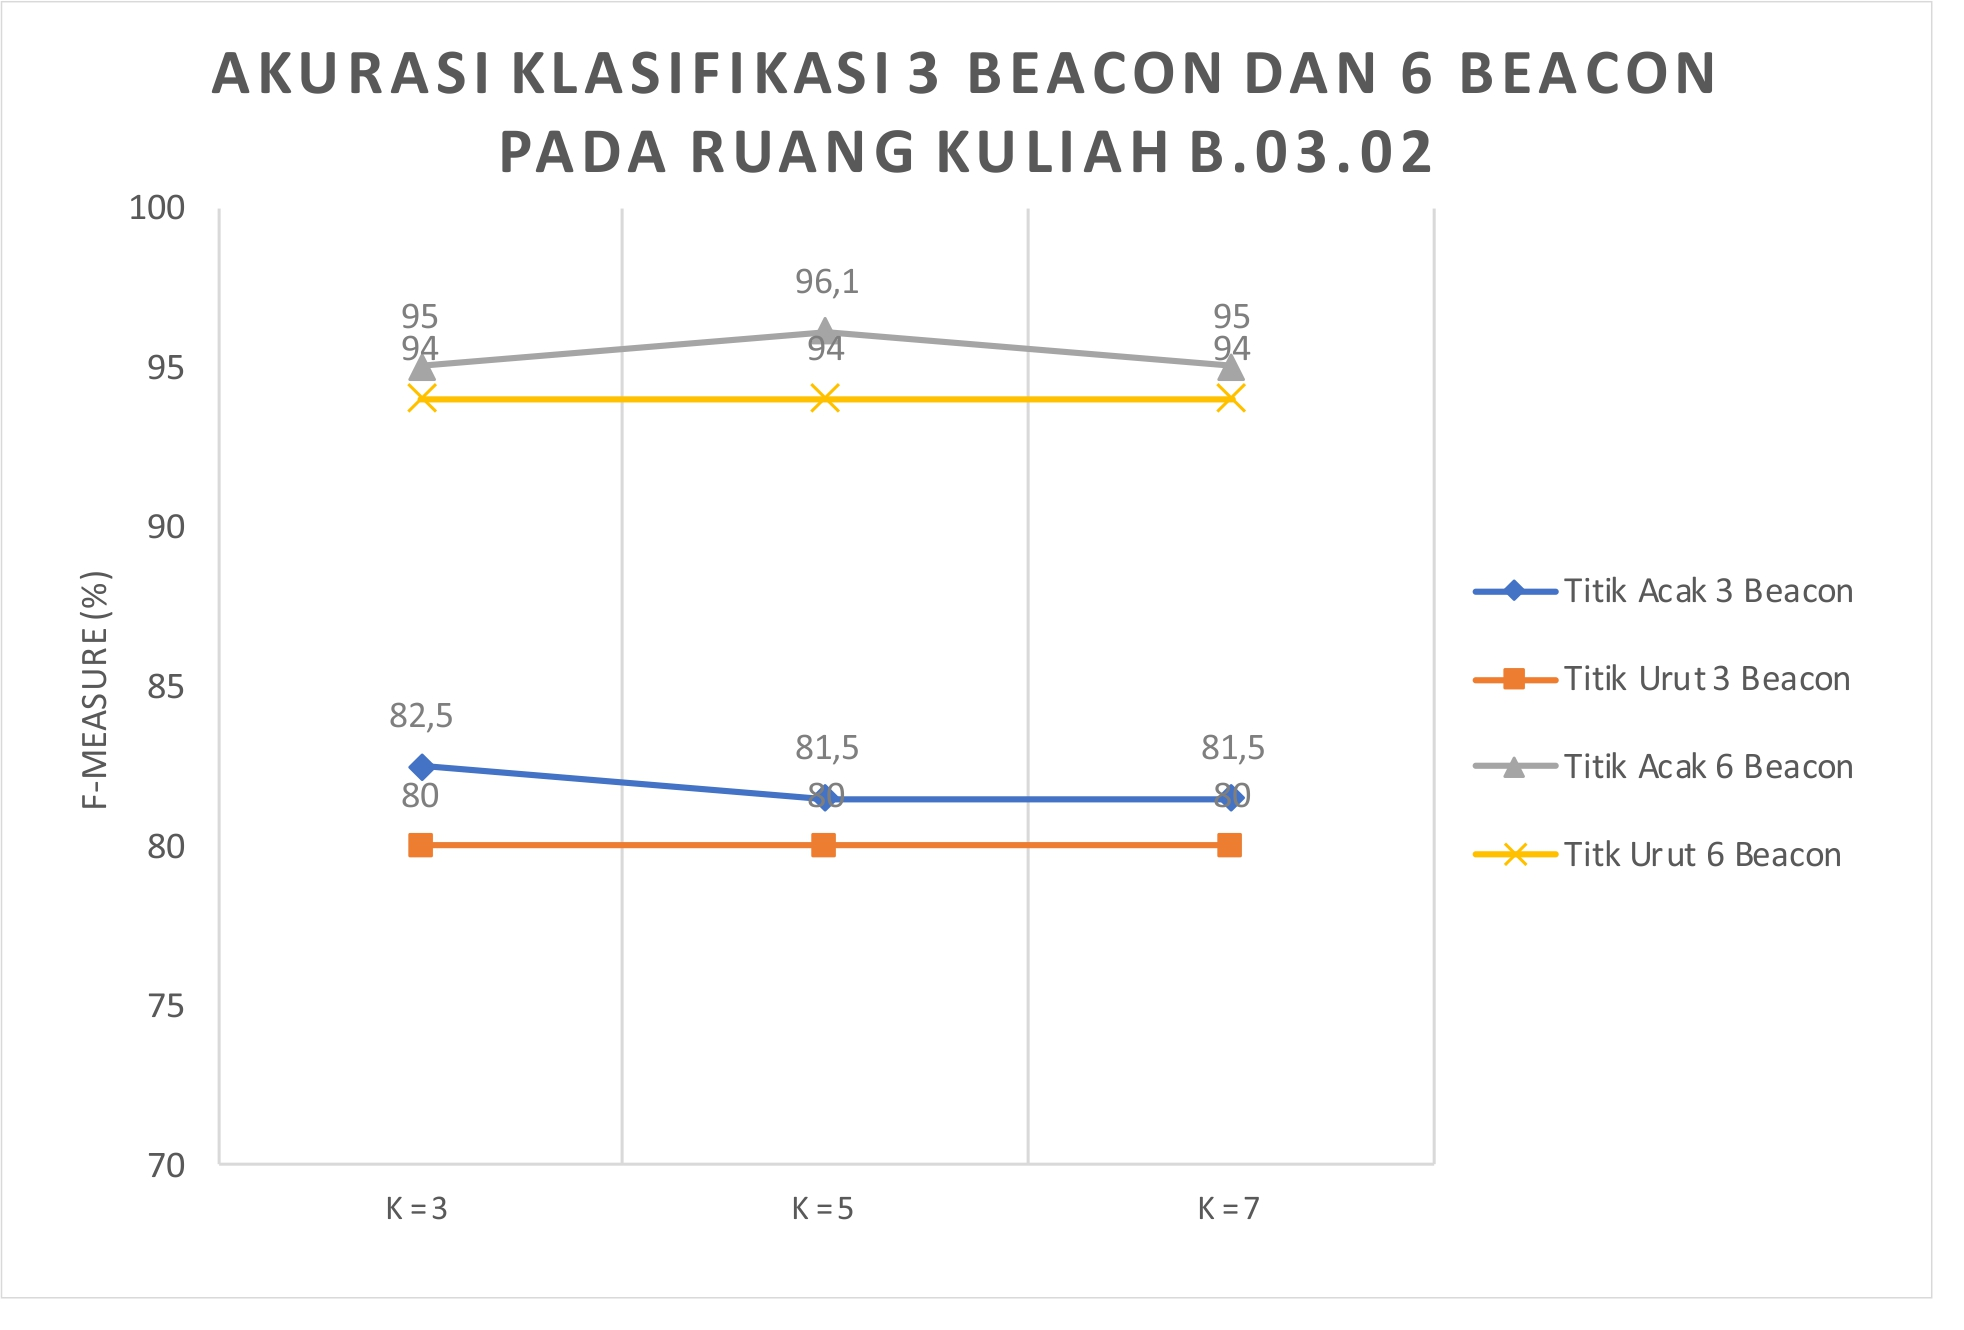
\includegraphics [width = 14cm, height= 8.7cm]{gambar/pengujian/grafik-akurasi-klasifikasi-kelas-b0302}}
			\caption{Grafik Perbandingan F-Measure dengan Menggunakan Parameter Pengujian yang Berbeda.}
			\label{gambar-grafik-akurasi-klasifikasi-6-beacon}
		\end{figure}
		
\par Berdasarkan hasil pengujian dengan parameter nilai K yang berbeda menggunakan 3 Beacon dan 6 Beacon berdasarkan jenis \textit{reference point} yang digunakan, menunjukkan bahwa penggunaan 6 Beacon mengurangi kesalahan prediksi titik dibandingkan dengan 3 Beacon. Ilustrasi perbandingan tersebut dapat ditampilkan pada Gambar \ref{gambar-grafik-titik-salah-prediksi}.	
		\begin{figure}[H]
			\center
			\shadowbox
			{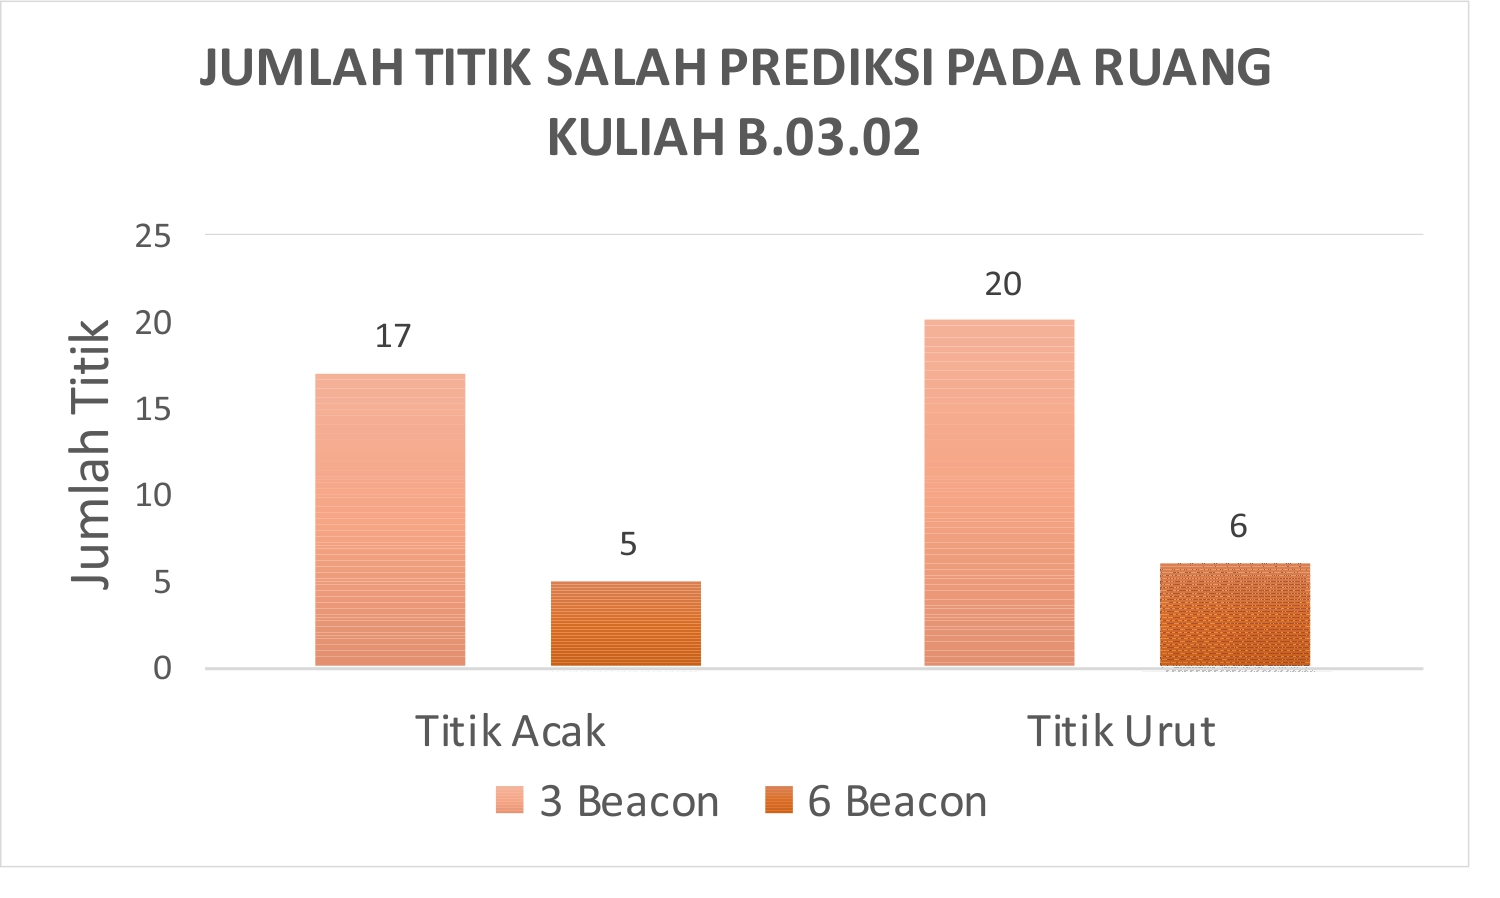
\includegraphics [width = 9cm, height= 5cm]{gambar/pengujian/grafik-titik-salah-prediksi}}
			\caption{Grafik Jumlah Titik yang Salah Diprediksi.}
			\label{gambar-grafik-titik-salah-prediksi}
		\end{figure}
		

%batas batas batas batas batas batas batas batas batas batas batas batas batas	
\end{enumerate} 

\subsection{Pengujian Usabilitas Menggunakan Metode SUS}
\par Pengujian usabilitas bertujuan untuk menguji kelayakan dan kegunaan dari sistem yang akan digunakan oleh pengguna. Sebelum melakukan pengujian ini, adapun \textit{Test Plan} yang telah dibuat untuk yang dapat dilihat pada Tabel \ref{testplan-aplikasi-dosen} dan Tabel \ref{testplan-aplikasi-mahasiswa}.

\begin{table}[H]
\fontsize{10}{12}\selectfont
\center
\caption{\textit{Test Plan} Aplikasi Kehadiran Dosen}
\label{testplan-aplikasi-dosen}
\begin{tabular}{|l|l|l|l|l|}
\hline
\multicolumn{5}{|c|}{\textbf{Test Plan Aplikasi Kehadiran Dosen}}                                                                                                                                                                                                          \\ \hline
\multicolumn{5}{|l|}{\begin{tabular}[c]{@{}l@{}}Lokasi:\\ Ruang kuliah B.03.02 \\Ruang Kuliah E.03.07\end{tabular}}                                                                                                                                                                               \\ \hline
\multicolumn{5}{|l|}{\begin{tabular}[c]{@{}l@{}}Skenario:\\ 1. Dosen melakukan \textit{log in} ke aplikasi.\\ 2. Dosen memahami tampilan halaman beranda. \\ 3. Dosen melihat daftar mahasiswa yang mengambil suatu mata kuliah. \\ 4. Dosen memulai proses kehadiran.\\ 5. Dosen melihat hasil prediksi lokasi yang dilakukan oleh aplikasi.\end{tabular}} \\ \hline
\multicolumn{5}{|l|}{\begin{tabular}[c]{@{}l@{}}Alat:\\ 1. Smartphone Android\\ 2. Beacon\end{tabular}}                                                                                                                                                                    \\ \hline
\multicolumn{5}{|l|}{\begin{tabular}[c]{@{}l@{}}Hasil:\\ Hasil pengujian dapat dilihat pada tabel dan lampiran.\end{tabular}}                                                                                                                                              \\ \hline
\end{tabular}
\end{table}

\begin{table}[H]
\fontsize{10}{12}\selectfont
\center
\caption{\textit{Test Plan} Aplikasi Kehadiran Mahasiswa}
\label{testplan-aplikasi-mahasiswa}
\begin{tabular}{|l|l|l|l|l|}
\hline
\multicolumn{5}{|c|}{\textbf{Test Plan Aplikasi Kehadiran Mahasiswa}}                                                                                                                                                                                                                                                                             \\ \hline
\multicolumn{5}{|l|}{\begin{tabular}[c]{@{}l@{}}Lokasi:\\ Ruang kuliah B.03.02 \\Ruang Kuliah E.03.07\end{tabular}}                                                                                                                                                                                                                                                      \\ \hline
\multicolumn{5}{|l|}{\begin{tabular}[c]{@{}l@{}}Skenario:\\ 1. Mahasiswa melakukan \textit{log in} ke aplikasi.\\ 2. Mahasiswa melihat halaman profil data diri.\\ 3. Mahasiswa melihat daftar mata kuliah yang diambil.\\ 4. Mahasiswa memulai proses kehadiran.\\ 5. Mahasiswa melihat hasil prediksi lokasi yang dilakukan oleh aplikasi.\end{tabular}} \\ \hline
\multicolumn{5}{|l|}{\begin{tabular}[c]{@{}l@{}}Alat:\\ 1. Smartphone Android\\ 2. Beacon\end{tabular}}                                                                                                                                                                                                                                           \\ \hline
\multicolumn{5}{|l|}{\begin{tabular}[c]{@{}l@{}}Hasil:\\ Hasil pengujian dapat dilihat pada tabel dan lampiran.\end{tabular}}                                                                                                                                                                                                                     \\ \hline
\end{tabular}
\end{table}

\par Pengujian dengan metode SUS dilakukan dengan memberikan kuisioner kepada responden. Kuisioner tersebut berisi 10 pertanyaan seperti yang telah dibahas pada. Pengujian Aplikasi Kehadiran Dosen memiliki responden berjumlah 5 orang sedangkan pengujian Aplikasi Kehadiran Mahasiswa memiliki responden berjumlah 9 orang. Hasil skor pengujian metode SUS yang dilakukan dapat dilihat pada Tabel \ref{sus-aplikasi-dosen} dan Tabel \ref{sus-aplikasi-mahasiswa} berikut. 
%TABEL SUS APLIKASI DOSEN%
\begin{table}[H]
\fontsize{10}{12}\selectfont
\center
\caption{Hasil Pengujian SUS Aplikasi Kehadiran Dosen}
\label{sus-aplikasi-dosen}
\begin{tabular}{|c|c|c|c|c|c|c|c|c|c|c|c|}
\hline
\multirow{2}{*}{\textbf{Responden}} & \multicolumn{10}{c|}{\textbf{Kode Pertanyaan}}                                                                                                                  & \multirow{2}{*}{\textbf{Skor SUS}} \\ \cline{2-11}
                                    & \textbf{R1} & \textbf{R2} & \textbf{R3} & \textbf{R4} & \textbf{R5} & \textbf{R6} & \textbf{R7} & \textbf{R8} & \textbf{R9} & \multicolumn{1}{l|}{\textbf{R10}} &                                    \\ \hline
1                                   & 3           & 2           & 4           & 1           & 4           & 4           & 4           & 3           & 4           & 2                                 & 67,5                               \\ \hline
2                                   & 5           & 2           & 5           & 4           & 4           & 2           & 4           & 2           & 4           & 5                                 & 67,5                               \\ \hline
3                                   & 4           & 2           & 4           & 1           & 4           & 2           & 4           & 1           & 4           & 4                                 & 75,0                                 \\ \hline
4                                   & 5           & 1           & 5           & 2           & 5           & 2           & 5           & 1           & 5           & 1                                 & 95,0                                 \\ \hline
5                                   & 5           & 2           & 5           & 1           & 4           & 2           & 5           & 2           & 5           & 2                                 & 87,5                               \\ \hline
\multicolumn{11}{|c|}{\textbf{Rata - Rata}}                                                                                                                                                           & \textbf{78,5}                      \\ \hline
\end{tabular}
\end{table}

%TABEL SUS APLIKASI MAHASISWA%
\begin{table}[H]
\fontsize{10}{12}\selectfont
\center
\caption{Hasil Pengujian SUS Aplikasi Kehadiran Mahasiswa}
\label{sus-aplikasi-mahasiswa}
\begin{tabular}{|c|c|c|c|c|c|c|c|c|c|c|c|}
\hline
\multirow{2}{*}{\textbf{Responden}} & \multicolumn{10}{c|}{\textbf{Kode Pertanyaan}}                                                                                                                  & \multirow{2}{*}{\textbf{Skor SUS}} \\ \cline{2-11}
                                    & \textbf{R1} & \textbf{R2} & \textbf{R3} & \textbf{R4} & \textbf{R5} & \textbf{R6} & \textbf{R7} & \textbf{R8} & \textbf{R9} & \multicolumn{1}{l|}{\textbf{R10}} &                                    \\ \hline
1                                   & 5           & 1           & 4           & 1           & 4           & 1           & 5           & 1           & 5           & 1                                 & 95,0                                 \\ \hline
2                                   & 5           & 2           & 4           & 2           & 4           & 2           & 4           & 2           & 2           & 2                                 & 72,5                               \\ \hline
3                                   & 5           & 2           & 5           & 2           & 5           & 1           & 5           & 1           & 5           & 2                                 & 92,5                               \\ \hline
4                                   & 5           & 1           & 5           & 1           & 5           & 1           & 5           & 1           & 5           & 1                                 & 100,0                                \\ \hline
5                                   & 5           & 1           & 5           & 2           & 5           & 1           & 5           & 1           & 5           & 2                                 & 95,0                                 \\ \hline
6                                   & 5           & 2           & 4           & 1           & 4           & 2           & 4           & 1           & 5           & 2                                 & 85,0                                 \\ \hline
7                                   & 5           & 3           & 4           & 2           & 4           & 2           & 4           & 2           & 3           & 5                                 & 65,0                                 \\ \hline
8                                   & 4           & 1           & 5           & 2           & 4           & 2           & 4           & 1           & 5           & 4                                 & 80,0                                 \\ \hline
9                                   & 5           & 1           & 5           & 2           & 5           & 2           & 5           & 2           & 5           & 2                                 & 90,0                                 \\ \hline
\multicolumn{11}{|c|}{\textbf{Rata - Rata}}                                                                                                                                                             & \textbf{86,1}                      \\ \hline
\end{tabular}
\end{table}

\par Berdasarkan hasil pengujian SUS yang telah dilakukan diatas, hasil rata-rata pengujian Aplikasi Kehadiran Dosen mendapatkan skor sebesar 78,5\% sedangkan hasil rata-rata pengujian Aplikasi Kehadiran Mahasiswa mendapatkan skor sebesar 86,1\%. Dapat dilihat bahwa kedua aplikasi yang telah dibangun memiliki skor interpretasi \textbf{"dapat diterima"} berdasarkan Tabel 3.4.  

\subsection{Pengujian Fungsionalitas Menggunakan Blackbox}
\par Pengujian \textit{Blackbox} dilakukan dengan tujuan untuk menguji fungsionalitas dari aplikasi dengan menjalankan aplikasi tersebut apakah sesuai dengan alur bisnis yang diinginkan. Pengujian ini melihat fungsi yang tidak sesuai pada aplikasi dan kesalahan-kesalahan aplikasi dalam mengerjakan suatu perintah. Pengujian ini dilakukan pada Aplikasi Mapping, Aplikasi Kehadiran Dosen, Aplikasi Kehadiran Mahasiswa, dan Aplikasi Web Rekap Kehadiran Dosen dan Mahasiswa. Beberapa fitur aplikasi yang diuji menggunakan \textit{Blackbox Testing} dapat dilihat pada Tabel \ref{blackbox-aplikasi-mapping}, Tabel \ref{blackbox-aplikasi-dosen}, Tabel \ref{blackbox-aplikasi-mahasiswa}, dan Tabel \ref{blackbox-web-admin}.
%TABEL APLIKASI MAPPING%
\begin{table}[H]
\fontsize{10}{12}\selectfont
\center
\caption{Pengujian \textit{Blackbox} Aplikasi Mapping}
\label{blackbox-aplikasi-mapping}
\begin{tabular}{|c|l|l|l|c|}
\hline
\textbf{No.} & \multicolumn{1}{c|}{\textbf{Nama Pengujian}}                                       & \multicolumn{1}{c|}{\textbf{Skenario}}                                                                                        & \multicolumn{1}{c|}{\textbf{Tampilan}}                                                                    & \textbf{Hasil}                \\ \hline
1.           & \begin{tabular}[c]{@{}l@{}}Menghidupkan \\ Bluetooth\end{tabular}                  & \begin{tabular}[c]{@{}l@{}}Klik tombol \textbf{Allow} \\ pada notifikasi yang\\ muncul\end{tabular}                                  & \begin{tabular}[c]{@{}l@{}}Bluetooth akan \\ hidup\end{tabular}                                           & Berhasil                      \\ \hline
2.           & \begin{tabular}[c]{@{}l@{}}Lakukan proses \\ pemindaian \\ sinyal BLE\end{tabular} & Klik tombol \textbf{"Scan"}                                                                                                            & \begin{tabular}[c]{@{}l@{}}Muncul nama BLE, \\ MAC Address BLE \\ dan kekuatan sinyal \\ BLE\end{tabular} & Berhasil                      \\ \hline
3.           & \begin{tabular}[c]{@{}l@{}}Menyimpan data \\ ke tabel titik acak\end{tabular}      & \begin{tabular}[c]{@{}l@{}}Mengisi nama ruang \\ kemudian klik tombol \\ \textbf{Save to} dan pilih \\ tabel titik acak\end{tabular} & \begin{tabular}[c]{@{}l@{}}Muncul \textit{pop up} \\ untuk memilih \\ tabel\end{tabular}                           & Berhasil                      \\ \hline
4.           & \begin{tabular}[c]{@{}l@{}}Menyimpan data \\ ke tabel titik urut\end{tabular}      & \begin{tabular}[c]{@{}l@{}}Mengisi nama ruang \\ kemudian klik tombol \\ \textbf{Save to} dan pilih \\ tabel titik urut\end{tabular} & \begin{tabular}[c]{@{}l@{}}Muncul \textit{pop up} \\ untuk memilih \\ tabel\end{tabular}                           & Berhasil                      \\ \hline
5.           & \begin{tabular}[c]{@{}l@{}}Melihat data \\ yang tersimpan\end{tabular}             & \begin{tabular}[c]{@{}l@{}}Klik tombol \\ \textbf{Show Data}\end{tabular}                                                            & \begin{tabular}[c]{@{}l@{}}Diarahkan ke \\ halaman daftar \\ data yang tersimpan\end{tabular}             & Berhasil                      \\ \hline
6.           & \begin{tabular}[c]{@{}l@{}}Menghapus data \\ yang tersimpan\end{tabular}           & \begin{tabular}[c]{@{}l@{}}Klik icon \textbf{Tong} \\ \textbf{Sampah}\end{tabular}                                                              & \begin{tabular}[c]{@{}l@{}}Muncul notifikasi \\ dan konfirmasi \\ untuk menghapus \\ data\end{tabular}    & \multicolumn{1}{l|}{Berhasil} \\ \hline
\end{tabular}
\end{table}

%BLACKBOX APLIKASI DOSEN%
\begin{table}[H]
\fontsize{10}{12}\selectfont
\center
\caption{Pengujian \textit{Blackbox } Aplikasi Kehadiran Dosen}
\label{blackbox-aplikasi-dosen}
\begin{tabular}{|c|l|l|l|c|}
\hline
No. & \multicolumn{1}{c|}{\textbf{Nama Pengujian}}                                                                              & \multicolumn{1}{c|}{\textbf{Skenario}}                                                                                    & \multicolumn{1}{c|}{\textbf{Tampilan}}                                                                                  & Hasil    \\ \hline
1.  & \begin{tabular}[c]{@{}l@{}}Melakukan \textit{log in} \\ ke aplikasi\end{tabular}                                          & \begin{tabular}[c]{@{}l@{}}Klik tombol \textbf{Submit} \\ setelah selesai \\ mengisi form \textit{log in}\end{tabular}             & \begin{tabular}[c]{@{}l@{}}Diarahkan ke \\ halaman beranda \\ aplikasi apabila \\ berhasil \textit{log in}\end{tabular} & Berhasil \\ \hline
2.  & \begin{tabular}[c]{@{}l@{}}Melihat informasi \\ suatu mata kuliah\end{tabular}                                   & \begin{tabular}[c]{@{}l@{}}Klik salah satu daftar \\ mata kuliah\end{tabular}                                    & \begin{tabular}[c]{@{}l@{}}Diarahkan ke \\ halaman informasi \\ mata kuliah\end{tabular}                       & Berhasil \\ \hline
3.  & \begin{tabular}[c]{@{}l@{}}Menghidupkan \\ Bluetooth\end{tabular}                                                & \begin{tabular}[c]{@{}l@{}}Klik tombol \textbf{Allow} \\ pada notifikasi yang \\ muncul\end{tabular}                      & \begin{tabular}[c]{@{}l@{}}Bluetooth akan \\ menyala\end{tabular}                                              & Berhasil \\ \hline
4.  & \begin{tabular}[c]{@{}l@{}}Melihat daftar \\ nama mahasiswa \\ yang mengambil  \\ suatu mata kuliah\end{tabular} & \begin{tabular}[c]{@{}l@{}}Klik tombol \\ \textbf{Show Students} pada \\ halaman informasi \\ mata kuliah\end{tabular}    & \begin{tabular}[c]{@{}l@{}}Diarahkan ke \\ halaman daftar \\ nama mahasiswa\end{tabular}                       & Berhasil \\ \hline
5.  & \begin{tabular}[c]{@{}l@{}}Memulai proses \\ kehadiran\end{tabular}                                              & \begin{tabular}[c]{@{}l@{}}Klik tombol \\ \textbf{Start Attendance} \\ pada halaman \\ informasi mata kuliah\end{tabular} & \begin{tabular}[c]{@{}l@{}}Secara \textit{background} \\ \textit{proccess} aplikasi \\ akan memproses \\ kehadiran\end{tabular}  & Berhasil \\ \hline
\end{tabular}
\end{table}

%BLACKBOX APLIKASI MAHASISWA%
\begin{table}[H]
\fontsize{10}{12}\selectfont
\center
\caption{Pengujian \textit{Blackbox} Aplikasi Kehadiran Mahasiswa}
\label{blackbox-aplikasi-mahasiswa}
\begin{tabular}{|c|l|l|l|c|}
\hline
No. & \multicolumn{1}{c|}{\textbf{Nama Pengujian}}                                                   & \multicolumn{1}{c|}{\textbf{Skenario}}                                                                                    & \multicolumn{1}{c|}{\textbf{Tampilan}}                                                                                  & Hasil                         \\ \hline
1.  & \begin{tabular}[c]{@{}l@{}}Melakukan \textit{log in}\\ ke aplikasi\end{tabular}                & \begin{tabular}[c]{@{}l@{}}Klik tombol \textbf{Submit} \\ setelah selesai \\ mengisi form \textit{log in}\end{tabular}             & \begin{tabular}[c]{@{}l@{}}Diarahkan ke \\ halaman beranda \\ aplikasi apabila \\ berhasil \textit{log in}\end{tabular} & Berhasil                      \\ \hline
2.  & \begin{tabular}[c]{@{}l@{}}Melihat daftar \\ mata kuliah \\ yang diambil\end{tabular} & Klik icon \textbf{My Course}                                                                                              & \begin{tabular}[c]{@{}l@{}}Diarahkan ke \\ halaman daftar \\ mata kuliah\end{tabular}                          & Berhasil                      \\ \hline
3.  & \begin{tabular}[c]{@{}l@{}}Melihat profil \\ data diri\end{tabular}                   & Klik icon \textbf{My Profile                                                                                            } & \begin{tabular}[c]{@{}l@{}}Diarahkan ke \\ halaman profil\end{tabular}                                         & \multicolumn{1}{l|}{Berhasil} \\ \hline
4.  & \begin{tabular}[c]{@{}l@{}}Menghidupkan \\ Bluetooth\end{tabular}                     & \begin{tabular}[c]{@{}l@{}}Klik tombol \textbf{Allow} \\ pada notifikasi \\ yang muncul\end{tabular}                      & \begin{tabular}[c]{@{}l@{}}Bluetooth akan \\ menyala\end{tabular}                                              & Berhasil                      \\ \hline
5.  & \begin{tabular}[c]{@{}l@{}}Memulai \\ proses kehadiran\end{tabular}                   & \begin{tabular}[c]{@{}l@{}}Klik tombol \\ \textbf{Start Attendance} \\ pada salah satu \\ daftar mata kuliah\end{tabular} & \begin{tabular}[c]{@{}l@{}}Secara \textit{background} \\ \textit{proccess} aplikasi \\ akan memproses \\ kehadiran\end{tabular}  & Berhasil                      \\ \hline
\end{tabular}
\end{table}

%BLACKBOX WEB ADMIN%
\begin{table}[H]
\fontsize{10}{12}\selectfont
\center
\caption{Pengujian \textit{Blackbox} Aplikasi Web Rekap Kehadiran Dosen dan Mahasiswa}
\label{blackbox-web-admin}
\begin{tabular}{|c|l|l|l|c|}
\hline
No. & \multicolumn{1}{c|}{\textbf{Nama Pengujian}}                                                   & \multicolumn{1}{c|}{\textbf{Skenario}}                                                                                    & \multicolumn{1}{c|}{\textbf{Tampilan}}                                                                                  & Hasil                         \\ \hline
1.  & \begin{tabular}[c]{@{}l@{}}Melakukan \textit{log in}\\ ke aplikasi\end{tabular}                & \begin{tabular}[c]{@{}l@{}}Klik tombol \\ \textbf{Submit} setelah \\ selesai mengisi \\ form \textit{log in}\end{tabular}          & \begin{tabular}[c]{@{}l@{}}Diarahkan ke \\ halaman beranda \\ aplikasi apabila \\ berhasil \textit{log in}\end{tabular} & Berhasil                      \\ \hline
2.  & \begin{tabular}[c]{@{}l@{}}Melihat daftar \\ mata kuliah \\ yang diambil\end{tabular} & \begin{tabular}[c]{@{}l@{}}Klik icon \\ \textbf{My Course}\end{tabular}                                                   & \begin{tabular}[c]{@{}l@{}}Diarahkan ke \\ halaman daftar \\ mata kuliah\end{tabular}                          & Berhasil                      \\ \hline
3.  & \begin{tabular}[c]{@{}l@{}}Melihat profil \\ data diri\end{tabular}                   & \begin{tabular}[c]{@{}l@{}}Klik icon \\ \textbf{My Profile}\end{tabular}                                                  & \begin{tabular}[c]{@{}l@{}}Diarahkan ke \\ halaman profil\end{tabular}                                         & \multicolumn{1}{l|}{Berhasil} \\ \hline
4.  & \begin{tabular}[c]{@{}l@{}}Menghidupkan \\ Bluetooth\end{tabular}                     & \begin{tabular}[c]{@{}l@{}}Klik tombol \\ \textbf{Allow} pada \\ notifikasi yang\\ muncul\end{tabular}                    & \begin{tabular}[c]{@{}l@{}}Bluetooth akan \\ menyala\end{tabular}                                              & Berhasil                      \\ \hline
5.  & \begin{tabular}[c]{@{}l@{}}Memulai \\ proses kehadiran\end{tabular}                   & \begin{tabular}[c]{@{}l@{}}Klik tombol \\ \textbf{Start Attendance} \\ pada salah satu \\ daftar mata kuliah\end{tabular} & \begin{tabular}[c]{@{}l@{}}Secara \textit{background} \\ \textit{proccess} aplikasi \\ akan memproses \\ kehadiran\end{tabular}  & Berhasil                      \\ \hline
\end{tabular}
\end{table}

%AKHIR DARI TABEL%
\par Berdasarkan hasil \textit{Blackbox Testing} dari tabel diatas menunjukkan bahwa Aplikasi Mapping, Aplikasi Kehadiran Dosen, Aplikasi Kehadiran Mahasiswa, dan Aplikasi Web Rekap Kehadiran Dosen dan Mahasiswa dapat berjalan dengan baik dibuktikan dengan  \textbf{"berhasil"} pada kolom hasil pengujian masing-masing fitur yang dikerjakan.


\begin{comment}
\bibliography{daftar-pustaka}
\end{comment}